\documentclass[twoside]{book}

% Packages required by doxygen
\usepackage{fixltx2e}
\usepackage{calc}
\usepackage{doxygen}
\usepackage{graphicx}
\usepackage[utf8]{inputenc}
\usepackage{makeidx}
\usepackage{multicol}
\usepackage{multirow}
\PassOptionsToPackage{warn}{textcomp}
\usepackage{textcomp}
\usepackage[nointegrals]{wasysym}
\usepackage[table]{xcolor}

% Font selection
\usepackage[T1]{fontenc}
\usepackage{mathptmx}
\usepackage[scaled=.90]{helvet}
\usepackage{courier}
\usepackage{amssymb}
\usepackage{sectsty}
\renewcommand{\familydefault}{\sfdefault}
\allsectionsfont{%
  \fontseries{bc}\selectfont%
  \color{darkgray}%
}
\renewcommand{\DoxyLabelFont}{%
  \fontseries{bc}\selectfont%
  \color{darkgray}%
}
\newcommand{\+}{\discretionary{\mbox{\scriptsize$\hookleftarrow$}}{}{}}

% Page & text layout
\usepackage{geometry}
\geometry{%
  a4paper,%
  top=2.5cm,%
  bottom=2.5cm,%
  left=2.5cm,%
  right=2.5cm%
}
\tolerance=750
\hfuzz=15pt
\hbadness=750
\setlength{\emergencystretch}{15pt}
\setlength{\parindent}{0cm}
\setlength{\parskip}{0.2cm}
\makeatletter
\renewcommand{\paragraph}{%
  \@startsection{paragraph}{4}{0ex}{-1.0ex}{1.0ex}{%
    \normalfont\normalsize\bfseries\SS@parafont%
  }%
}
\renewcommand{\subparagraph}{%
  \@startsection{subparagraph}{5}{0ex}{-1.0ex}{1.0ex}{%
    \normalfont\normalsize\bfseries\SS@subparafont%
  }%
}
\makeatother

% Headers & footers
\usepackage{fancyhdr}
\pagestyle{fancyplain}
\fancyhead[LE]{\fancyplain{}{\bfseries\thepage}}
\fancyhead[CE]{\fancyplain{}{}}
\fancyhead[RE]{\fancyplain{}{\bfseries\leftmark}}
\fancyhead[LO]{\fancyplain{}{\bfseries\rightmark}}
\fancyhead[CO]{\fancyplain{}{}}
\fancyhead[RO]{\fancyplain{}{\bfseries\thepage}}
\fancyfoot[LE]{\fancyplain{}{}}
\fancyfoot[CE]{\fancyplain{}{}}
\fancyfoot[RE]{\fancyplain{}{\bfseries\scriptsize Generated on Fri Jan 26 2018 11\+:36\+:49 for M1103-\/\+Projet\+Number\+Crush by Doxygen }}
\fancyfoot[LO]{\fancyplain{}{\bfseries\scriptsize Generated on Fri Jan 26 2018 11\+:36\+:49 for M1103-\/\+Projet\+Number\+Crush by Doxygen }}
\fancyfoot[CO]{\fancyplain{}{}}
\fancyfoot[RO]{\fancyplain{}{}}
\renewcommand{\footrulewidth}{0.4pt}
\renewcommand{\chaptermark}[1]{%
  \markboth{#1}{}%
}
\renewcommand{\sectionmark}[1]{%
  \markright{\thesection\ #1}%
}

% Indices & bibliography
\usepackage{natbib}
\usepackage[titles]{tocloft}
\setcounter{tocdepth}{3}
\setcounter{secnumdepth}{5}
\makeindex

% Hyperlinks (required, but should be loaded last)
\usepackage{ifpdf}
\ifpdf
  \usepackage[pdftex,pagebackref=true]{hyperref}
\else
  \usepackage[ps2pdf,pagebackref=true]{hyperref}
\fi
\hypersetup{%
  colorlinks=true,%
  linkcolor=blue,%
  citecolor=blue,%
  unicode%
}

% Custom commands
\newcommand{\clearemptydoublepage}{%
  \newpage{\pagestyle{empty}\cleardoublepage}%
}


%===== C O N T E N T S =====

\begin{document}

% Titlepage & ToC
\hypersetup{pageanchor=false,
             bookmarks=true,
             bookmarksnumbered=true,
             pdfencoding=unicode
            }
\pagenumbering{roman}
\begin{titlepage}
\vspace*{7cm}
\begin{center}%
{\Large M1103-\/\+Projet\+Number\+Crush }\\
\vspace*{1cm}
{\large Generated by Doxygen 1.8.8}\\
\vspace*{0.5cm}
{\small Fri Jan 26 2018 11:36:49}\\
\end{center}
\end{titlepage}
\clearemptydoublepage
\tableofcontents
\clearemptydoublepage
\pagenumbering{arabic}
\hypersetup{pageanchor=true}

%--- Begin generated contents ---
\chapter{File Index}
\section{File List}
Here is a list of all documented files with brief descriptions\+:\begin{DoxyCompactList}
\item\contentsline{section}{{\bfseries canonic.\+cpp} }{\pageref{canonic_8cpp}}{}
\item\contentsline{section}{\hyperlink{canonic_8h}{canonic.\+h} \\*Passage du mode canonique à non canonique qui permet de rendre le jeu plus réactif }{\pageref{canonic_8h}}{}
\item\contentsline{section}{{\bfseries display.\+cpp} }{\pageref{display_8cpp}}{}
\item\contentsline{section}{\hyperlink{display_8h}{display.\+h} \\*Affichage du jeu à l'écran }{\pageref{display_8h}}{}
\item\contentsline{section}{{\bfseries game.\+cpp} }{\pageref{game_8cpp}}{}
\item\contentsline{section}{{\bfseries Correc\+\_\+prof/game.\+h} }{\pageref{_correc__prof_2game_8h}}{}
\item\contentsline{section}{{\bfseries Nos\+\_\+fichiers/game.\+h} }{\pageref{_nos__fichiers_2game_8h}}{}
\item\contentsline{section}{{\bfseries gamemods.\+cpp} }{\pageref{gamemods_8cpp}}{}
\item\contentsline{section}{\hyperlink{gamemods_8h}{gamemods.\+h} \\*Les différents modes de jeu }{\pageref{gamemods_8h}}{}
\item\contentsline{section}{{\bfseries gridmanagement.\+cpp} }{\pageref{gridmanagement_8cpp}}{}
\item\contentsline{section}{{\bfseries gridmanagement.\+h} }{\pageref{gridmanagement_8h}}{}
\item\contentsline{section}{{\bfseries ingame.\+cpp} }{\pageref{ingame_8cpp}}{}
\item\contentsline{section}{\hyperlink{ingame_8h}{ingame.\+h} \\*Fonctionnalité du jeu en interaction avec le joueur }{\pageref{ingame_8h}}{}
\item\contentsline{section}{{\bfseries init.\+cpp} }{\pageref{init_8cpp}}{}
\item\contentsline{section}{\hyperlink{init_8h}{init.\+h} \\*Fonctions d'initialisation }{\pageref{init_8h}}{}
\item\contentsline{section}{{\bfseries main.\+cpp} }{\pageref{main_8cpp}}{}
\item\contentsline{section}{{\bfseries nsutil.\+cpp} }{\pageref{nsutil_8cpp}}{}
\item\contentsline{section}{{\bfseries nsutil.\+h} }{\pageref{nsutil_8h}}{}
\item\contentsline{section}{{\bfseries params.\+h} }{\pageref{params_8h}}{}
\item\contentsline{section}{{\bfseries params2.\+cpp} }{\pageref{params2_8cpp}}{}
\item\contentsline{section}{\hyperlink{params2_8h}{params2.\+h} \\*Changement de couleur des bords à chaque lancement du jeu }{\pageref{params2_8h}}{}
\item\contentsline{section}{{\bfseries Correc\+\_\+prof/type.\+h} }{\pageref{_correc__prof_2type_8h}}{}
\item\contentsline{section}{{\bfseries Nos\+\_\+fichiers/type.\+h} }{\pageref{_nos__fichiers_2type_8h}}{}
\end{DoxyCompactList}

\chapter{File Documentation}
\hypertarget{canonic_8h}{\section{canonic.\+h File Reference}
\label{canonic_8h}\index{canonic.\+h@{canonic.\+h}}
}


Passage du mode canonique à non canonique qui permet de rendre le jeu plus réactif.  


{\ttfamily \#include $<$cstdlib$>$}\\*
{\ttfamily \#include $<$stdio.\+h$>$}\\*
{\ttfamily \#include $<$stdlib.\+h$>$}\\*
{\ttfamily \#include $<$termios.\+h$>$}\\*
{\ttfamily \#include $<$unistd.\+h$>$}\\*
Include dependency graph for canonic.\+h\+:
\nopagebreak
\begin{figure}[H]
\begin{center}
\leavevmode
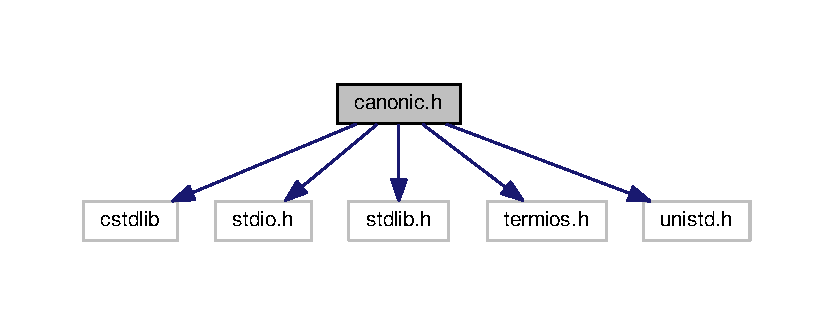
\includegraphics[width=350pt]{canonic_8h__incl}
\end{center}
\end{figure}
This graph shows which files directly or indirectly include this file\+:
\nopagebreak
\begin{figure}[H]
\begin{center}
\leavevmode
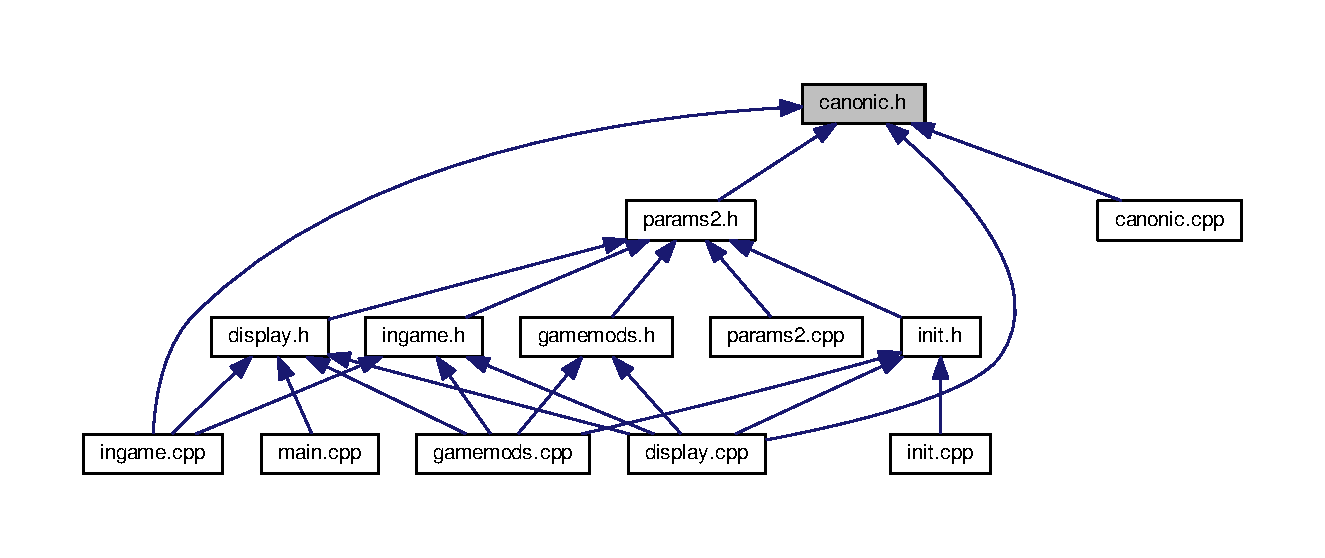
\includegraphics[width=350pt]{canonic_8h__dep__incl}
\end{center}
\end{figure}
\subsection*{Functions}
\begin{DoxyCompactItemize}
\item 
\hypertarget{canonic_8h_af99d8c0775d8c342a142e2be8c2ea592}{void \hyperlink{canonic_8h_af99d8c0775d8c342a142e2be8c2ea592}{reset\+\_\+input\+\_\+mode} (void)}\label{canonic_8h_af99d8c0775d8c342a142e2be8c2ea592}

\begin{DoxyCompactList}\small\item\em reset\+\_\+input\+\_\+mode permet le passage au mode canonique \end{DoxyCompactList}\item 
\hypertarget{canonic_8h_a224cd3d46cfe5381606415ce3585b91f}{void \hyperlink{canonic_8h_a224cd3d46cfe5381606415ce3585b91f}{set\+\_\+input\+\_\+mode} (void)}\label{canonic_8h_a224cd3d46cfe5381606415ce3585b91f}

\begin{DoxyCompactList}\small\item\em set\+\_\+input\+\_\+mode permet le passage au mode non canonique \end{DoxyCompactList}\end{DoxyCompactItemize}


\subsection{Detailed Description}
Passage du mode canonique à non canonique qui permet de rendre le jeu plus réactif. 

\begin{DoxyAuthor}{Author}
Quentin Pla, Léo Vincent, Emma tarfi, Sirine Achache, Julien Vavrille
\end{DoxyAuthor}
\begin{DoxyDate}{Date}
26 janvier 2018 
\end{DoxyDate}


Definition in file \hyperlink{canonic_8h_source}{canonic.\+h}.


\hypertarget{display_8h}{\section{display.\+h File Reference}
\label{display_8h}\index{display.\+h@{display.\+h}}
}


Affichage du jeu à l'écran.  


{\ttfamily \#include \char`\"{}params2.\+h\char`\"{}}\\*
Include dependency graph for display.\+h\+:
\nopagebreak
\begin{figure}[H]
\begin{center}
\leavevmode
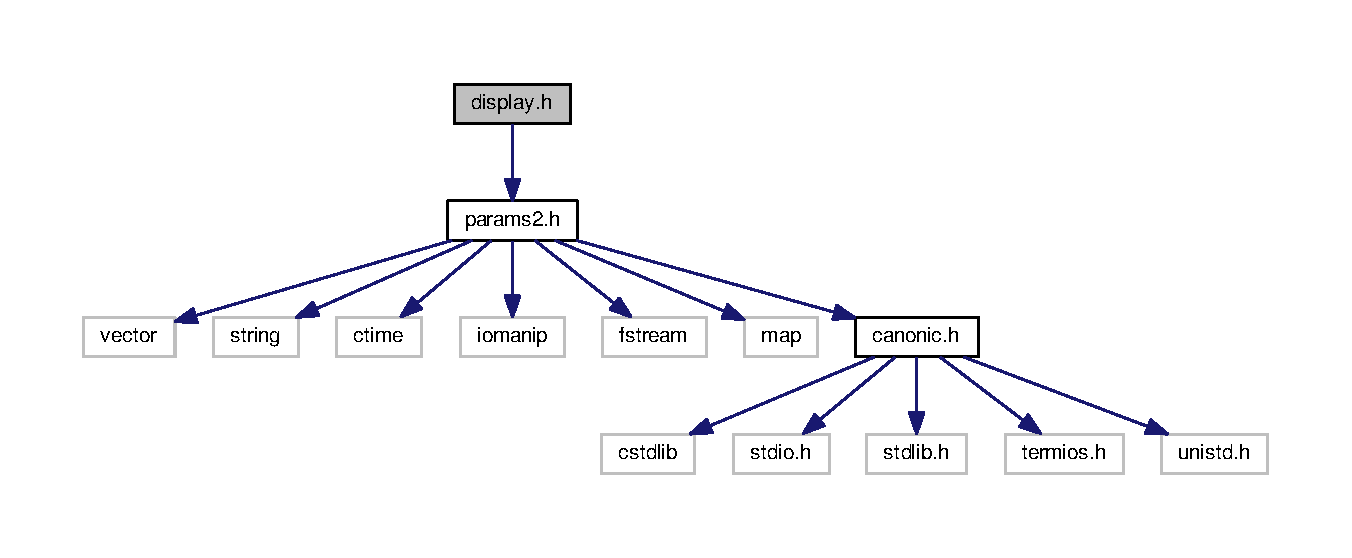
\includegraphics[width=350pt]{display_8h__incl}
\end{center}
\end{figure}
This graph shows which files directly or indirectly include this file\+:
\nopagebreak
\begin{figure}[H]
\begin{center}
\leavevmode
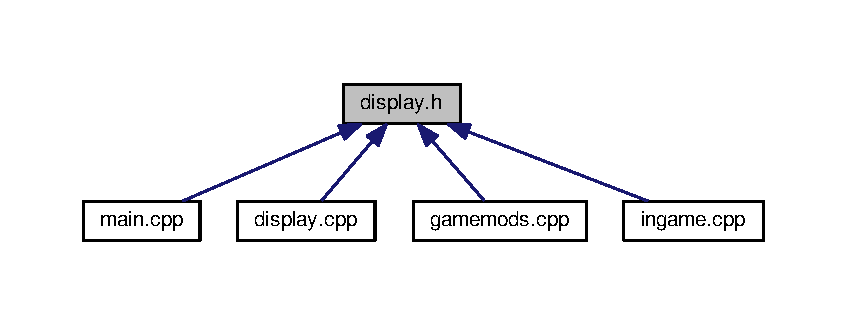
\includegraphics[width=350pt]{display_8h__dep__incl}
\end{center}
\end{figure}
\subsection*{Functions}
\begin{DoxyCompactItemize}
\item 
\hypertarget{display_8h_aa9714056a06d1518bdc6306412206580}{void \hyperlink{display_8h_aa9714056a06d1518bdc6306412206580}{Clear\+Screen2} ()}\label{display_8h_aa9714056a06d1518bdc6306412206580}

\begin{DoxyCompactList}\small\item\em Clear\+Screen2 efface l'écran. \end{DoxyCompactList}\item 
void \hyperlink{display_8h_a52d0ca86ff2a0ef127c0893799011754}{Display\+Window\+Borders} (unsigned Repeat)
\begin{DoxyCompactList}\small\item\em Display\+Window\+Borders affiche les bords de la fenêtre. \end{DoxyCompactList}\item 
void \hyperlink{display_8h_ac55c396e9d5a9409e1e6a7be81364f19}{Display\+Help\+Lines} (const C\+Mat \&Grid)
\begin{DoxyCompactList}\small\item\em Display\+Help\+Lines affiche les indices autour de la grille (de 1 à 9) \end{DoxyCompactList}\item 
void \hyperlink{display_8h_a1e6c116d2cd9c1b8ad9280fa2e200ca5}{Display\+Score} (int \&Score)
\begin{DoxyCompactList}\small\item\em Display\+Score affiche le score du joueur. \end{DoxyCompactList}\item 
void \hyperlink{display_8h_a5d48918d8cc1a3379e776d48dcdf2e2b}{Display\+Remaining\+Hits} (int \&Maximal\+Hits, int \&Hits)
\begin{DoxyCompactList}\small\item\em Display\+Remaining\+Hits affiche le nombre de coups restant. \end{DoxyCompactList}\item 
void \hyperlink{display_8h_a894fa592807b0958bf0e73d740452a62}{Display\+Leader\+Board} (const int \&Player\+Pos, const C\+Mat\+Str \&Leader\+Board, int \&Level\+Choice)
\begin{DoxyCompactList}\small\item\em Display\+Leader\+Board affiche le classement des meilleurs scores du 1er au 3e (affiche le nom du joueur et son score) \end{DoxyCompactList}\item 
void \hyperlink{display_8h_a39a7d88fa10d13a7ef05485a7b42dc67}{Display\+Stars} (int \&Score\+For\+Next\+Lvl, int \&Score)
\begin{DoxyCompactList}\small\item\em Display\+Stars affiche le pourcentage et les étoiles au dessus de la barre de progression (1er étoile = score atteind à 100\%, 2e à 150\% et 3e à 200\%) \end{DoxyCompactList}\item 
void \hyperlink{display_8h_a91eab476771d28a0752e85888d477f9b}{Display\+Progress\+Bar} (int \&Score\+For\+Next\+Lvl, int \&Score)
\begin{DoxyCompactList}\small\item\em Display\+Progress\+Bar affiche la barre de progression. \end{DoxyCompactList}\item 
\hypertarget{display_8h_a6c3c37c60f48772ed93ef51a142f0dc8}{void \hyperlink{display_8h_a6c3c37c60f48772ed93ef51a142f0dc8}{Display\+Header} ()}\label{display_8h_a6c3c37c60f48772ed93ef51a142f0dc8}

\begin{DoxyCompactList}\small\item\em Display\+Header affiche la partie haute de la fenêtre contenant \char`\"{}\+N\+U\+M\+B\+E\+R C\+R\+U\+S\+H\char`\"{}. \end{DoxyCompactList}\item 
void \hyperlink{display_8h_a985915bc685c3aa57c3b75c4720b071f}{Display\+Window} (const C\+Mat \&Grid, const C\+Mat\+Str \&Leader\+Board, int \&Score\+For\+Next\+Lvl, int \&Score, int \&Level\+Choice, int \&Maximal\+Hits, int \&Hits)
\begin{DoxyCompactList}\small\item\em Display\+Window affiche la grille et tout le reste de la fenêtre en appelant chaque fonctions indépendamment. \end{DoxyCompactList}\item 
void \hyperlink{display_8h_ab77f0cd8eb631a2675c55cbb24bc4fee}{Game\+Over} (const string \&Pseudo)
\begin{DoxyCompactList}\small\item\em Game\+Over affiche la fenêtre \char`\"{}\+G\+A\+M\+E O\+V\+E\+R\char`\"{} lorsque le joueur a perdu. \end{DoxyCompactList}\item 
void \hyperlink{display_8h_a2136d186fc0e7a3e00be122068e5810c}{Win\+Game} (const string \&Pseudo)
\begin{DoxyCompactList}\small\item\em Win\+Game affiche la fenêtre \char`\"{}\+Y\+O\+U W\+I\+N\char`\"{} lorsque le joueur a gagné \end{DoxyCompactList}\item 
void \hyperlink{display_8h_ae89e5a96380a3c5e6d8c198020696084}{Show\+Menu} (const string \&Pseudo)
\begin{DoxyCompactList}\small\item\em Show\+Menu affiche le menu de sélection du mode de jeu (choix entre C\+L\+A\+S\+S\+I\+C, D\+I\+A\+G\+O\+N\+A\+L, R\+U\+L\+E\+S) \end{DoxyCompactList}\item 
void \hyperlink{display_8h_a5a4378a081a78a48ba12ec54a6a1a299}{Show\+Rules} (const string \&Pseudo)
\begin{DoxyCompactList}\small\item\em Show\+Rules affiche les régles des différents modes de jeu ainsi que les actions définies pour chaque touche. \end{DoxyCompactList}\item 
\hypertarget{display_8h_ad2f3df7bd5ff146b699003a5d7bdfd7c}{void \hyperlink{display_8h_ad2f3df7bd5ff146b699003a5d7bdfd7c}{Connexion} ()}\label{display_8h_ad2f3df7bd5ff146b699003a5d7bdfd7c}

\begin{DoxyCompactList}\small\item\em Connexion affiche la page de connexion où le joueur se connecte avec son pseudo. \end{DoxyCompactList}\item 
void \hyperlink{display_8h_a8084e88f83b951438d2d556697b62260}{Show\+Levels} (C\+Mat \&Grid, int \&Score\+For\+Next\+Lvl, int \&Level\+Choice, int \&Maximal\+Hits, const string \&Pseudo)
\begin{DoxyCompactList}\small\item\em Show\+Levels affiche les différents niveaux disponibles pour chaque mode de jeu. \end{DoxyCompactList}\end{DoxyCompactItemize}


\subsection{Detailed Description}
Affichage du jeu à l'écran. 

\begin{DoxyAuthor}{Author}
Quentin Pla, Léo Vincent, Emma tarfi, Sirine Achache, Julien Vavrille
\end{DoxyAuthor}
\begin{DoxyDate}{Date}
26 janvier 2018 
\end{DoxyDate}


Definition in file \hyperlink{display_8h_source}{display.\+h}.



\subsection{Function Documentation}
\hypertarget{display_8h_ac55c396e9d5a9409e1e6a7be81364f19}{\index{display.\+h@{display.\+h}!Display\+Help\+Lines@{Display\+Help\+Lines}}
\index{Display\+Help\+Lines@{Display\+Help\+Lines}!display.\+h@{display.\+h}}
\subsubsection[{Display\+Help\+Lines}]{\setlength{\rightskip}{0pt plus 5cm}void Display\+Help\+Lines (
\begin{DoxyParamCaption}
\item[{const C\+Mat \&}]{Grid}
\end{DoxyParamCaption}
)}}\label{display_8h_ac55c396e9d5a9409e1e6a7be81364f19}


Display\+Help\+Lines affiche les indices autour de la grille (de 1 à 9) 


\begin{DoxyParams}{Parameters}
{\em Grid\mbox{[}in\mbox{]}} & Grille contenant les nombres \\
\hline
\end{DoxyParams}


Definition at line 29 of file display.\+cpp.



Here is the caller graph for this function\+:
\nopagebreak
\begin{figure}[H]
\begin{center}
\leavevmode
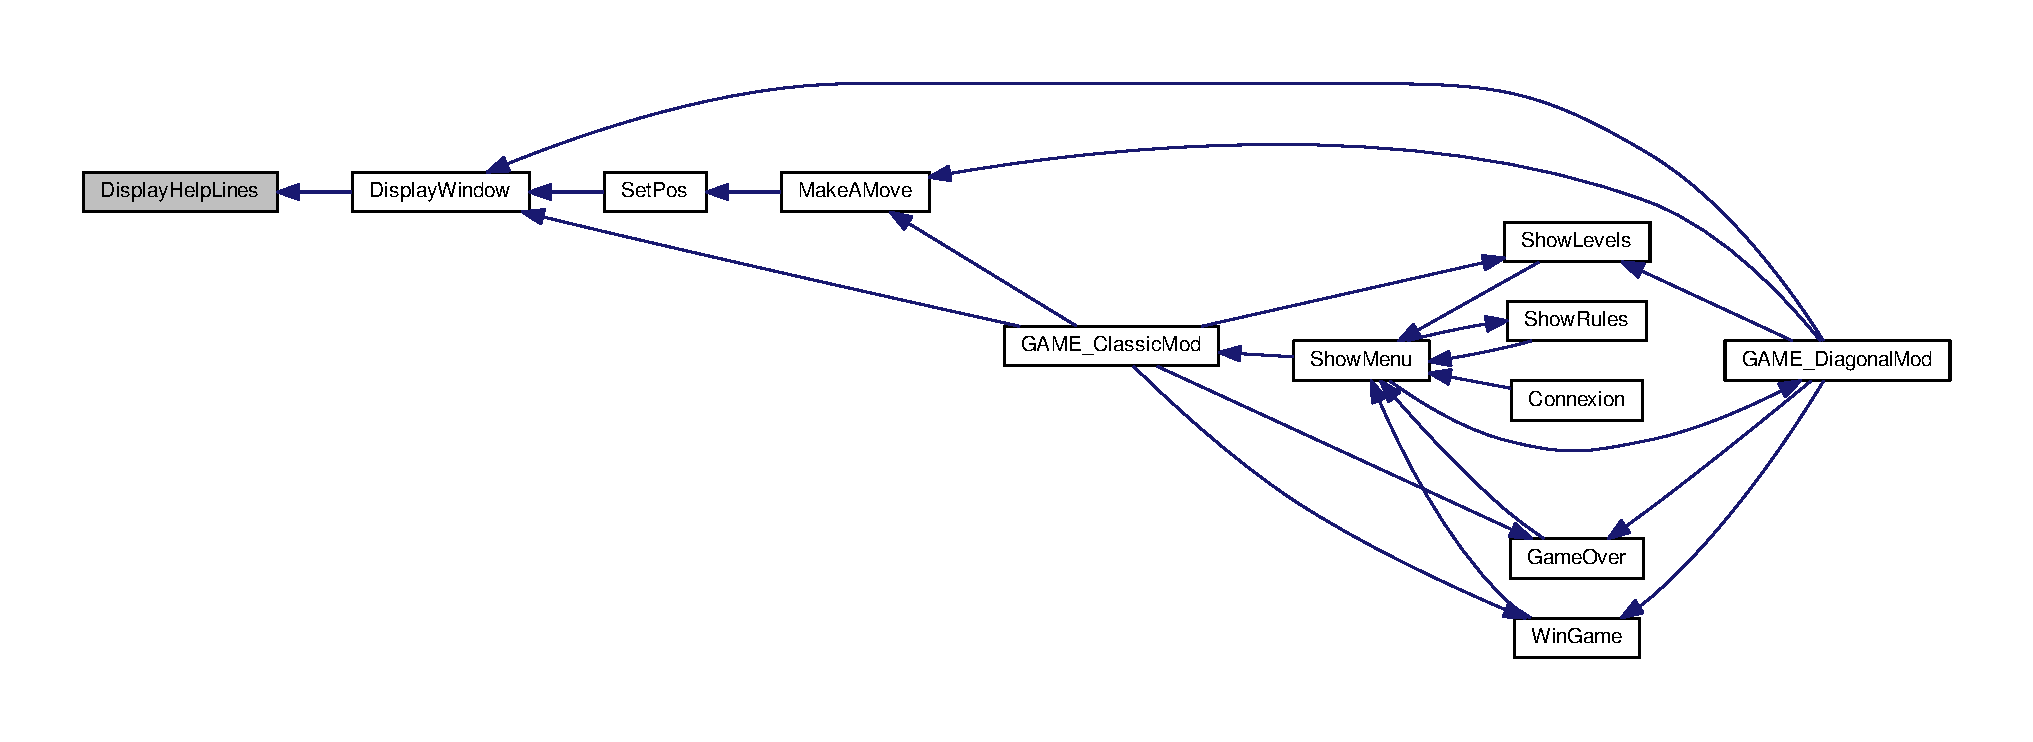
\includegraphics[width=350pt]{display_8h_ac55c396e9d5a9409e1e6a7be81364f19_icgraph}
\end{center}
\end{figure}


\hypertarget{display_8h_a894fa592807b0958bf0e73d740452a62}{\index{display.\+h@{display.\+h}!Display\+Leader\+Board@{Display\+Leader\+Board}}
\index{Display\+Leader\+Board@{Display\+Leader\+Board}!display.\+h@{display.\+h}}
\subsubsection[{Display\+Leader\+Board}]{\setlength{\rightskip}{0pt plus 5cm}void Display\+Leader\+Board (
\begin{DoxyParamCaption}
\item[{const int \&}]{Player\+Pos, }
\item[{const C\+Mat\+Str \&}]{Leader\+Board, }
\item[{int \&}]{Level\+Choice}
\end{DoxyParamCaption}
)}}\label{display_8h_a894fa592807b0958bf0e73d740452a62}


Display\+Leader\+Board affiche le classement des meilleurs scores du 1er au 3e (affiche le nom du joueur et son score) 


\begin{DoxyParams}{Parameters}
{\em Player\+Pos\mbox{[}in\mbox{]}} & Ligne à afficher du classement (de 0 à 4) \\
\hline
{\em Leader\+Board\mbox{[}in\mbox{]}} & Matrice contenant l'ensemble des scores des joueurs pour chaque niveau \\
\hline
{\em Level\+Choice\mbox{[}in\mbox{]}} & Niveau sélectionné \\
\hline
\end{DoxyParams}


Definition at line 50 of file display.\+cpp.



Here is the caller graph for this function\+:
\nopagebreak
\begin{figure}[H]
\begin{center}
\leavevmode
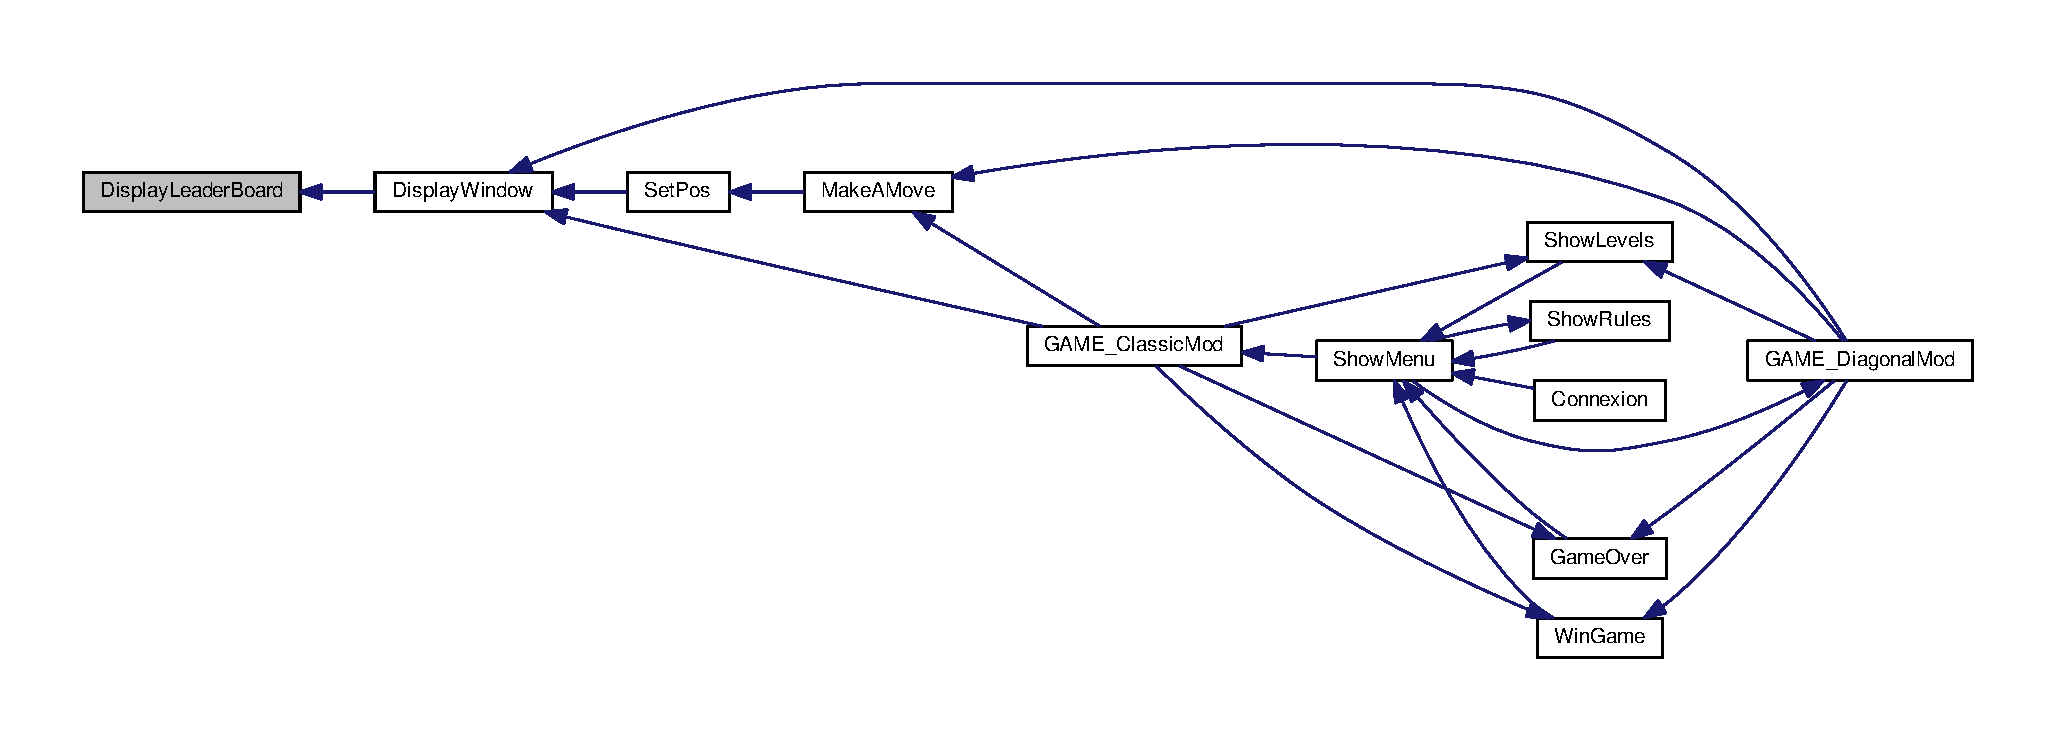
\includegraphics[width=350pt]{display_8h_a894fa592807b0958bf0e73d740452a62_icgraph}
\end{center}
\end{figure}


\hypertarget{display_8h_a91eab476771d28a0752e85888d477f9b}{\index{display.\+h@{display.\+h}!Display\+Progress\+Bar@{Display\+Progress\+Bar}}
\index{Display\+Progress\+Bar@{Display\+Progress\+Bar}!display.\+h@{display.\+h}}
\subsubsection[{Display\+Progress\+Bar}]{\setlength{\rightskip}{0pt plus 5cm}void Display\+Progress\+Bar (
\begin{DoxyParamCaption}
\item[{int \&}]{Score\+For\+Next\+Lvl, }
\item[{int \&}]{Score}
\end{DoxyParamCaption}
)}}\label{display_8h_a91eab476771d28a0752e85888d477f9b}


Display\+Progress\+Bar affiche la barre de progression. 


\begin{DoxyParams}{Parameters}
{\em Score\+For\+Next\+Lvl\mbox{[}in\mbox{]}} & Score à atteindre pour gagner le niveau \\
\hline
{\em Score\mbox{[}in\mbox{]}} & Score du joueur \\
\hline
\end{DoxyParams}


Definition at line 76 of file display.\+cpp.



Here is the call graph for this function\+:
\nopagebreak
\begin{figure}[H]
\begin{center}
\leavevmode
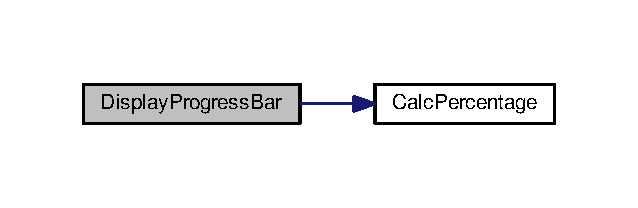
\includegraphics[width=306pt]{display_8h_a91eab476771d28a0752e85888d477f9b_cgraph}
\end{center}
\end{figure}




Here is the caller graph for this function\+:
\nopagebreak
\begin{figure}[H]
\begin{center}
\leavevmode
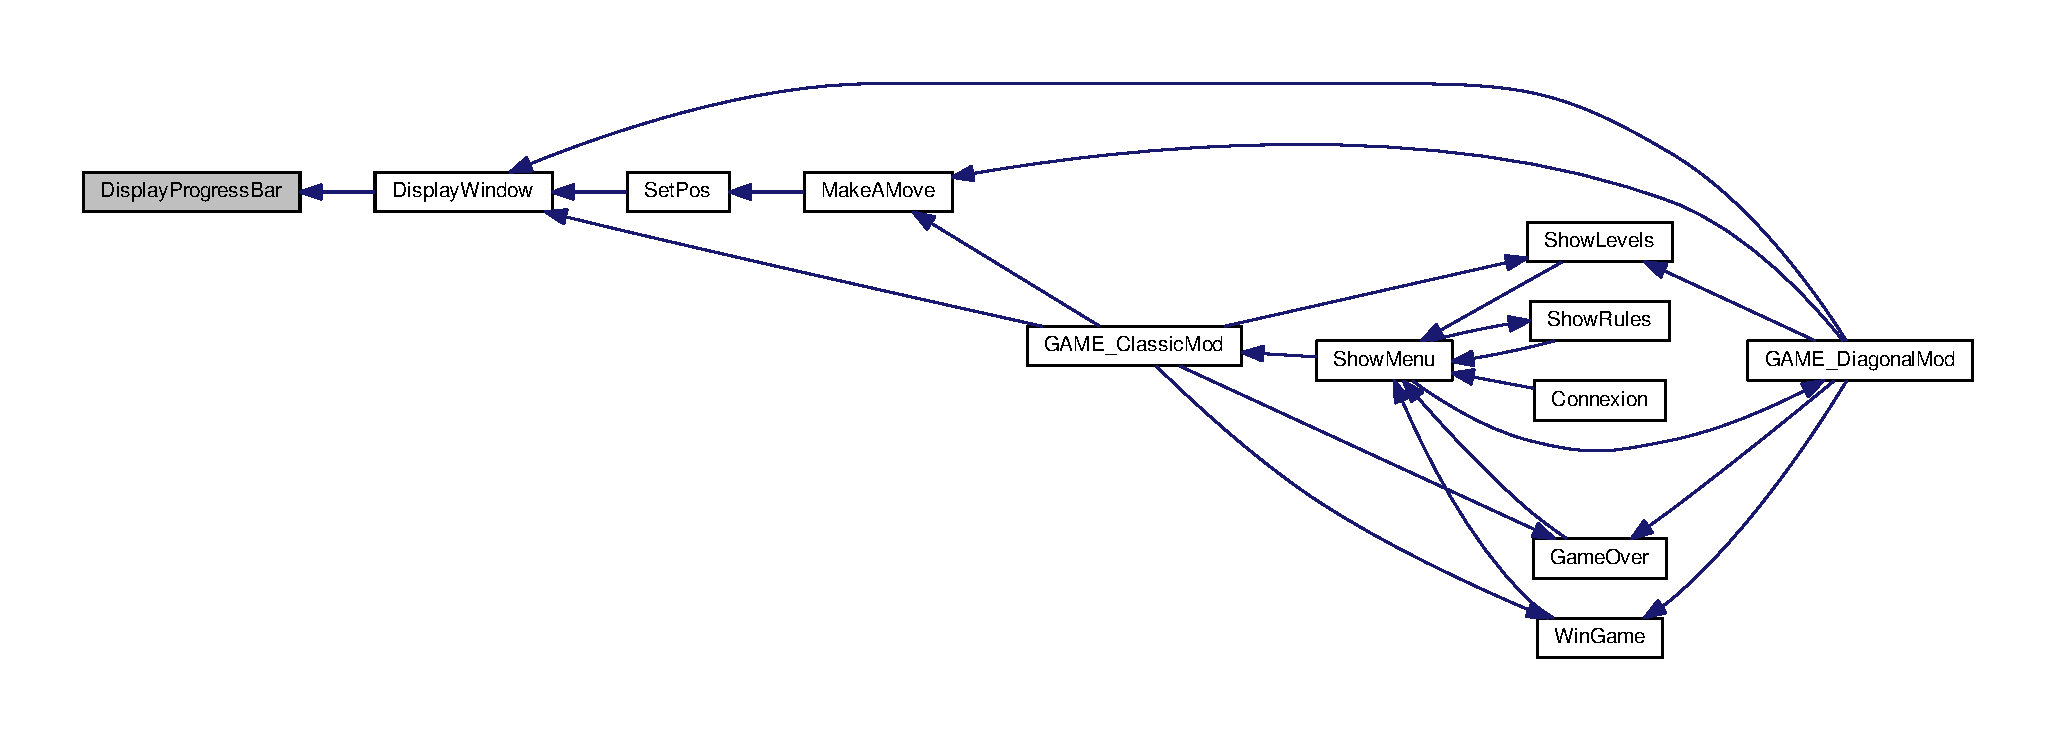
\includegraphics[width=350pt]{display_8h_a91eab476771d28a0752e85888d477f9b_icgraph}
\end{center}
\end{figure}


\hypertarget{display_8h_a5d48918d8cc1a3379e776d48dcdf2e2b}{\index{display.\+h@{display.\+h}!Display\+Remaining\+Hits@{Display\+Remaining\+Hits}}
\index{Display\+Remaining\+Hits@{Display\+Remaining\+Hits}!display.\+h@{display.\+h}}
\subsubsection[{Display\+Remaining\+Hits}]{\setlength{\rightskip}{0pt plus 5cm}void Display\+Remaining\+Hits (
\begin{DoxyParamCaption}
\item[{int \&}]{Maximal\+Hits, }
\item[{int \&}]{Hits}
\end{DoxyParamCaption}
)}}\label{display_8h_a5d48918d8cc1a3379e776d48dcdf2e2b}


Display\+Remaining\+Hits affiche le nombre de coups restant. 


\begin{DoxyParams}{Parameters}
{\em Maximal\+Hits\mbox{[}in\mbox{]}} & Nombre maximum de coups attribués pour le level \\
\hline
{\em Hits\mbox{[}in\mbox{]}} & Nombre de coups utilisés \\
\hline
\end{DoxyParams}


Definition at line 45 of file display.\+cpp.



Here is the caller graph for this function\+:
\nopagebreak
\begin{figure}[H]
\begin{center}
\leavevmode
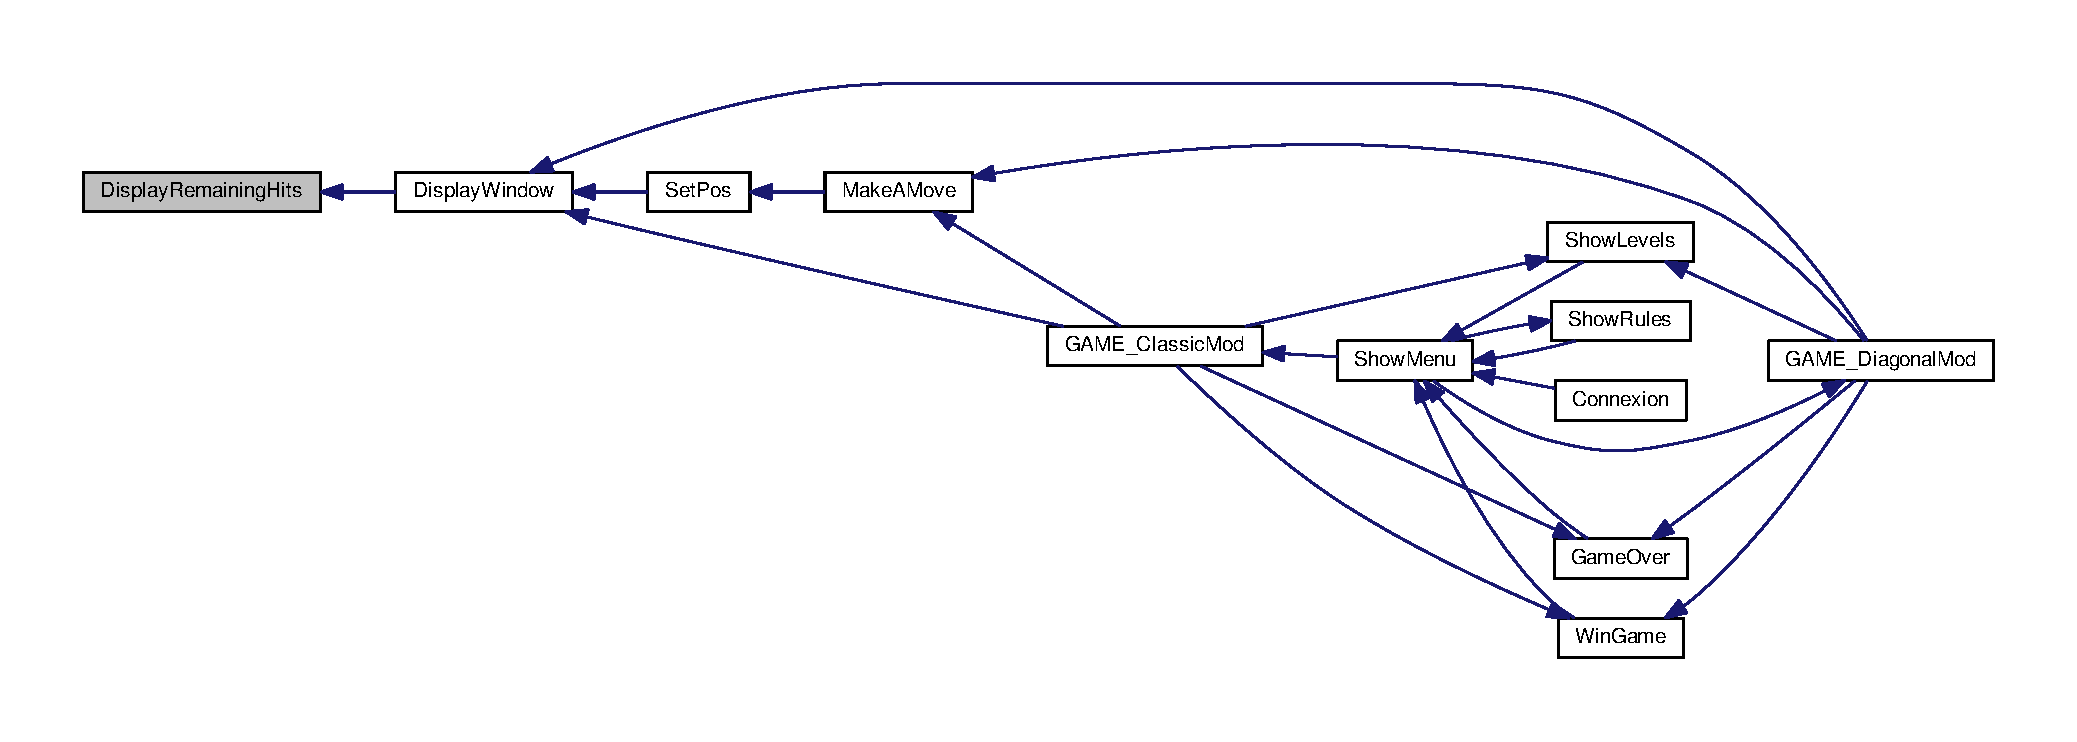
\includegraphics[width=350pt]{display_8h_a5d48918d8cc1a3379e776d48dcdf2e2b_icgraph}
\end{center}
\end{figure}


\hypertarget{display_8h_a1e6c116d2cd9c1b8ad9280fa2e200ca5}{\index{display.\+h@{display.\+h}!Display\+Score@{Display\+Score}}
\index{Display\+Score@{Display\+Score}!display.\+h@{display.\+h}}
\subsubsection[{Display\+Score}]{\setlength{\rightskip}{0pt plus 5cm}void Display\+Score (
\begin{DoxyParamCaption}
\item[{int \&}]{Score}
\end{DoxyParamCaption}
)}}\label{display_8h_a1e6c116d2cd9c1b8ad9280fa2e200ca5}


Display\+Score affiche le score du joueur. 


\begin{DoxyParams}{Parameters}
{\em Score\mbox{[}in\mbox{]}} & Score du joueur \\
\hline
\end{DoxyParams}


Definition at line 40 of file display.\+cpp.



Here is the caller graph for this function\+:
\nopagebreak
\begin{figure}[H]
\begin{center}
\leavevmode
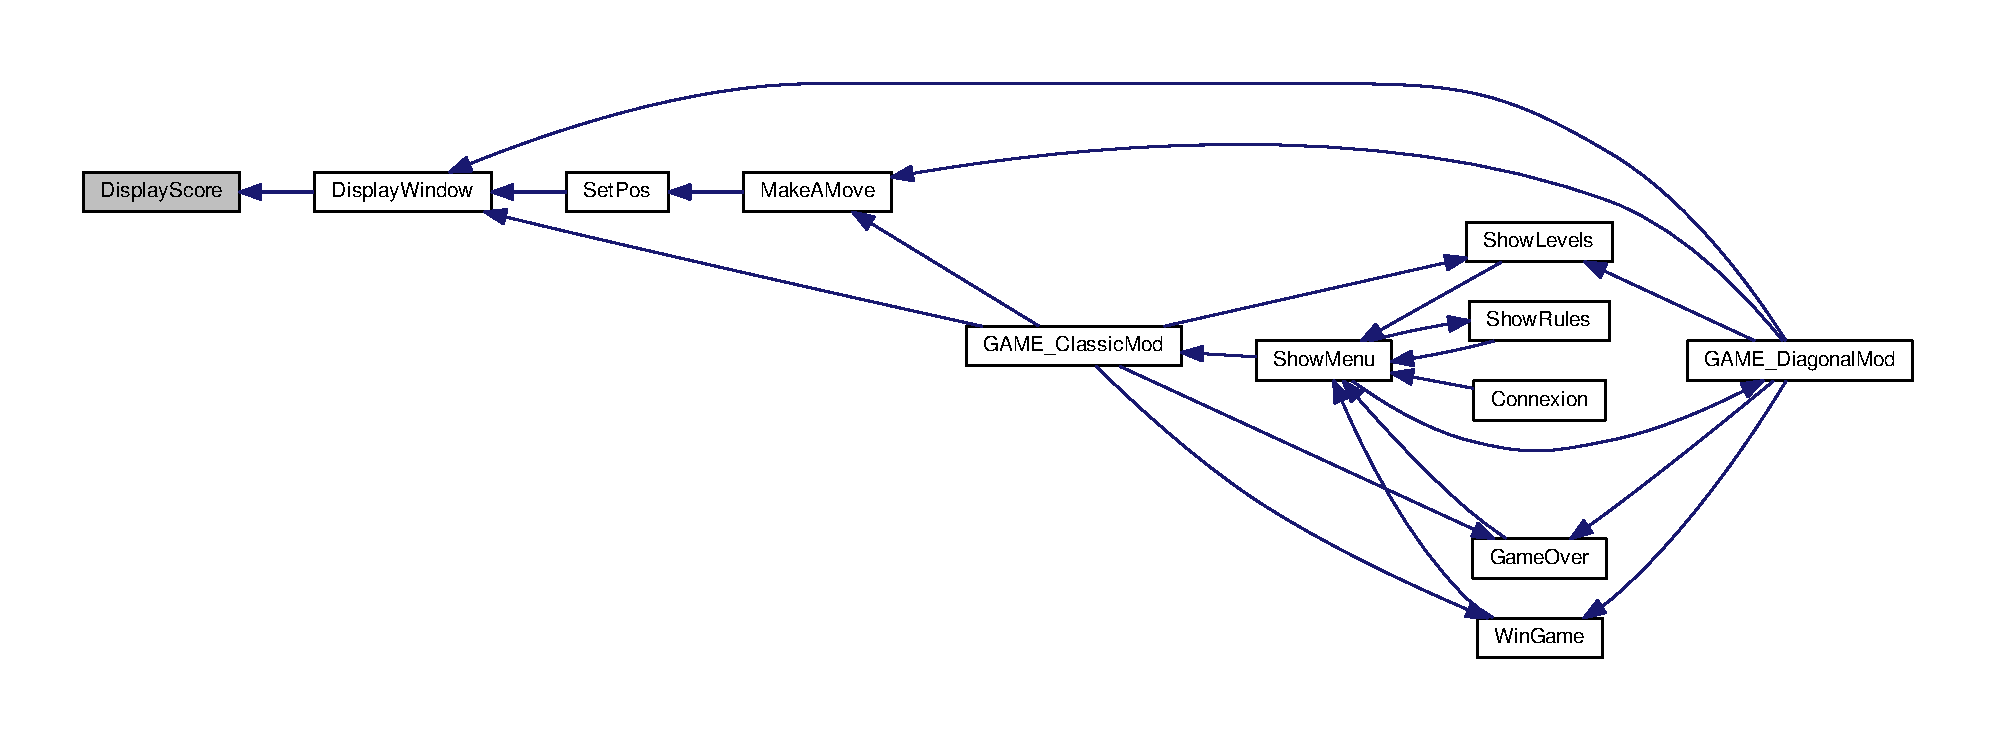
\includegraphics[width=350pt]{display_8h_a1e6c116d2cd9c1b8ad9280fa2e200ca5_icgraph}
\end{center}
\end{figure}


\hypertarget{display_8h_a39a7d88fa10d13a7ef05485a7b42dc67}{\index{display.\+h@{display.\+h}!Display\+Stars@{Display\+Stars}}
\index{Display\+Stars@{Display\+Stars}!display.\+h@{display.\+h}}
\subsubsection[{Display\+Stars}]{\setlength{\rightskip}{0pt plus 5cm}void Display\+Stars (
\begin{DoxyParamCaption}
\item[{int \&}]{Score\+For\+Next\+Lvl, }
\item[{int \&}]{Score}
\end{DoxyParamCaption}
)}}\label{display_8h_a39a7d88fa10d13a7ef05485a7b42dc67}


Display\+Stars affiche le pourcentage et les étoiles au dessus de la barre de progression (1er étoile = score atteind à 100\%, 2e à 150\% et 3e à 200\%) 


\begin{DoxyParams}{Parameters}
{\em Score\+For\+Next\+Lvl\mbox{[}in\mbox{]}} & Score à atteindre pour gagner le niveau \\
\hline
{\em Score\mbox{[}in\mbox{]}} & Score du joueur \\
\hline
\end{DoxyParams}


Definition at line 63 of file display.\+cpp.



Here is the call graph for this function\+:
\nopagebreak
\begin{figure}[H]
\begin{center}
\leavevmode
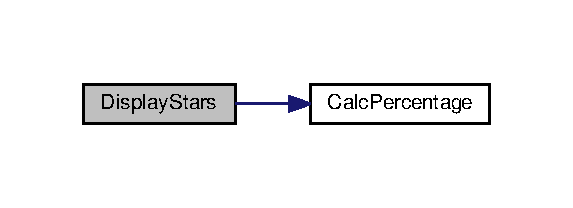
\includegraphics[width=275pt]{display_8h_a39a7d88fa10d13a7ef05485a7b42dc67_cgraph}
\end{center}
\end{figure}




Here is the caller graph for this function\+:
\nopagebreak
\begin{figure}[H]
\begin{center}
\leavevmode
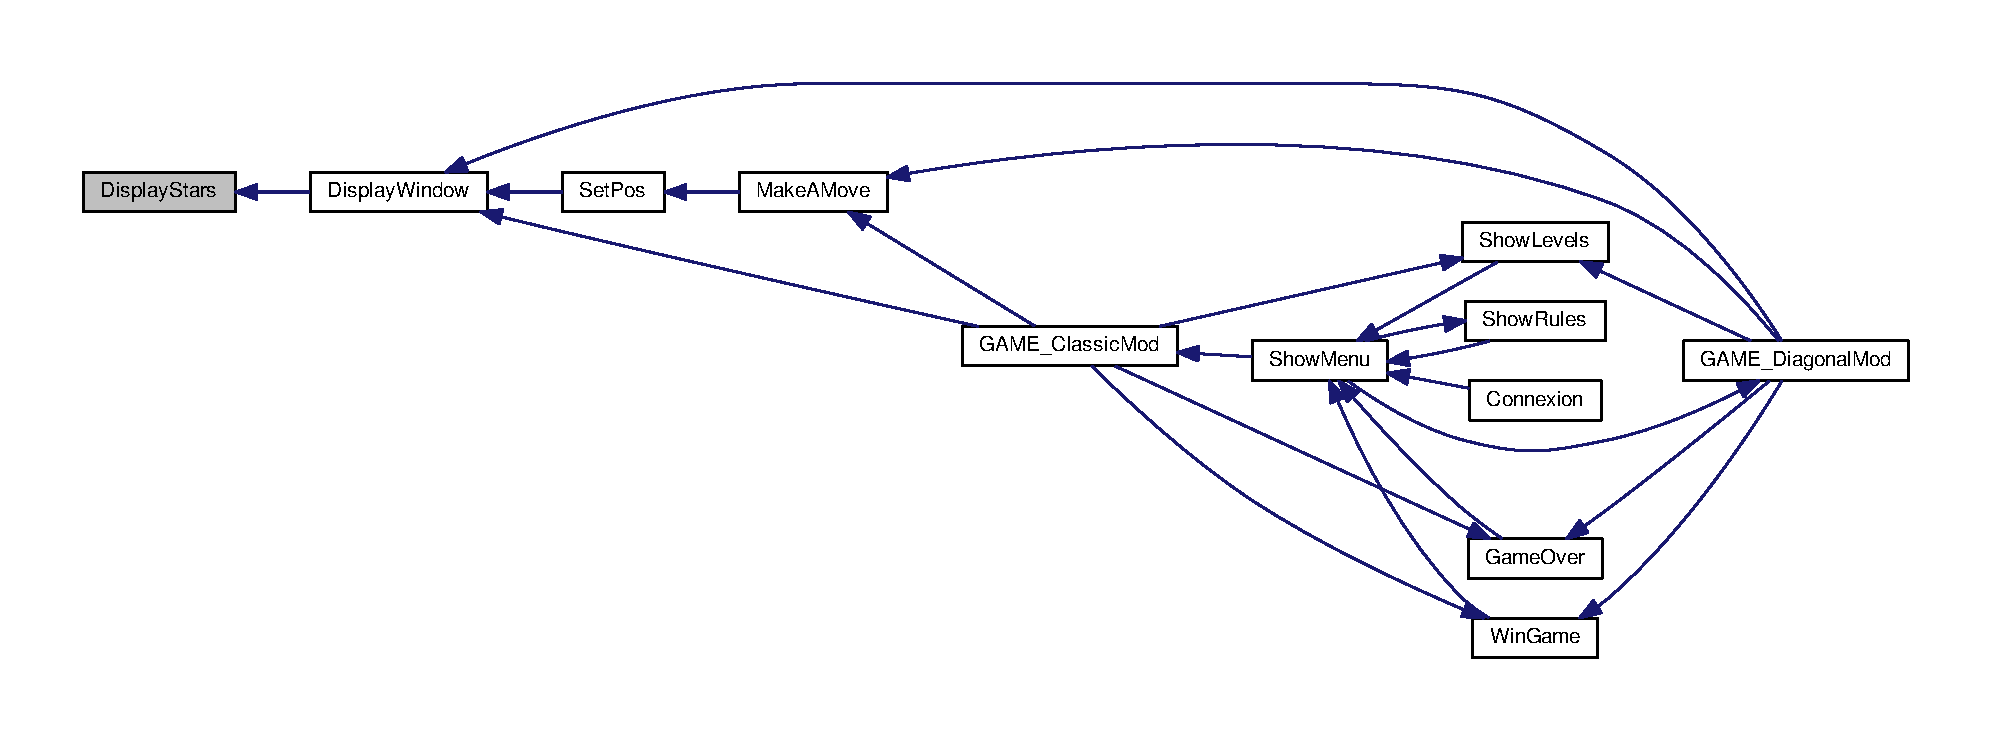
\includegraphics[width=350pt]{display_8h_a39a7d88fa10d13a7ef05485a7b42dc67_icgraph}
\end{center}
\end{figure}


\hypertarget{display_8h_a985915bc685c3aa57c3b75c4720b071f}{\index{display.\+h@{display.\+h}!Display\+Window@{Display\+Window}}
\index{Display\+Window@{Display\+Window}!display.\+h@{display.\+h}}
\subsubsection[{Display\+Window}]{\setlength{\rightskip}{0pt plus 5cm}void Display\+Window (
\begin{DoxyParamCaption}
\item[{const C\+Mat \&}]{Grid, }
\item[{const C\+Mat\+Str \&}]{Leader\+Board, }
\item[{int \&}]{Score\+For\+Next\+Lvl, }
\item[{int \&}]{Score, }
\item[{int \&}]{Level\+Choice, }
\item[{int \&}]{Maximal\+Hits, }
\item[{int \&}]{Hits}
\end{DoxyParamCaption}
)}}\label{display_8h_a985915bc685c3aa57c3b75c4720b071f}


Display\+Window affiche la grille et tout le reste de la fenêtre en appelant chaque fonctions indépendamment. 


\begin{DoxyParams}{Parameters}
{\em Grid\mbox{[}in\mbox{]}} & Grille contenant les nombres \\
\hline
{\em Leader\+Board\mbox{[}in\mbox{]}} & Matrice contenant l'ensemble des scores des joueurs pour chaque niveau \\
\hline
{\em Score\+For\+Next\+Lvl\mbox{[}in\mbox{]}} & Score à atteindre pour gagner le niveau \\
\hline
{\em Score\mbox{[}in\mbox{]}} & Score du joueur \\
\hline
{\em Level\+Choice\mbox{[}in\mbox{]}} & Level choisi par l'utilisateur \\
\hline
{\em Maximal\+Hits\mbox{[}in\mbox{]}} & Nombre maximum de coups attribués pour le level \\
\hline
{\em Hits\mbox{[}in\mbox{]}} & Nombre de coups utilisés \\
\hline
\end{DoxyParams}


Definition at line 98 of file display.\+cpp.



Here is the call graph for this function\+:
\nopagebreak
\begin{figure}[H]
\begin{center}
\leavevmode
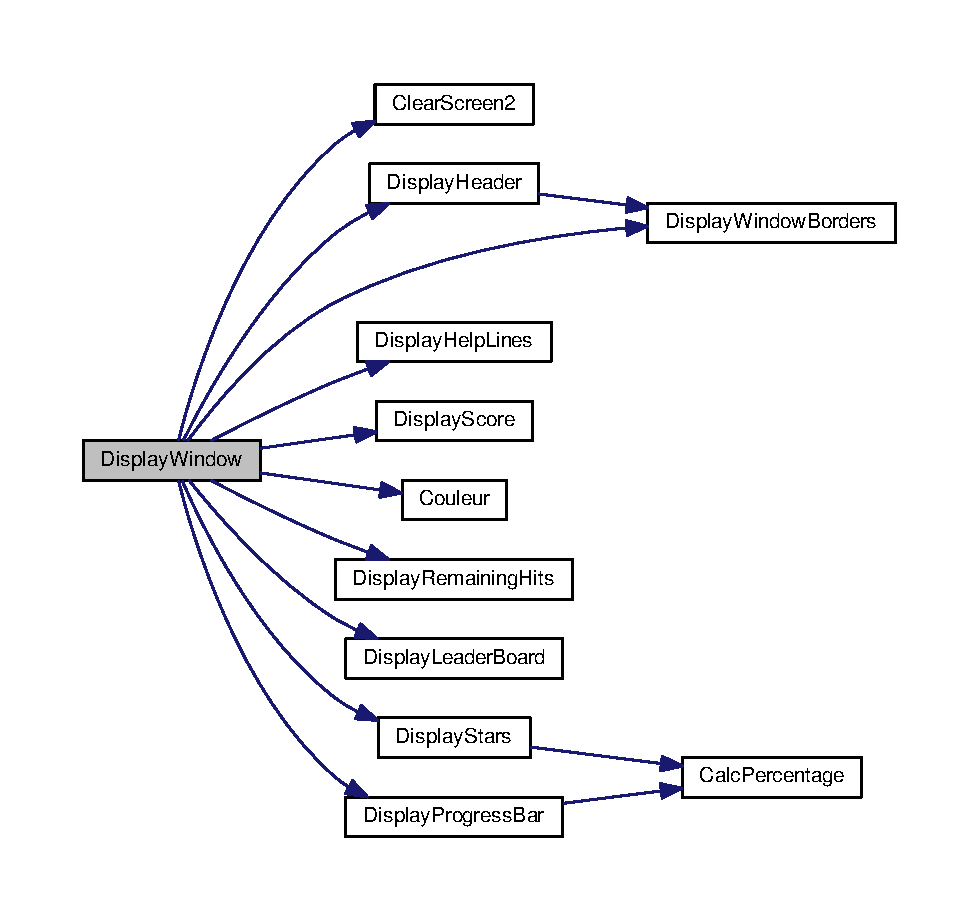
\includegraphics[width=350pt]{display_8h_a985915bc685c3aa57c3b75c4720b071f_cgraph}
\end{center}
\end{figure}




Here is the caller graph for this function\+:
\nopagebreak
\begin{figure}[H]
\begin{center}
\leavevmode
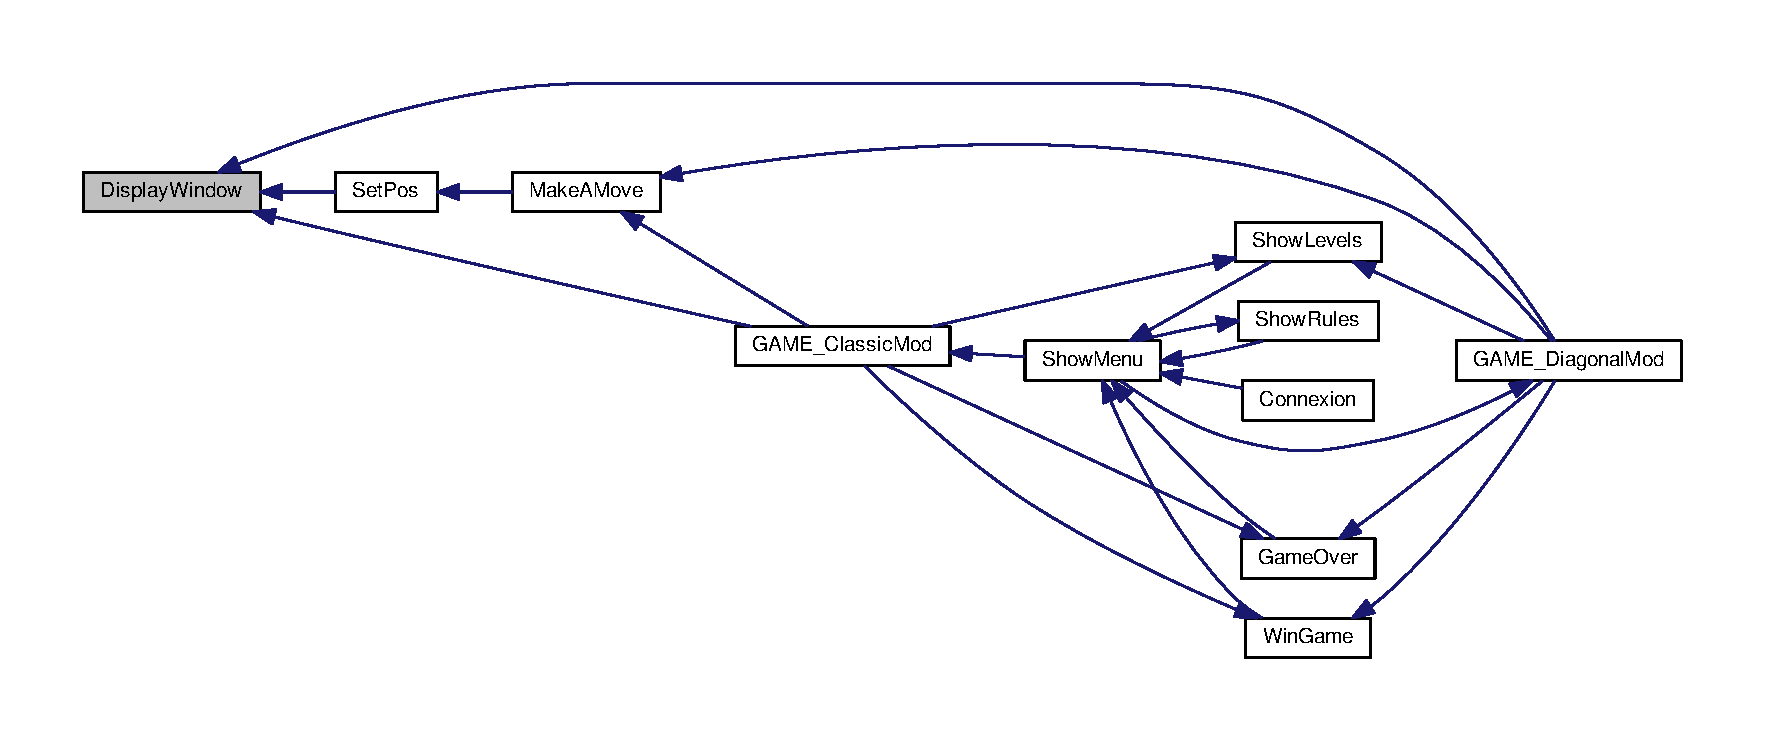
\includegraphics[width=350pt]{display_8h_a985915bc685c3aa57c3b75c4720b071f_icgraph}
\end{center}
\end{figure}


\hypertarget{display_8h_a52d0ca86ff2a0ef127c0893799011754}{\index{display.\+h@{display.\+h}!Display\+Window\+Borders@{Display\+Window\+Borders}}
\index{Display\+Window\+Borders@{Display\+Window\+Borders}!display.\+h@{display.\+h}}
\subsubsection[{Display\+Window\+Borders}]{\setlength{\rightskip}{0pt plus 5cm}void Display\+Window\+Borders (
\begin{DoxyParamCaption}
\item[{unsigned}]{Repeat}
\end{DoxyParamCaption}
)}}\label{display_8h_a52d0ca86ff2a0ef127c0893799011754}


Display\+Window\+Borders affiche les bords de la fenêtre. 


\begin{DoxyParams}{Parameters}
{\em Repeat\mbox{[}in\mbox{]}} & Nombre de répétitions pour l'affichage des bords \\
\hline
\end{DoxyParams}


Definition at line 20 of file display.\+cpp.



Here is the caller graph for this function\+:
\nopagebreak
\begin{figure}[H]
\begin{center}
\leavevmode
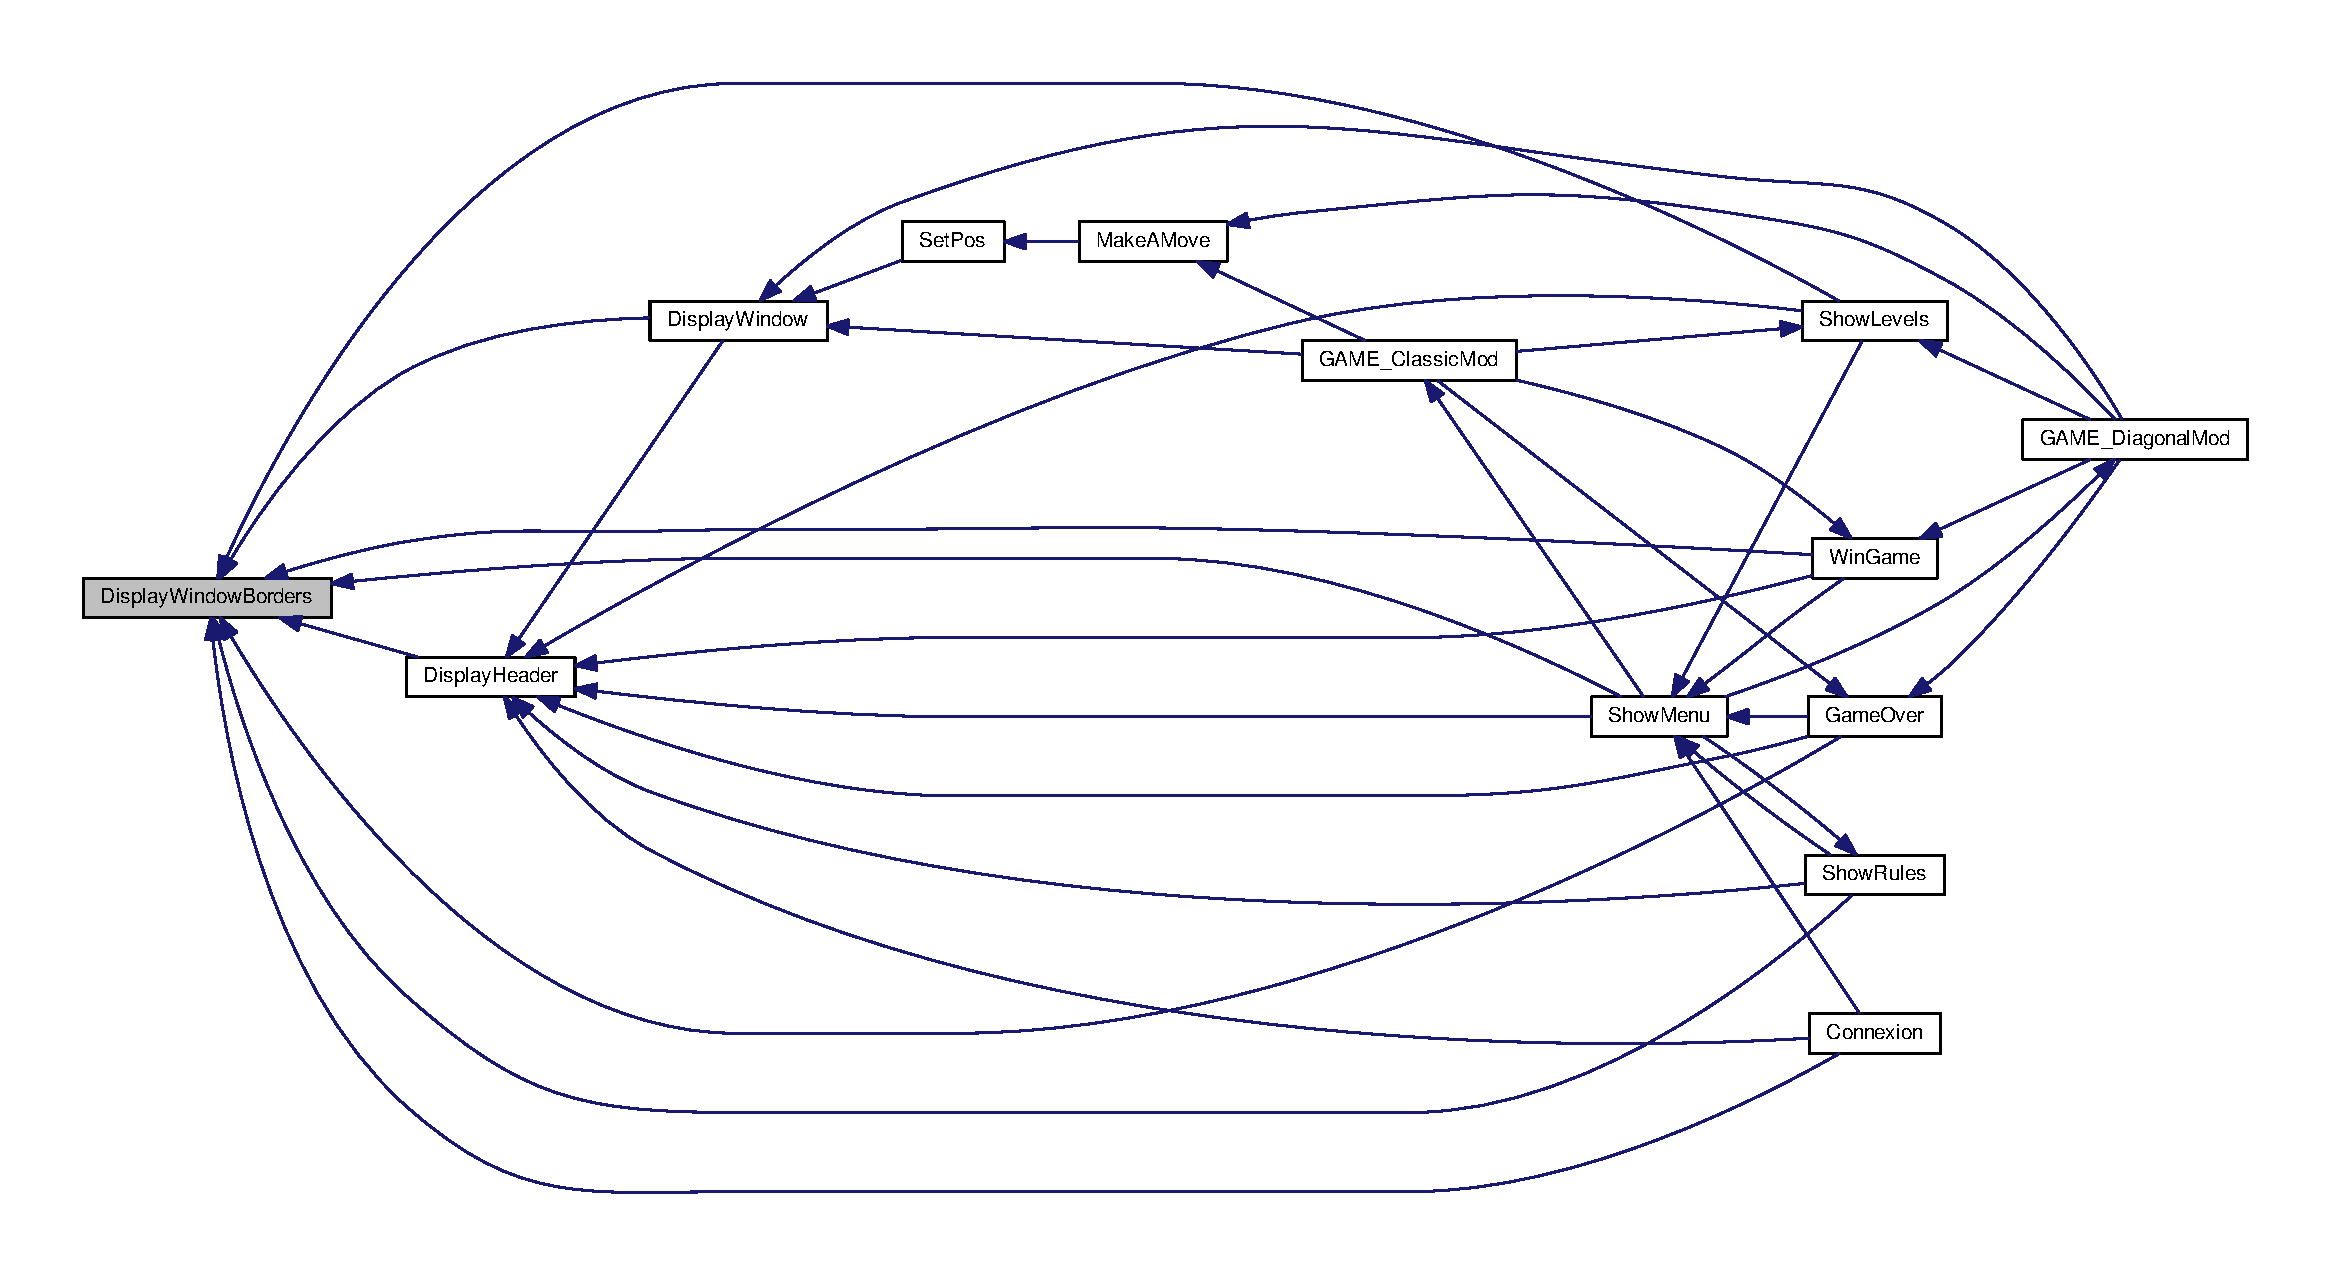
\includegraphics[width=350pt]{display_8h_a52d0ca86ff2a0ef127c0893799011754_icgraph}
\end{center}
\end{figure}


\hypertarget{display_8h_ab77f0cd8eb631a2675c55cbb24bc4fee}{\index{display.\+h@{display.\+h}!Game\+Over@{Game\+Over}}
\index{Game\+Over@{Game\+Over}!display.\+h@{display.\+h}}
\subsubsection[{Game\+Over}]{\setlength{\rightskip}{0pt plus 5cm}void Game\+Over (
\begin{DoxyParamCaption}
\item[{const string \&}]{Pseudo}
\end{DoxyParamCaption}
)}}\label{display_8h_ab77f0cd8eb631a2675c55cbb24bc4fee}


Game\+Over affiche la fenêtre \char`\"{}\+G\+A\+M\+E O\+V\+E\+R\char`\"{} lorsque le joueur a perdu. 


\begin{DoxyParams}{Parameters}
{\em Pseudo\mbox{[}in\mbox{]}} & Pseudo du joueur entré au début du jeu \\
\hline
\end{DoxyParams}


Definition at line 143 of file display.\+cpp.



Here is the call graph for this function\+:
\nopagebreak
\begin{figure}[H]
\begin{center}
\leavevmode
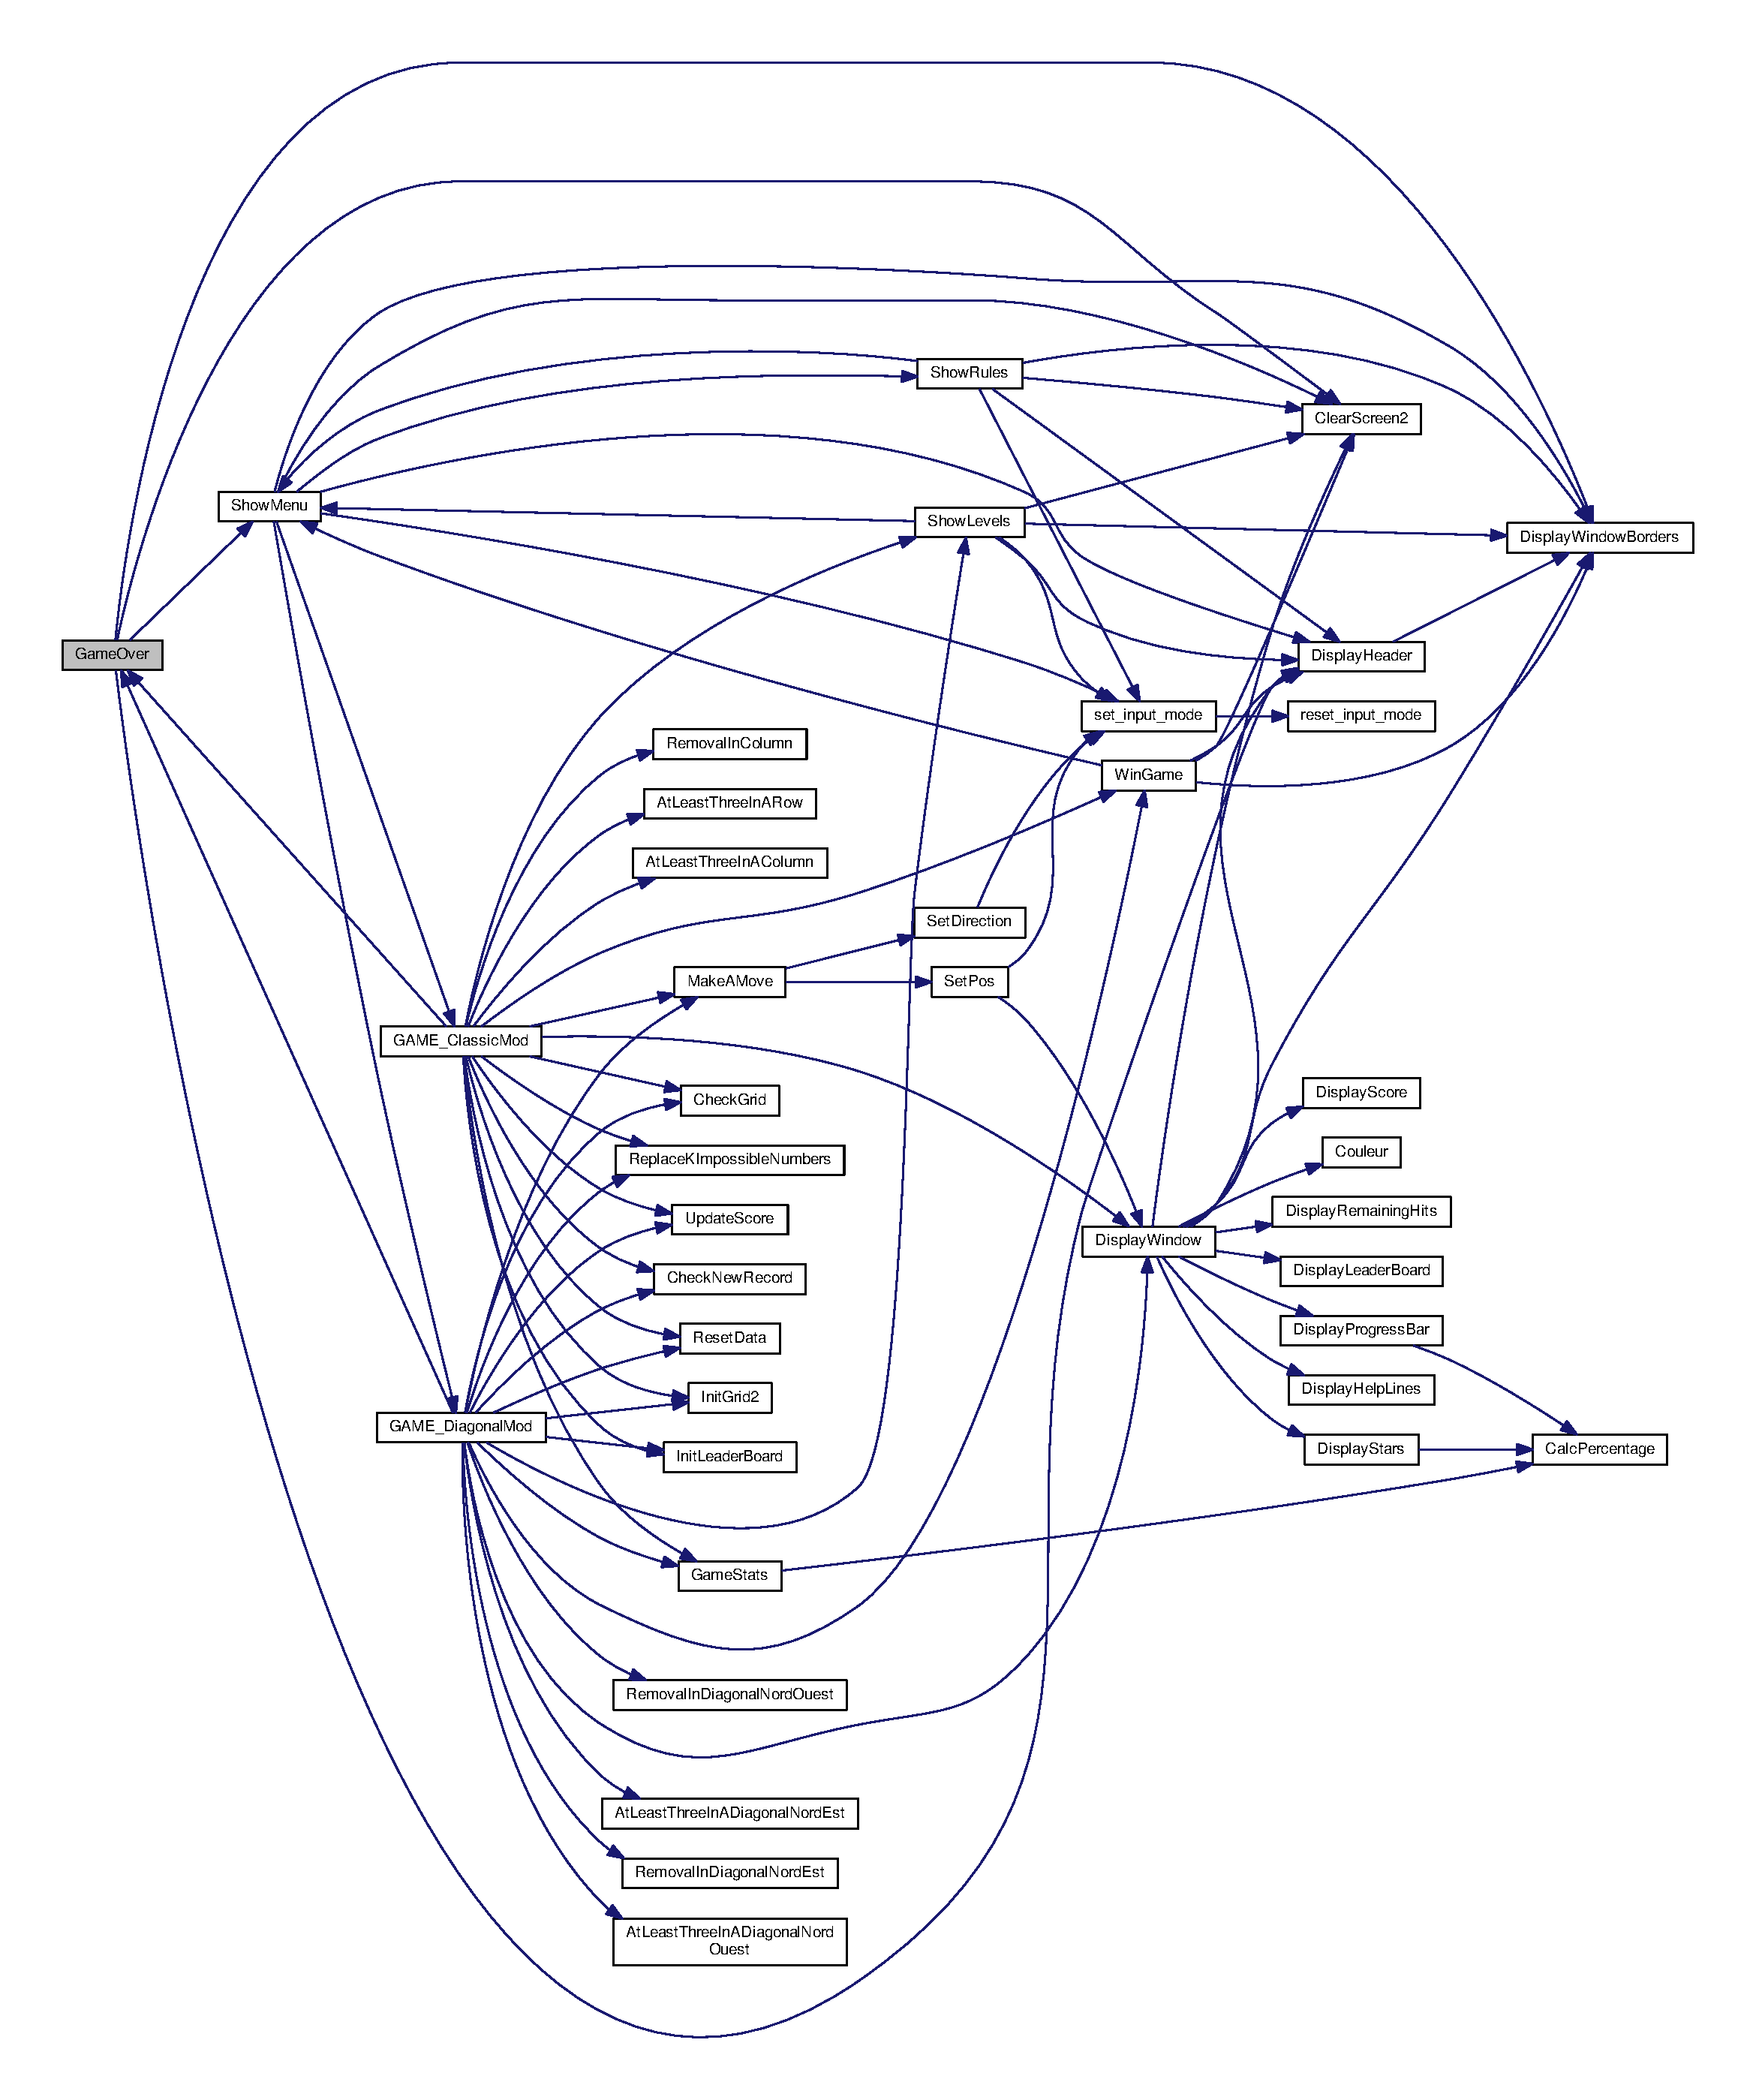
\includegraphics[width=350pt]{display_8h_ab77f0cd8eb631a2675c55cbb24bc4fee_cgraph}
\end{center}
\end{figure}




Here is the caller graph for this function\+:
\nopagebreak
\begin{figure}[H]
\begin{center}
\leavevmode
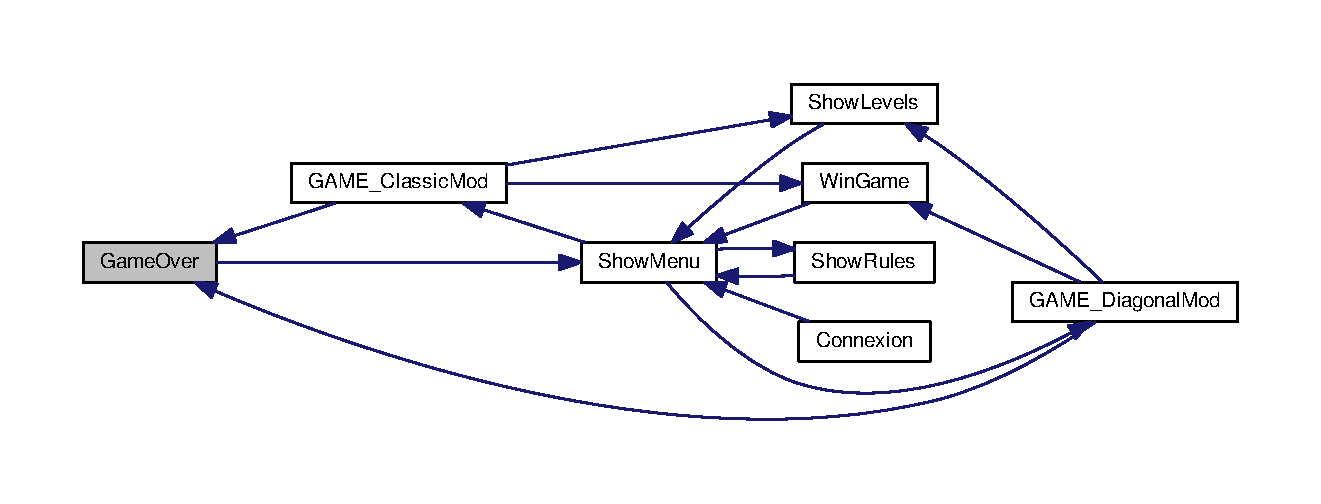
\includegraphics[width=350pt]{display_8h_ab77f0cd8eb631a2675c55cbb24bc4fee_icgraph}
\end{center}
\end{figure}


\hypertarget{display_8h_a8084e88f83b951438d2d556697b62260}{\index{display.\+h@{display.\+h}!Show\+Levels@{Show\+Levels}}
\index{Show\+Levels@{Show\+Levels}!display.\+h@{display.\+h}}
\subsubsection[{Show\+Levels}]{\setlength{\rightskip}{0pt plus 5cm}void Show\+Levels (
\begin{DoxyParamCaption}
\item[{C\+Mat \&}]{Grid, }
\item[{int \&}]{Score\+For\+Next\+Lvl, }
\item[{int \&}]{Level\+Choice, }
\item[{int \&}]{Maximal\+Hits, }
\item[{const string \&}]{Pseudo}
\end{DoxyParamCaption}
)}}\label{display_8h_a8084e88f83b951438d2d556697b62260}


Show\+Levels affiche les différents niveaux disponibles pour chaque mode de jeu. 


\begin{DoxyParams}{Parameters}
{\em Grid\mbox{[}in\mbox{]}} & Grille contenant les nombres \\
\hline
{\em Score\+For\+Next\+Lvl\mbox{[}in,out\mbox{]}} & Score à atteindre pour gagner le niveau \\
\hline
{\em Level\+Choice\mbox{[}in,out\mbox{]}} & Level choisi par l'utilisateur \\
\hline
{\em Maximal\+Hits\mbox{[}in,out\mbox{]}} & Nombre maximum de coups attribués pour le level \\
\hline
{\em Pseudo\mbox{[}in\mbox{]}} & Pseudo du joueur entré au début du jeu \\
\hline
\end{DoxyParams}


Definition at line 295 of file display.\+cpp.



Here is the call graph for this function\+:
\nopagebreak
\begin{figure}[H]
\begin{center}
\leavevmode
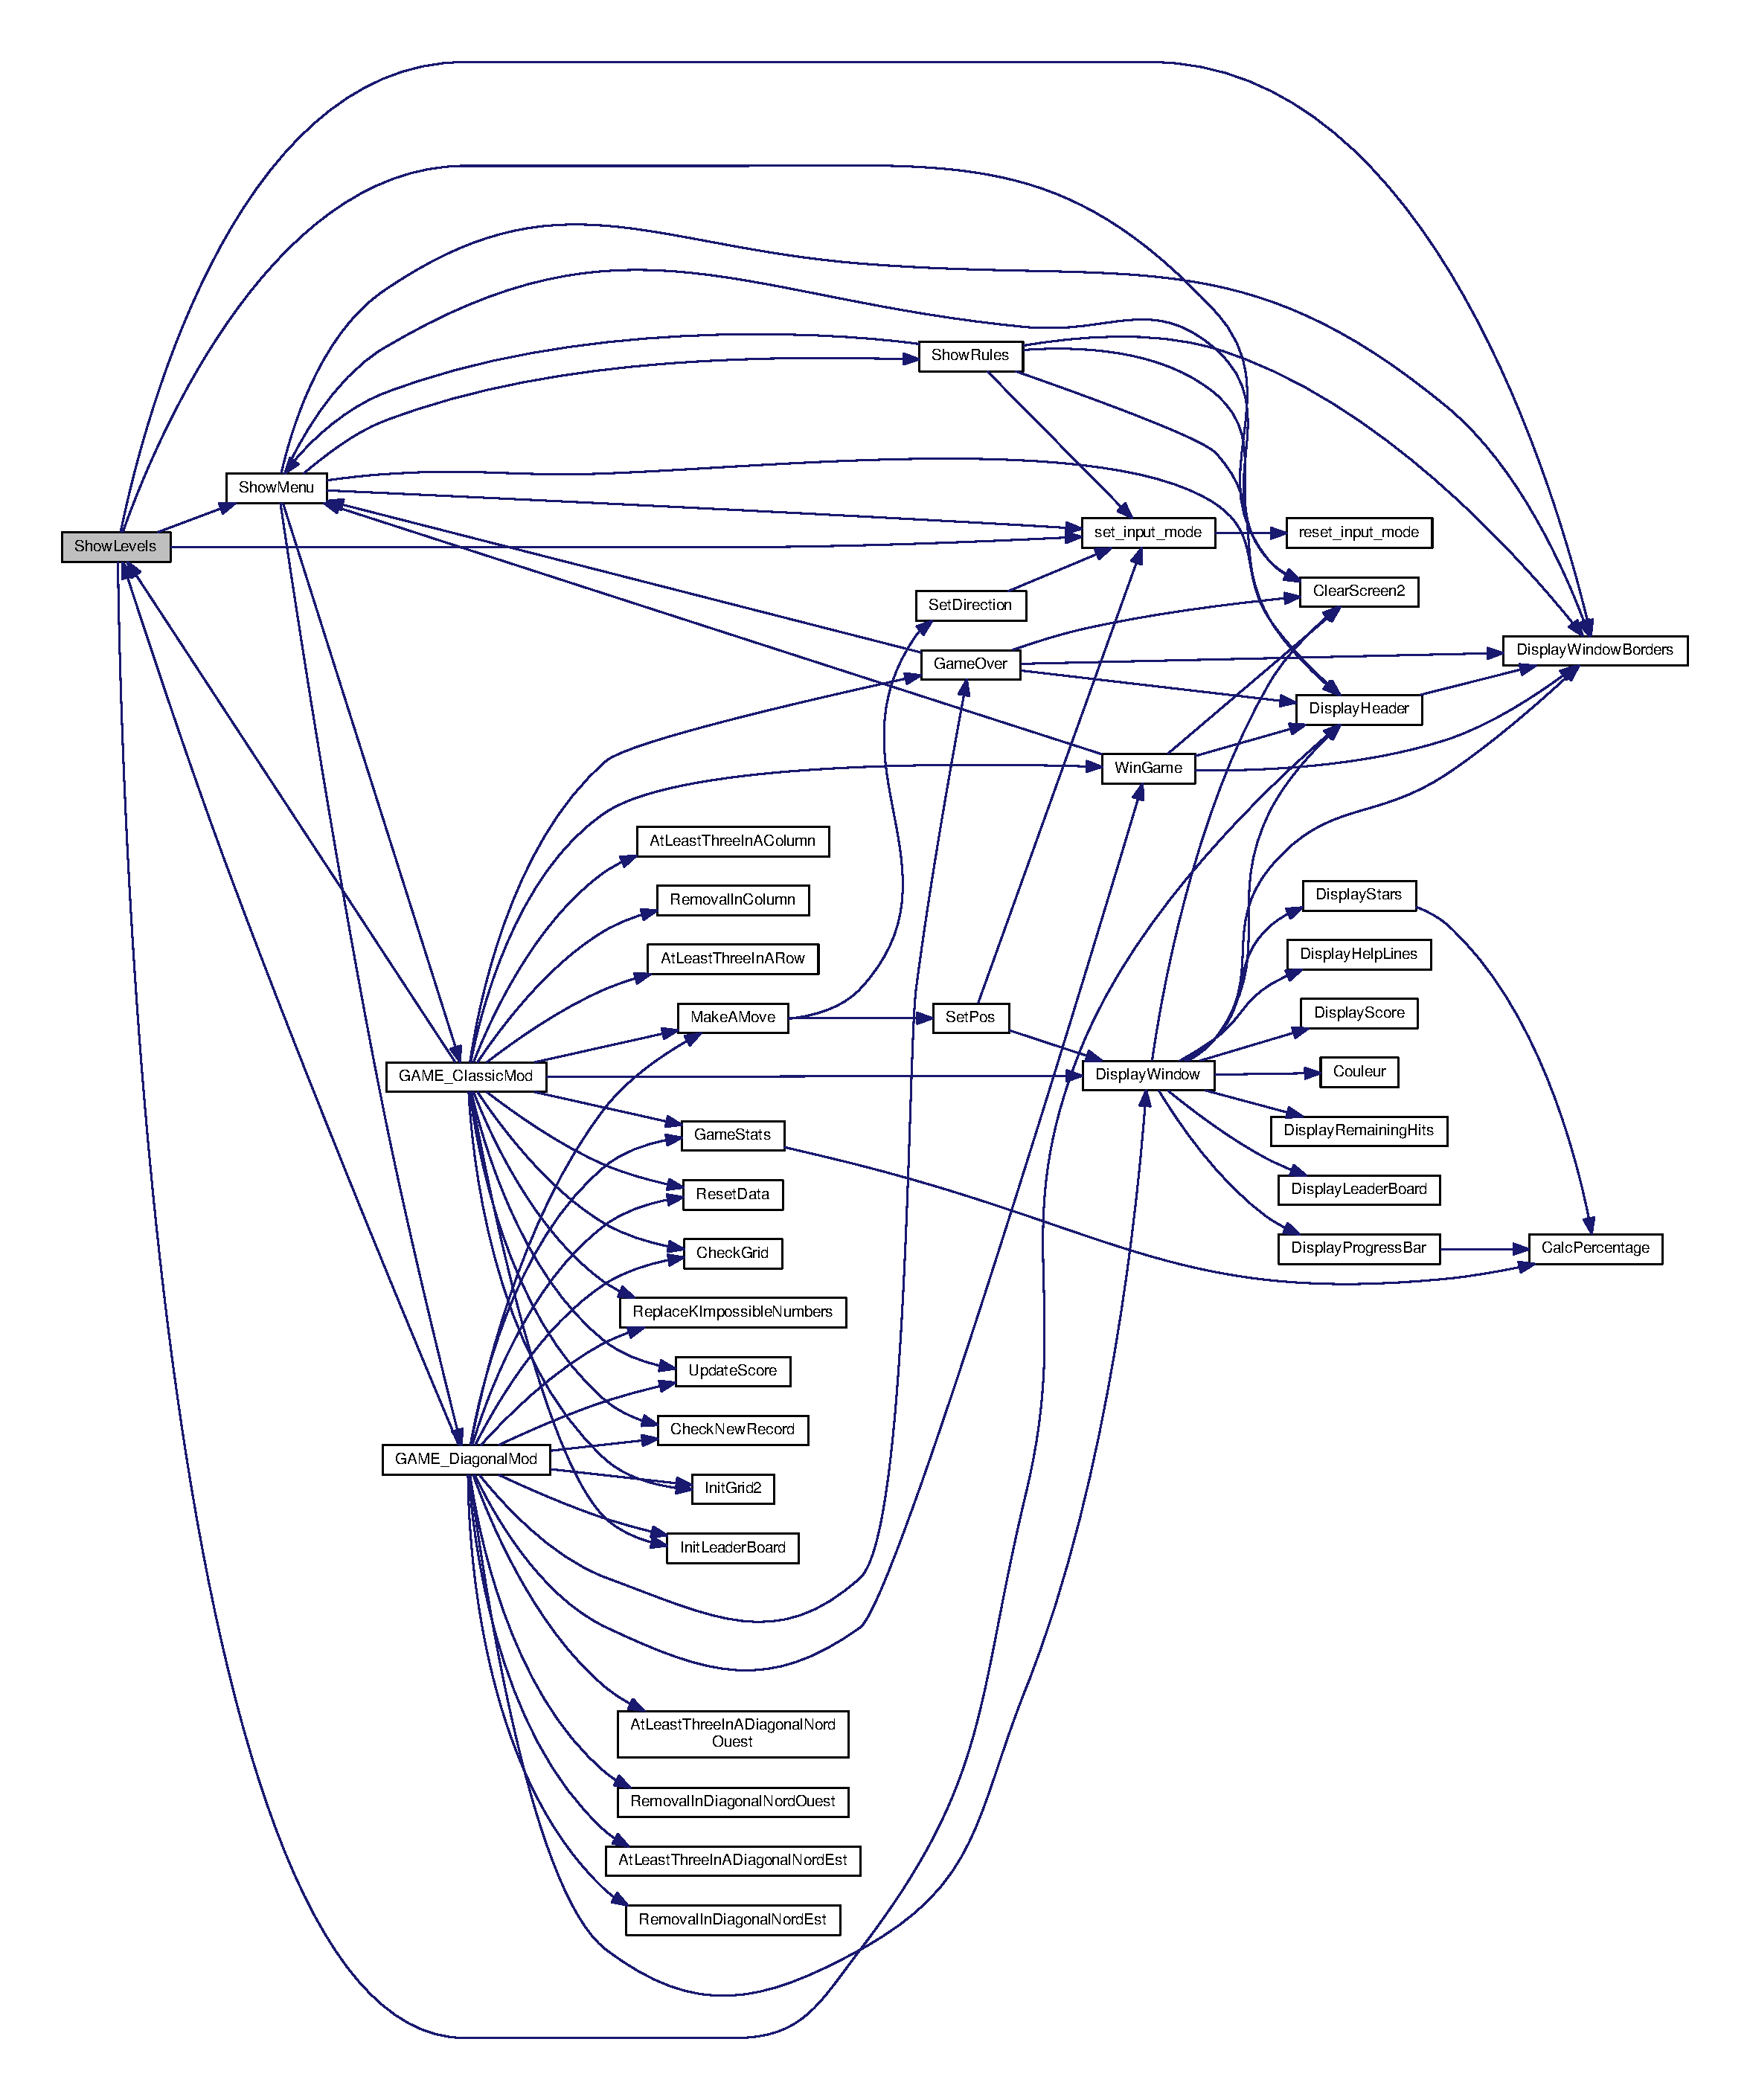
\includegraphics[width=350pt]{display_8h_a8084e88f83b951438d2d556697b62260_cgraph}
\end{center}
\end{figure}




Here is the caller graph for this function\+:
\nopagebreak
\begin{figure}[H]
\begin{center}
\leavevmode
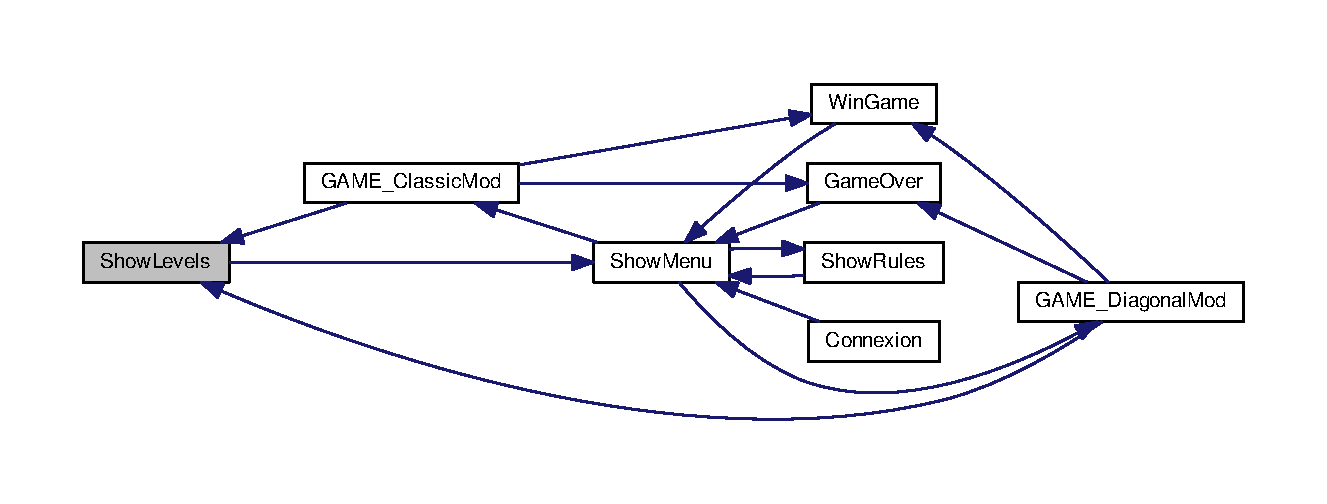
\includegraphics[width=350pt]{display_8h_a8084e88f83b951438d2d556697b62260_icgraph}
\end{center}
\end{figure}


\hypertarget{display_8h_ae89e5a96380a3c5e6d8c198020696084}{\index{display.\+h@{display.\+h}!Show\+Menu@{Show\+Menu}}
\index{Show\+Menu@{Show\+Menu}!display.\+h@{display.\+h}}
\subsubsection[{Show\+Menu}]{\setlength{\rightskip}{0pt plus 5cm}void Show\+Menu (
\begin{DoxyParamCaption}
\item[{const string \&}]{Pseudo}
\end{DoxyParamCaption}
)}}\label{display_8h_ae89e5a96380a3c5e6d8c198020696084}


Show\+Menu affiche le menu de sélection du mode de jeu (choix entre C\+L\+A\+S\+S\+I\+C, D\+I\+A\+G\+O\+N\+A\+L, R\+U\+L\+E\+S) 


\begin{DoxyParams}{Parameters}
{\em Pseudo\mbox{[}in\mbox{]}} & Pseudo du joueur entré au début du jeu \\
\hline
\end{DoxyParams}


Definition at line 224 of file display.\+cpp.



Here is the call graph for this function\+:
\nopagebreak
\begin{figure}[H]
\begin{center}
\leavevmode
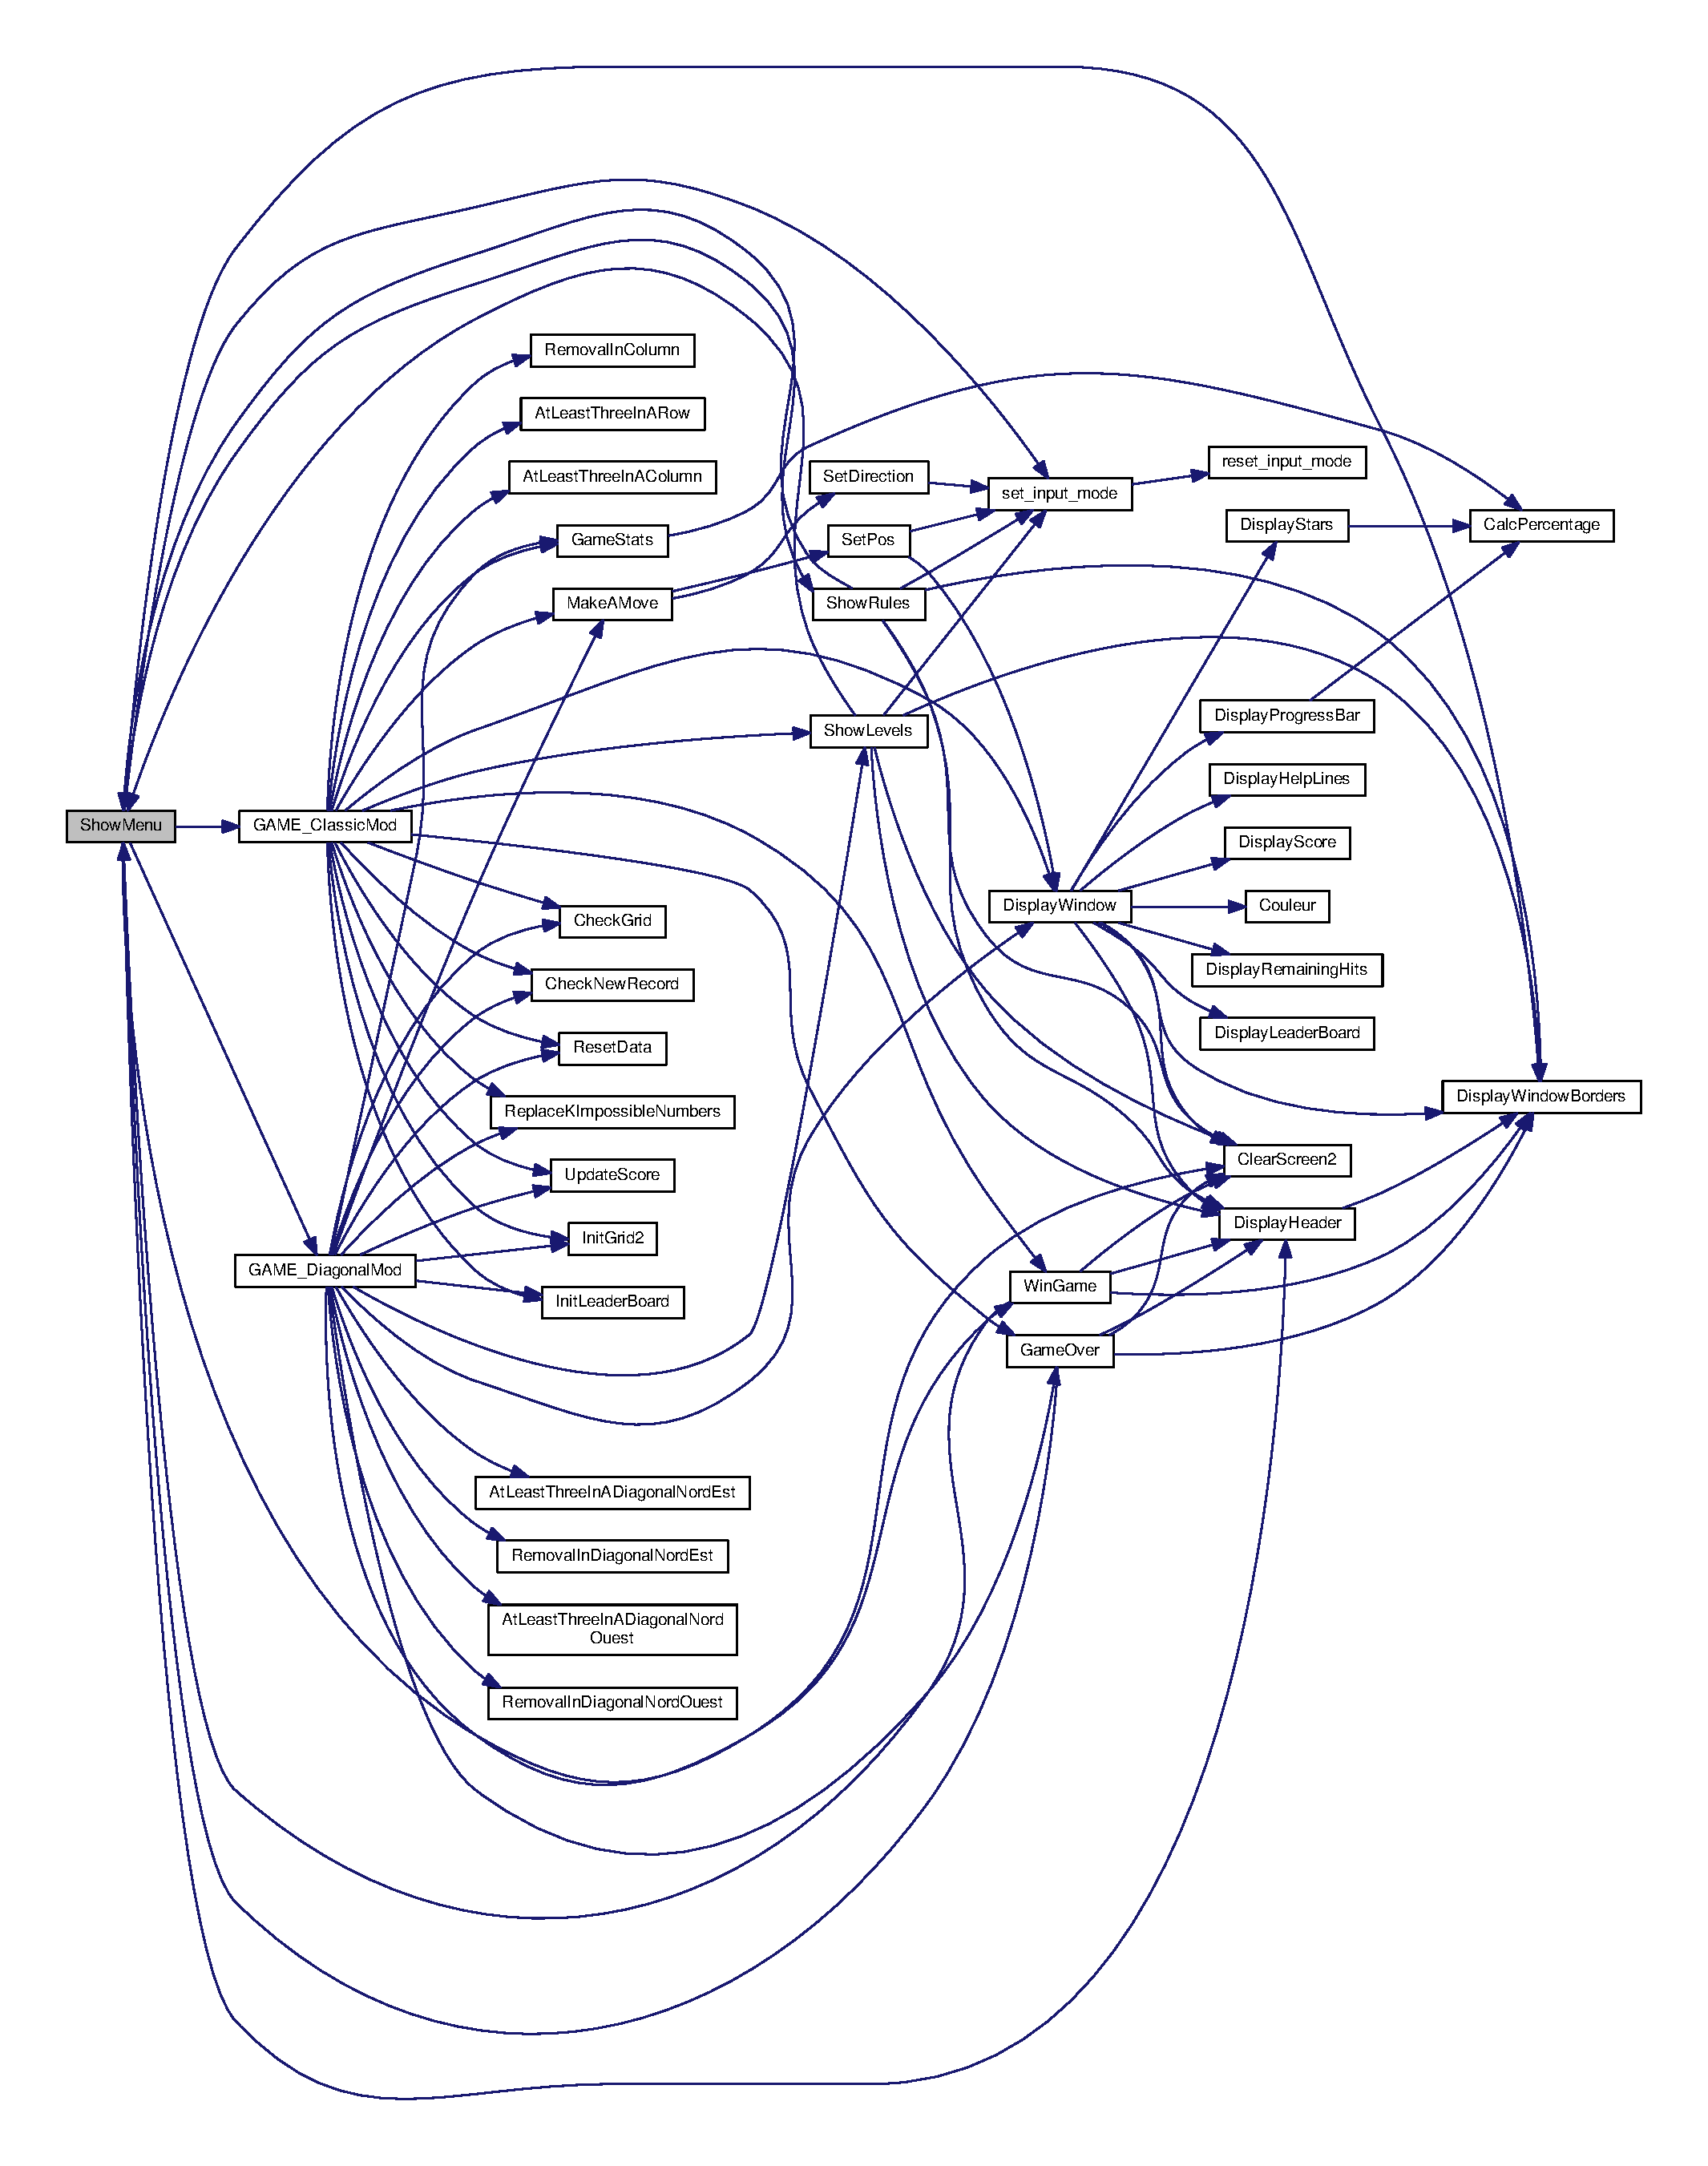
\includegraphics[width=350pt]{display_8h_ae89e5a96380a3c5e6d8c198020696084_cgraph}
\end{center}
\end{figure}




Here is the caller graph for this function\+:
\nopagebreak
\begin{figure}[H]
\begin{center}
\leavevmode
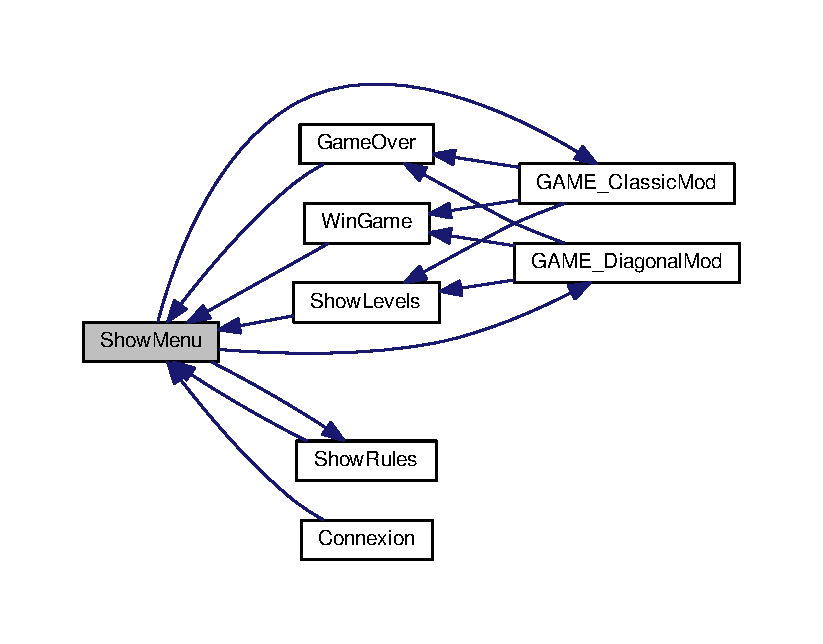
\includegraphics[width=350pt]{display_8h_ae89e5a96380a3c5e6d8c198020696084_icgraph}
\end{center}
\end{figure}


\hypertarget{display_8h_a5a4378a081a78a48ba12ec54a6a1a299}{\index{display.\+h@{display.\+h}!Show\+Rules@{Show\+Rules}}
\index{Show\+Rules@{Show\+Rules}!display.\+h@{display.\+h}}
\subsubsection[{Show\+Rules}]{\setlength{\rightskip}{0pt plus 5cm}void Show\+Rules (
\begin{DoxyParamCaption}
\item[{const string \&}]{Pseudo}
\end{DoxyParamCaption}
)}}\label{display_8h_a5a4378a081a78a48ba12ec54a6a1a299}


Show\+Rules affiche les régles des différents modes de jeu ainsi que les actions définies pour chaque touche. 


\begin{DoxyParams}{Parameters}
{\em Pseudo\mbox{[}in\mbox{]}} & Pseudo du joueur entré au début du jeu \\
\hline
\end{DoxyParams}


Definition at line 175 of file display.\+cpp.



Here is the call graph for this function\+:
\nopagebreak
\begin{figure}[H]
\begin{center}
\leavevmode
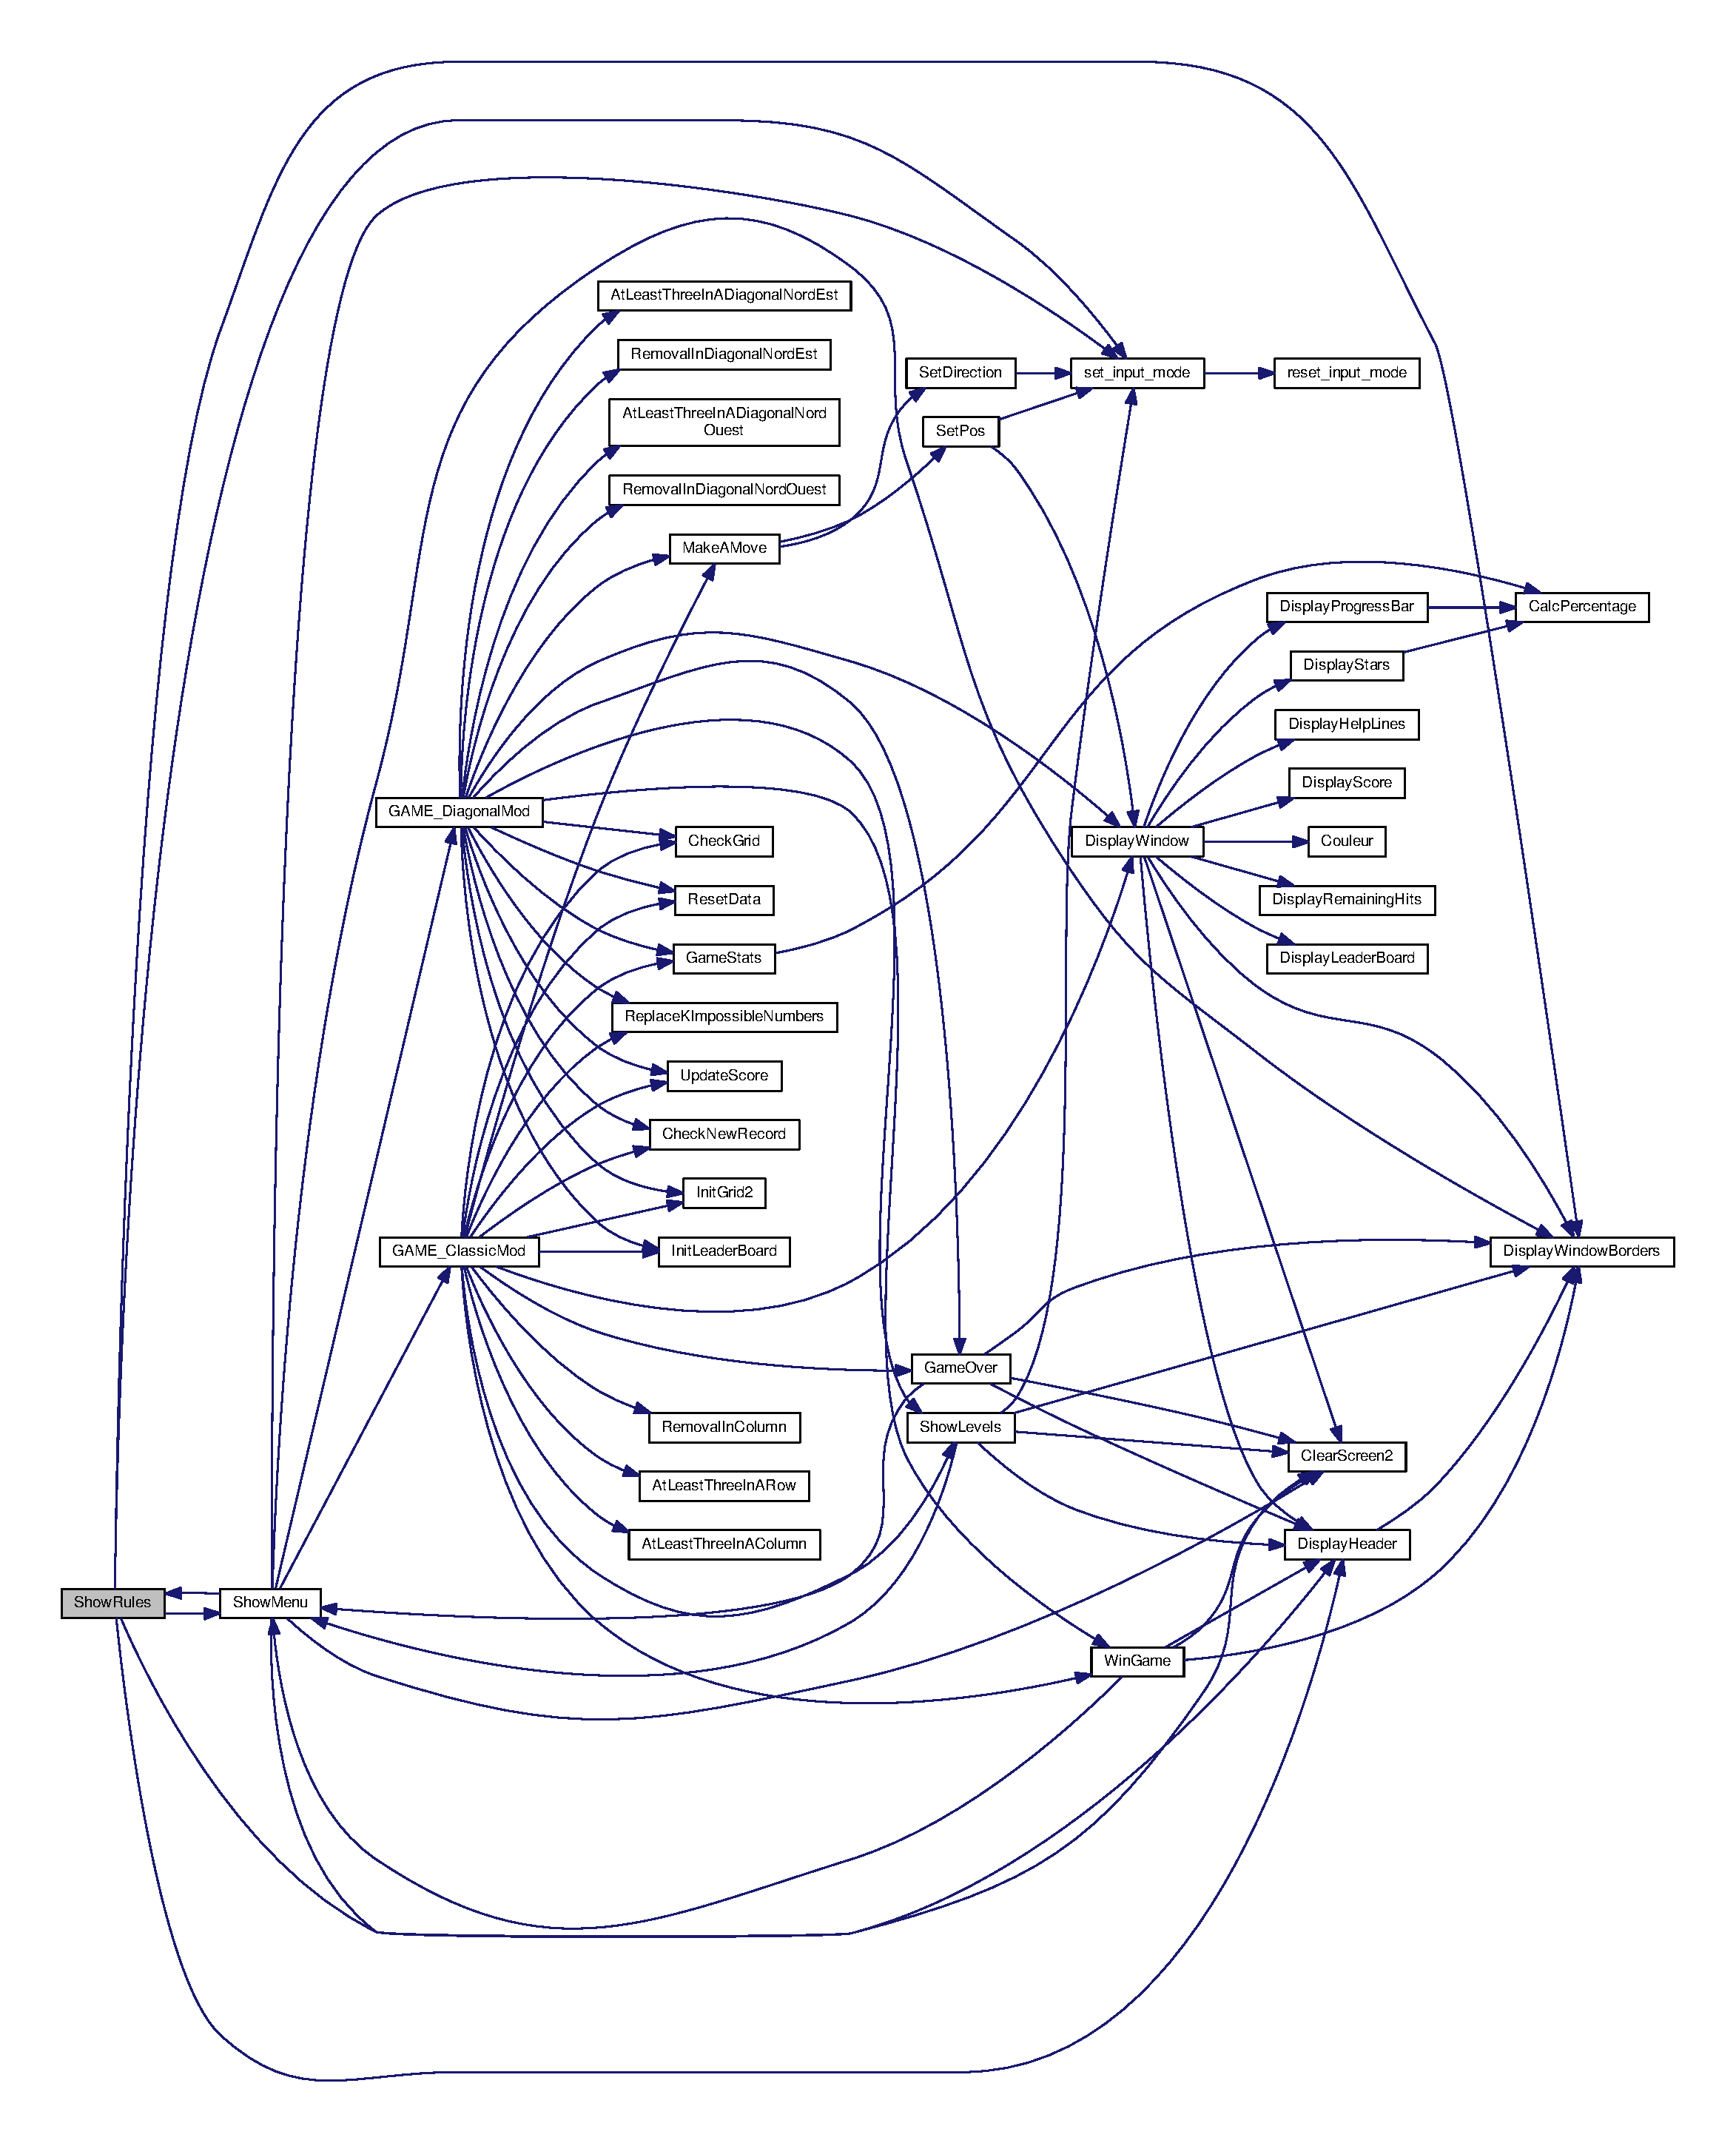
\includegraphics[width=350pt]{display_8h_a5a4378a081a78a48ba12ec54a6a1a299_cgraph}
\end{center}
\end{figure}




Here is the caller graph for this function\+:
\nopagebreak
\begin{figure}[H]
\begin{center}
\leavevmode
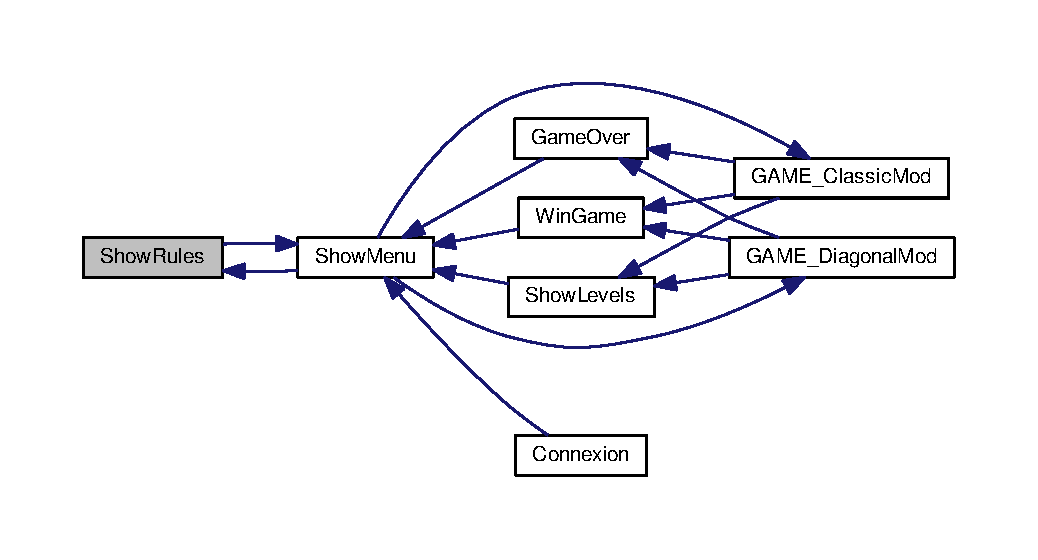
\includegraphics[width=350pt]{display_8h_a5a4378a081a78a48ba12ec54a6a1a299_icgraph}
\end{center}
\end{figure}


\hypertarget{display_8h_a2136d186fc0e7a3e00be122068e5810c}{\index{display.\+h@{display.\+h}!Win\+Game@{Win\+Game}}
\index{Win\+Game@{Win\+Game}!display.\+h@{display.\+h}}
\subsubsection[{Win\+Game}]{\setlength{\rightskip}{0pt plus 5cm}void Win\+Game (
\begin{DoxyParamCaption}
\item[{const string \&}]{Pseudo}
\end{DoxyParamCaption}
)}}\label{display_8h_a2136d186fc0e7a3e00be122068e5810c}


Win\+Game affiche la fenêtre \char`\"{}\+Y\+O\+U W\+I\+N\char`\"{} lorsque le joueur a gagné 


\begin{DoxyParams}{Parameters}
{\em Pseudo\mbox{[}in\mbox{]}} & Pseudo du joueur entré au début du jeu \\
\hline
\end{DoxyParams}


Definition at line 159 of file display.\+cpp.



Here is the call graph for this function\+:
\nopagebreak
\begin{figure}[H]
\begin{center}
\leavevmode
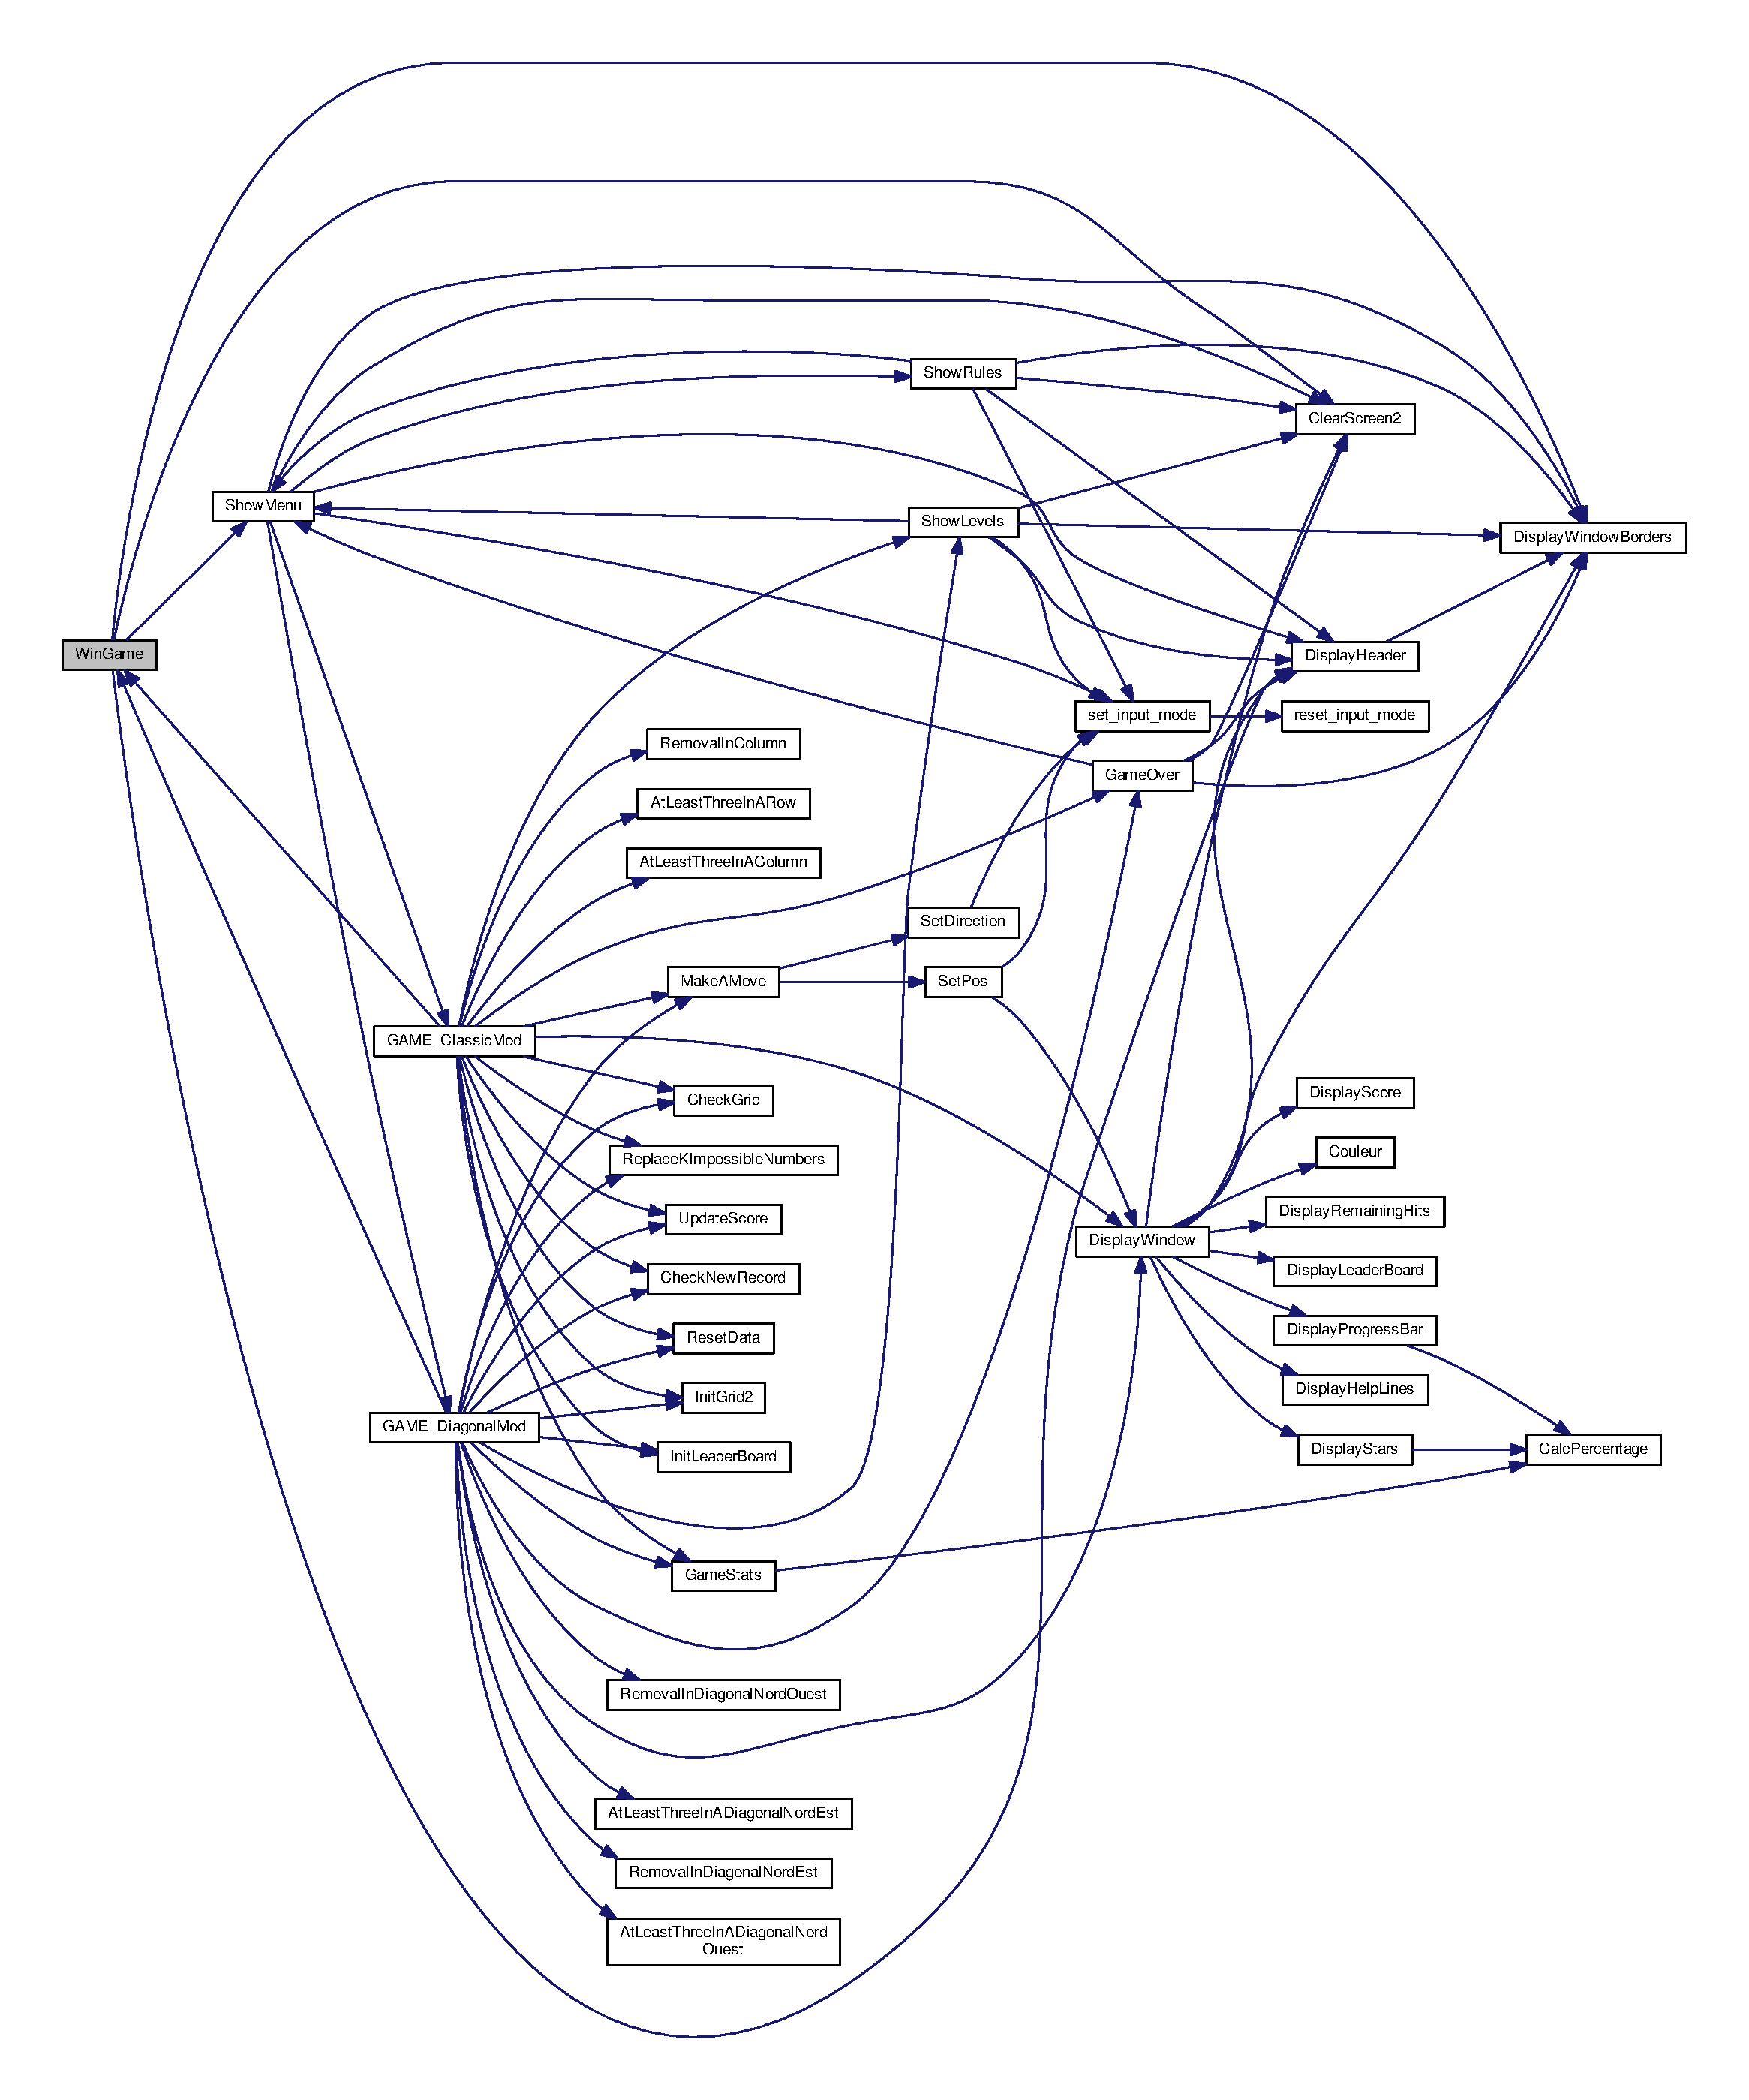
\includegraphics[width=350pt]{display_8h_a2136d186fc0e7a3e00be122068e5810c_cgraph}
\end{center}
\end{figure}




Here is the caller graph for this function\+:
\nopagebreak
\begin{figure}[H]
\begin{center}
\leavevmode
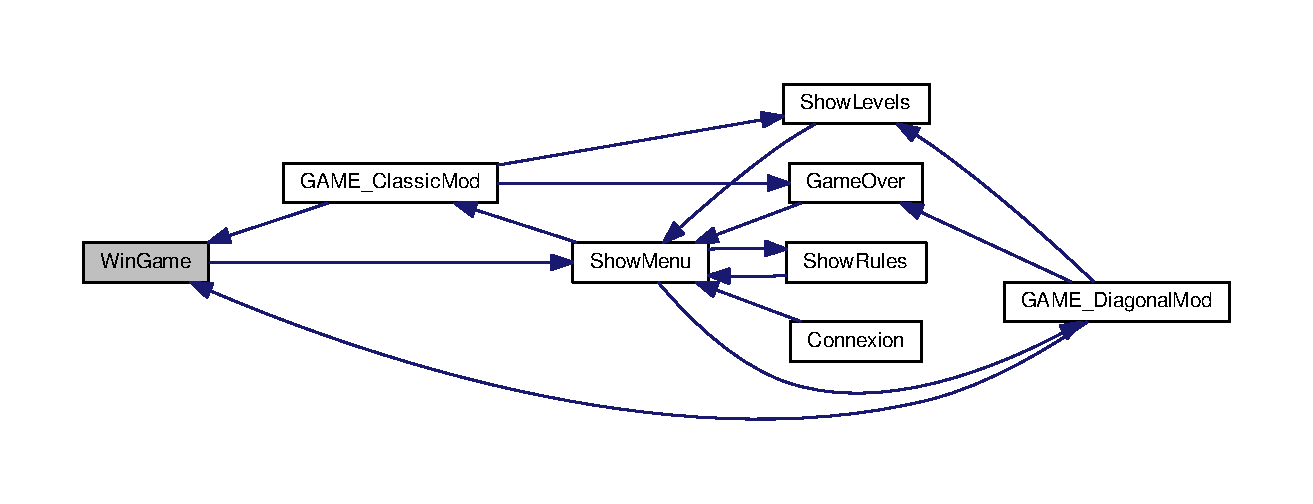
\includegraphics[width=350pt]{display_8h_a2136d186fc0e7a3e00be122068e5810c_icgraph}
\end{center}
\end{figure}



\hypertarget{gamemods_8h}{\section{gamemods.\+h File Reference}
\label{gamemods_8h}\index{gamemods.\+h@{gamemods.\+h}}
}


Les différents modes de jeu.  


{\ttfamily \#include \char`\"{}params2.\+h\char`\"{}}\\*
Include dependency graph for gamemods.\+h\+:
\nopagebreak
\begin{figure}[H]
\begin{center}
\leavevmode
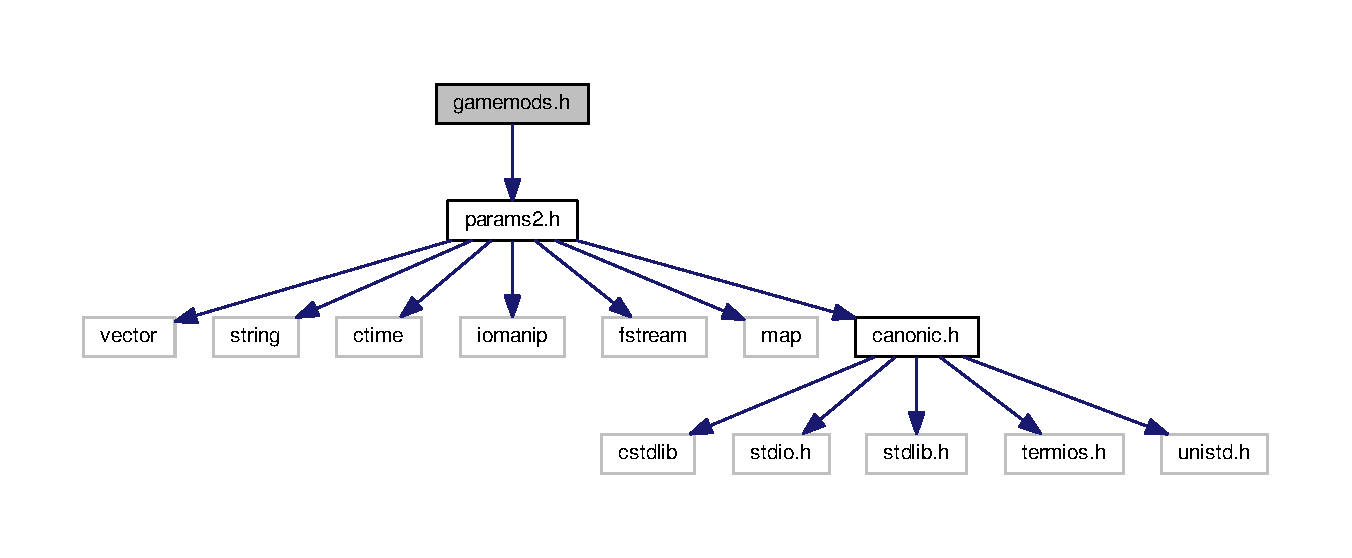
\includegraphics[width=350pt]{gamemods_8h__incl}
\end{center}
\end{figure}
This graph shows which files directly or indirectly include this file\+:
\nopagebreak
\begin{figure}[H]
\begin{center}
\leavevmode
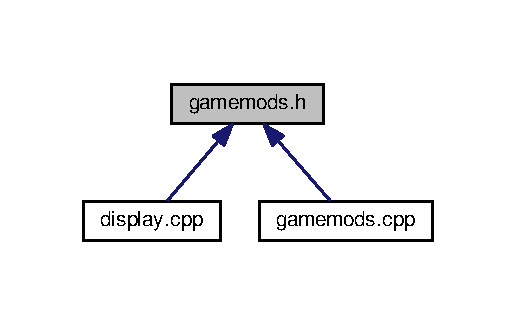
\includegraphics[width=248pt]{gamemods_8h__dep__incl}
\end{center}
\end{figure}
\subsection*{Functions}
\begin{DoxyCompactItemize}
\item 
void \hyperlink{gamemods_8h_a4735fa2a3f1f10abe10b610510680b3c}{G\+A\+M\+E\+\_\+\+Classic\+Mod} (int \&Game\+Choice, const string \&Pseudo)
\begin{DoxyCompactList}\small\item\em G\+A\+M\+E\+\_\+\+Classic\+Mod permet de jouer en mode classique du jeu c'est-\/à-\/dire qu'il faut aligner au moins 3 chiffres en ligne ou en colonne. \end{DoxyCompactList}\item 
void \hyperlink{gamemods_8h_afb4190e75f694b88fc919cb938bb9d6d}{G\+A\+M\+E\+\_\+\+Diagonal\+Mod} (int \&Game\+Choice, const string \&Pseudo)
\begin{DoxyCompactList}\small\item\em G\+A\+M\+E\+\_\+\+Diagonal\+Mod permet de jouer en mode diagonal du jeu c'est-\/à-\/dire qu'il faut aligner au moins 3 chiffres en diagonale. \end{DoxyCompactList}\end{DoxyCompactItemize}


\subsection{Detailed Description}
Les différents modes de jeu. 

\begin{DoxyAuthor}{Author}
Quentin Pla, Léo Vincent, Emma tarfi, Sirine Achache, Julien Vavrille
\end{DoxyAuthor}
\begin{DoxyDate}{Date}
26 janvier 2018 
\end{DoxyDate}


Definition in file \hyperlink{gamemods_8h_source}{gamemods.\+h}.



\subsection{Function Documentation}
\hypertarget{gamemods_8h_a4735fa2a3f1f10abe10b610510680b3c}{\index{gamemods.\+h@{gamemods.\+h}!G\+A\+M\+E\+\_\+\+Classic\+Mod@{G\+A\+M\+E\+\_\+\+Classic\+Mod}}
\index{G\+A\+M\+E\+\_\+\+Classic\+Mod@{G\+A\+M\+E\+\_\+\+Classic\+Mod}!gamemods.\+h@{gamemods.\+h}}
\subsubsection[{G\+A\+M\+E\+\_\+\+Classic\+Mod}]{\setlength{\rightskip}{0pt plus 5cm}void G\+A\+M\+E\+\_\+\+Classic\+Mod (
\begin{DoxyParamCaption}
\item[{int \&}]{Game\+Choice, }
\item[{const string \&}]{Pseudo}
\end{DoxyParamCaption}
)}}\label{gamemods_8h_a4735fa2a3f1f10abe10b610510680b3c}


G\+A\+M\+E\+\_\+\+Classic\+Mod permet de jouer en mode classique du jeu c'est-\/à-\/dire qu'il faut aligner au moins 3 chiffres en ligne ou en colonne. 


\begin{DoxyParams}{Parameters}
{\em Game\+Choice\mbox{[}in\mbox{]}} & le mode de jeu que l'on a choisi \\
\hline
{\em Pseudo\mbox{[}in\mbox{]}} & le pseudo que l'on a rentré \\
\hline
\end{DoxyParams}


Definition at line 10 of file gamemods.\+cpp.



Here is the call graph for this function\+:
\nopagebreak
\begin{figure}[H]
\begin{center}
\leavevmode
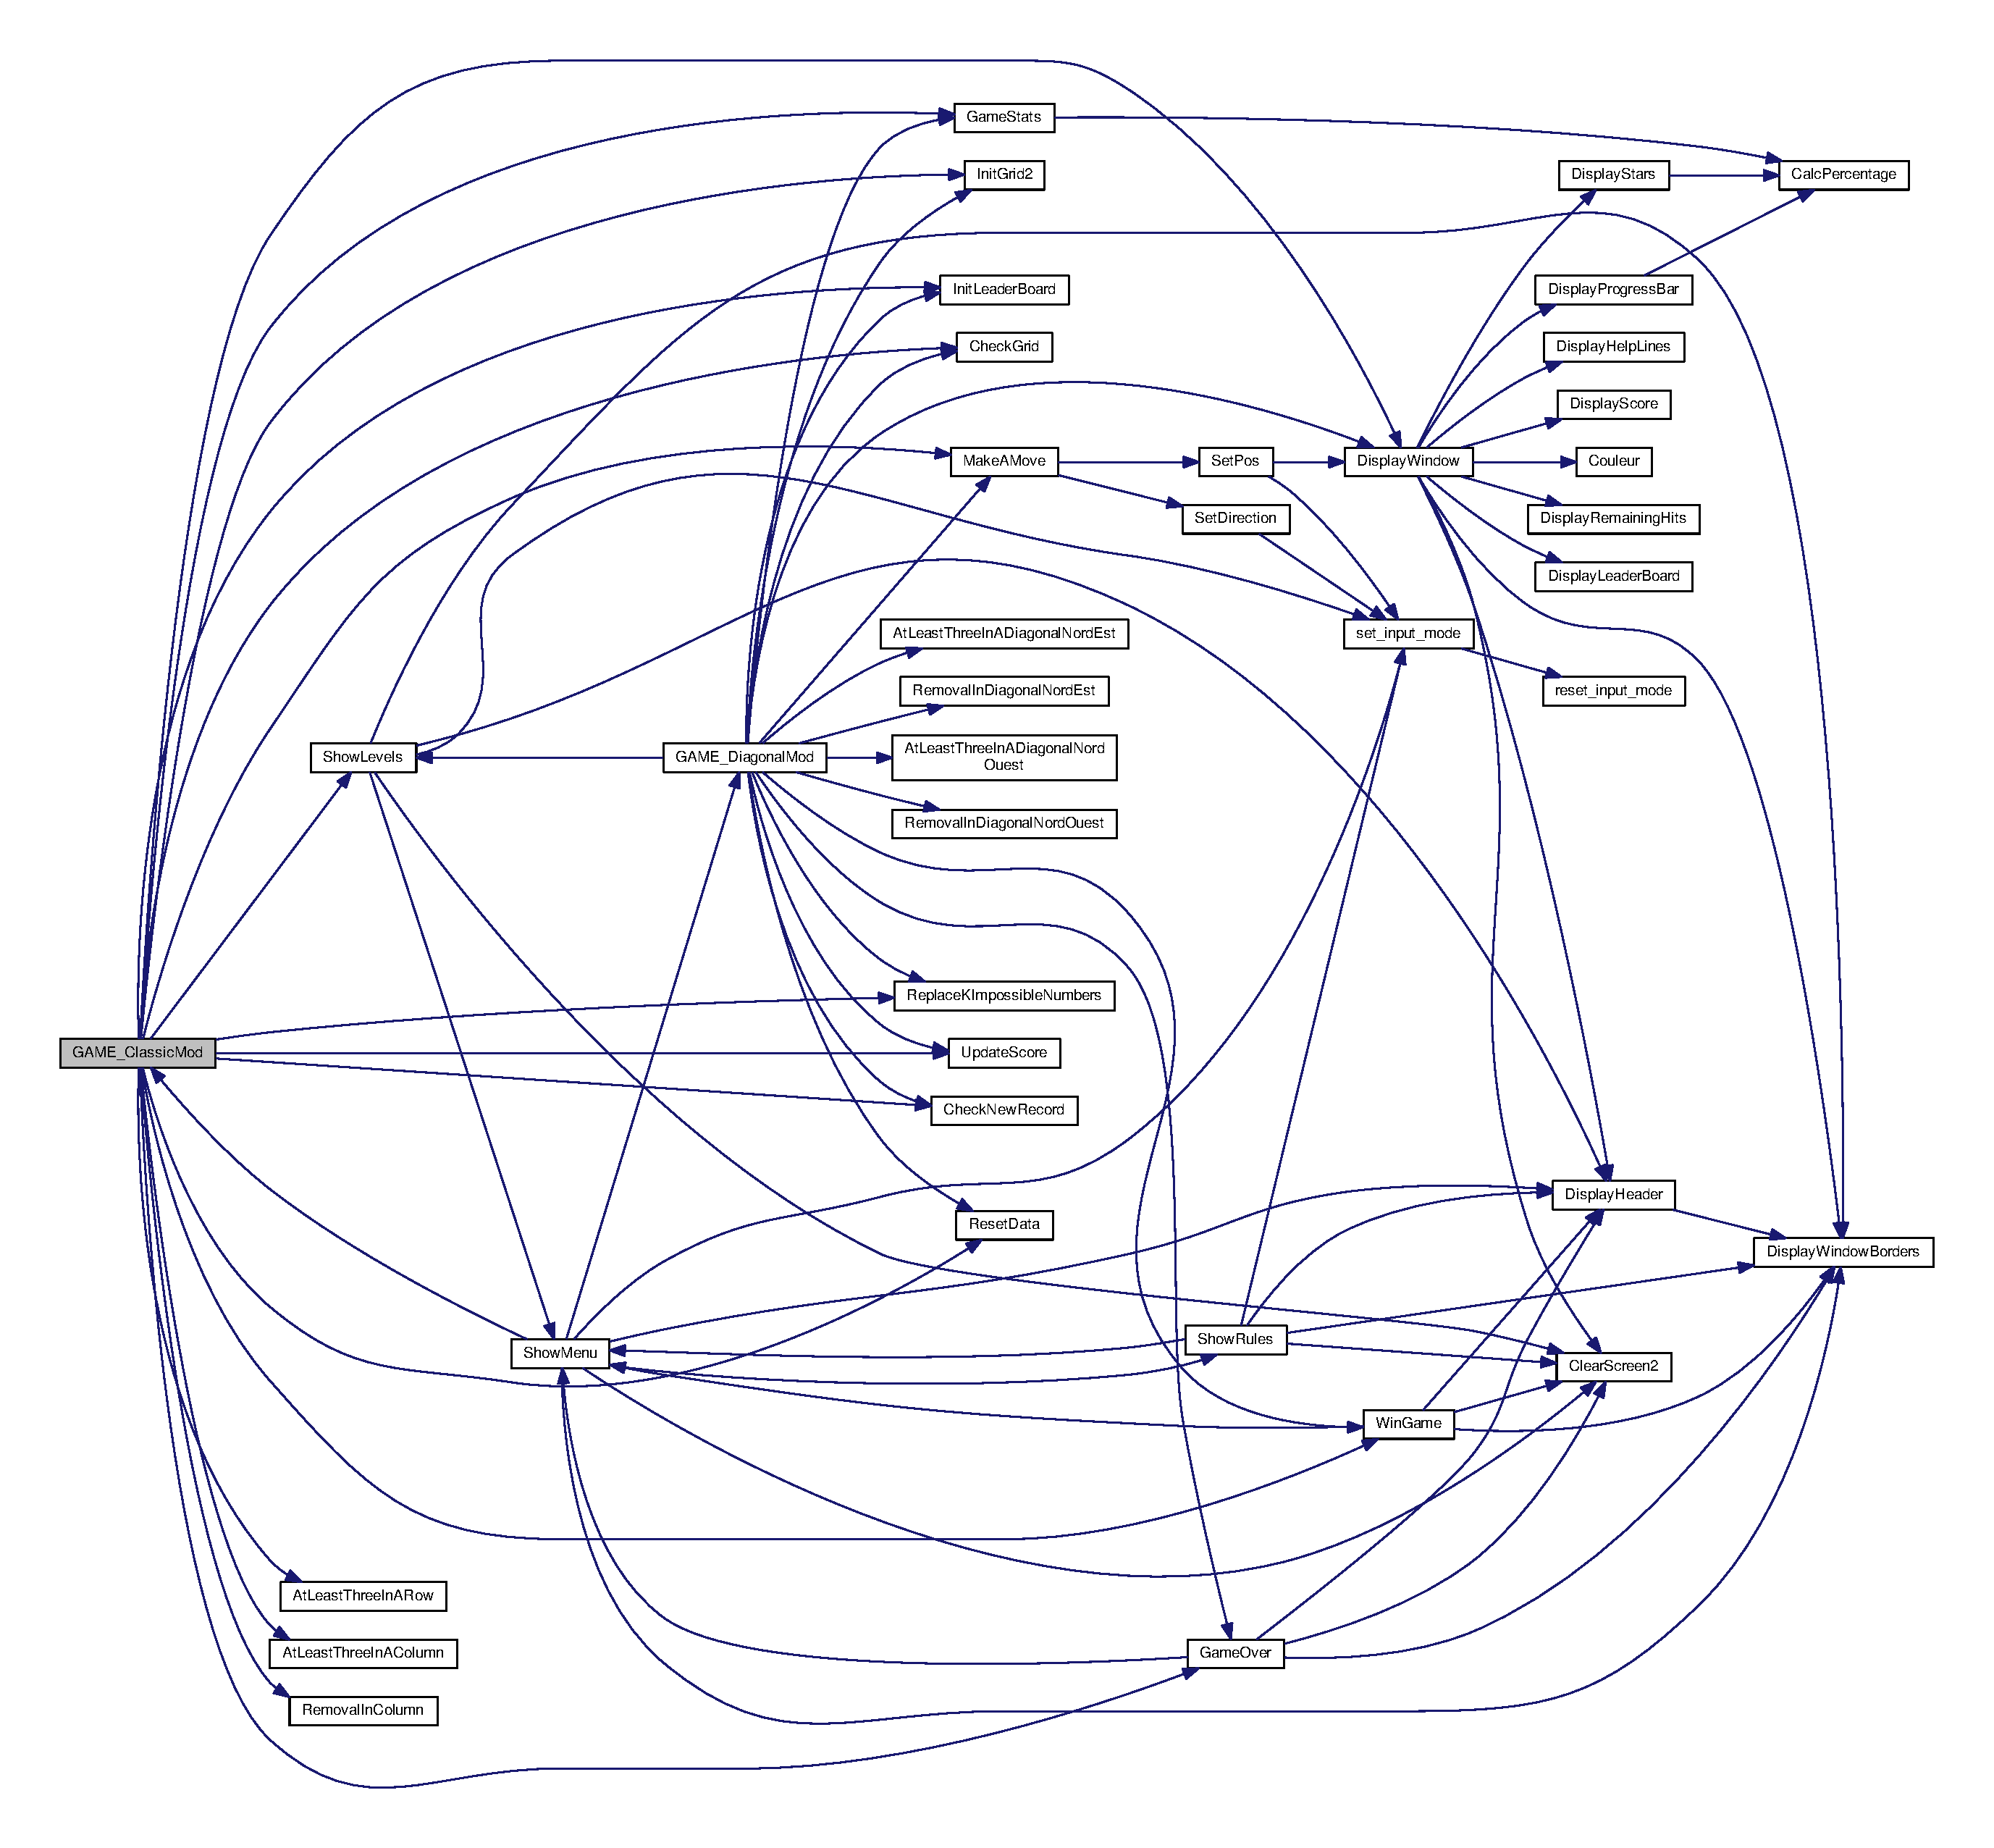
\includegraphics[width=350pt]{gamemods_8h_a4735fa2a3f1f10abe10b610510680b3c_cgraph}
\end{center}
\end{figure}




Here is the caller graph for this function\+:
\nopagebreak
\begin{figure}[H]
\begin{center}
\leavevmode
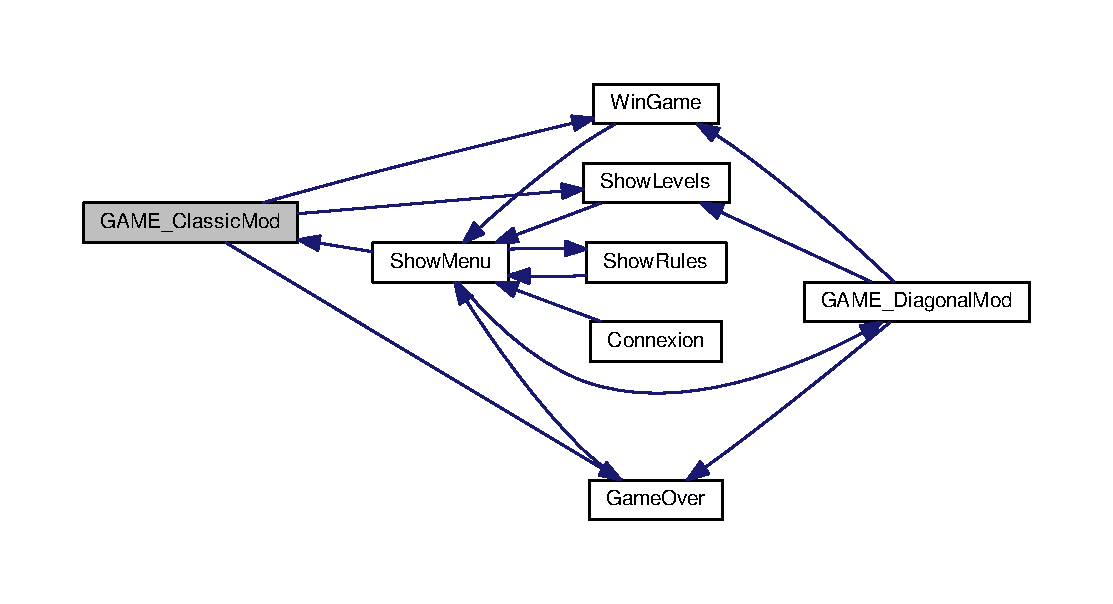
\includegraphics[width=350pt]{gamemods_8h_a4735fa2a3f1f10abe10b610510680b3c_icgraph}
\end{center}
\end{figure}


\hypertarget{gamemods_8h_afb4190e75f694b88fc919cb938bb9d6d}{\index{gamemods.\+h@{gamemods.\+h}!G\+A\+M\+E\+\_\+\+Diagonal\+Mod@{G\+A\+M\+E\+\_\+\+Diagonal\+Mod}}
\index{G\+A\+M\+E\+\_\+\+Diagonal\+Mod@{G\+A\+M\+E\+\_\+\+Diagonal\+Mod}!gamemods.\+h@{gamemods.\+h}}
\subsubsection[{G\+A\+M\+E\+\_\+\+Diagonal\+Mod}]{\setlength{\rightskip}{0pt plus 5cm}void G\+A\+M\+E\+\_\+\+Diagonal\+Mod (
\begin{DoxyParamCaption}
\item[{int \&}]{Game\+Choice, }
\item[{const string \&}]{Pseudo}
\end{DoxyParamCaption}
)}}\label{gamemods_8h_afb4190e75f694b88fc919cb938bb9d6d}


G\+A\+M\+E\+\_\+\+Diagonal\+Mod permet de jouer en mode diagonal du jeu c'est-\/à-\/dire qu'il faut aligner au moins 3 chiffres en diagonale. 


\begin{DoxyParams}{Parameters}
{\em Game\+Choice\mbox{[}in\mbox{]}} & le mode de jeu que l'on a choisi \\
\hline
{\em Pseudo\mbox{[}in\mbox{]}} & le pseudo que l'on a rentré \\
\hline
\end{DoxyParams}


Definition at line 73 of file gamemods.\+cpp.



Here is the call graph for this function\+:
\nopagebreak
\begin{figure}[H]
\begin{center}
\leavevmode
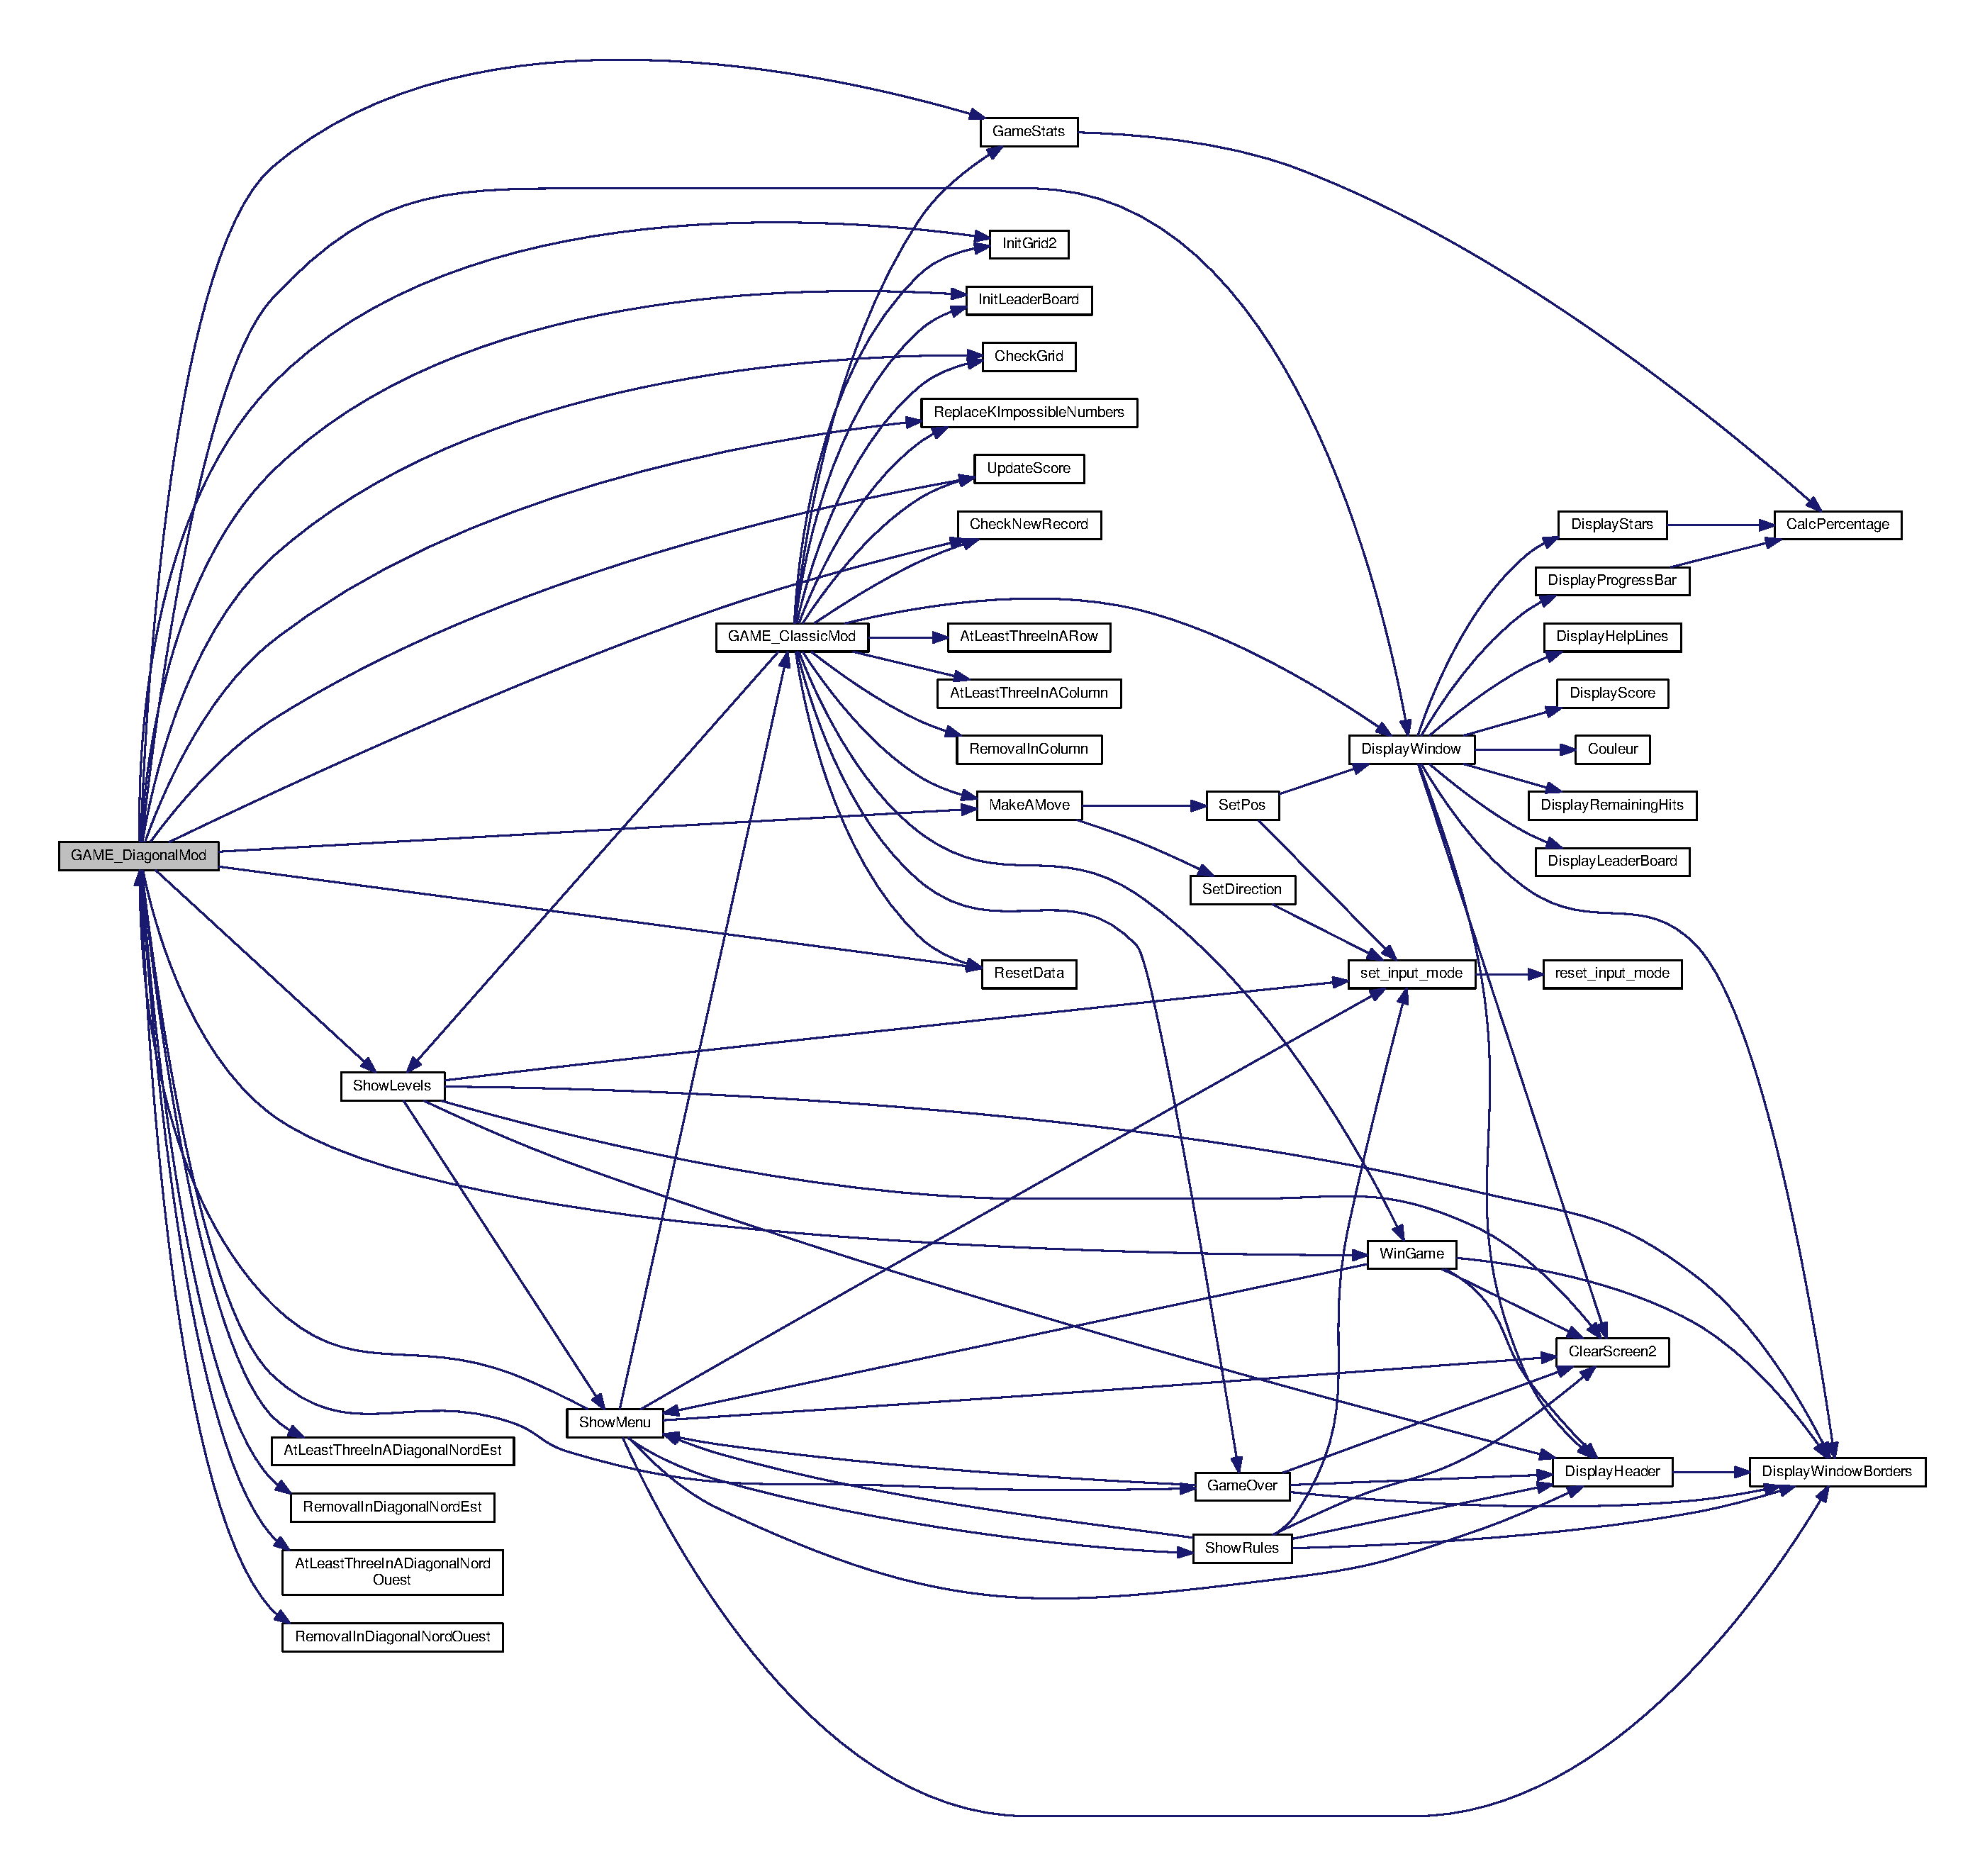
\includegraphics[width=350pt]{gamemods_8h_afb4190e75f694b88fc919cb938bb9d6d_cgraph}
\end{center}
\end{figure}




Here is the caller graph for this function\+:
\nopagebreak
\begin{figure}[H]
\begin{center}
\leavevmode
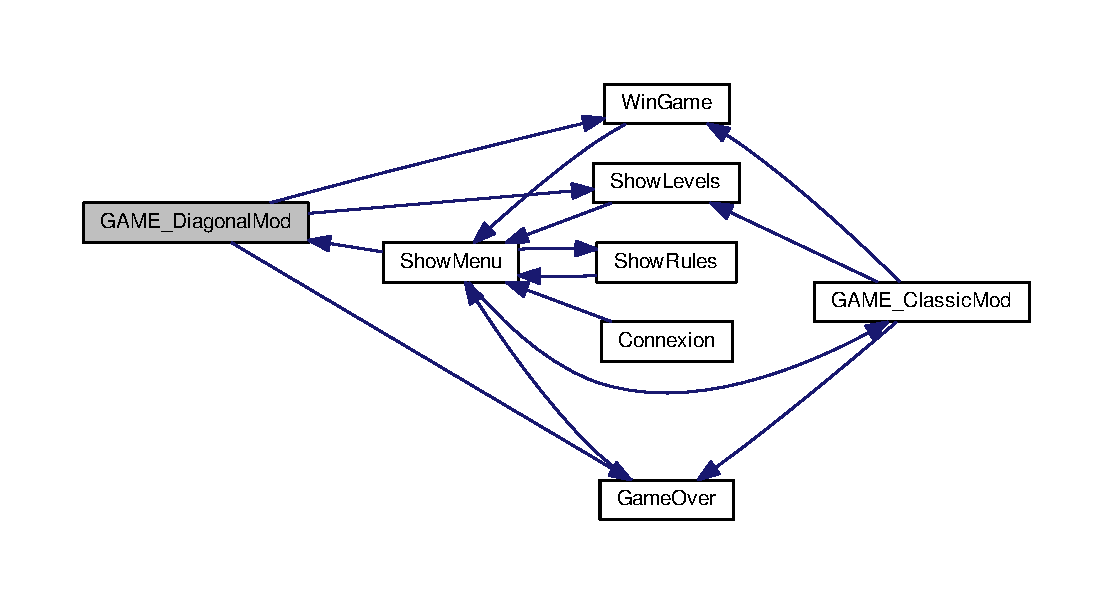
\includegraphics[width=350pt]{gamemods_8h_afb4190e75f694b88fc919cb938bb9d6d_icgraph}
\end{center}
\end{figure}



\hypertarget{ingame_8h}{\section{ingame.\+h File Reference}
\label{ingame_8h}\index{ingame.\+h@{ingame.\+h}}
}


Fonctionnalité du jeu en interaction avec le joueur.  


{\ttfamily \#include \char`\"{}params2.\+h\char`\"{}}\\*
Include dependency graph for ingame.\+h\+:
\nopagebreak
\begin{figure}[H]
\begin{center}
\leavevmode
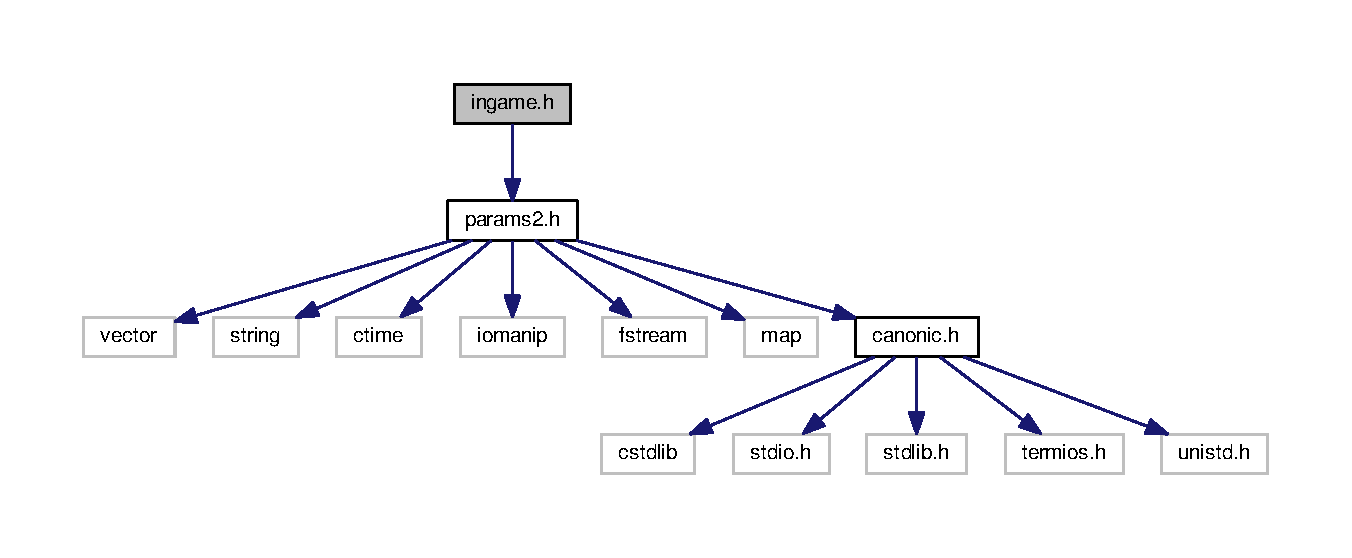
\includegraphics[width=350pt]{ingame_8h__incl}
\end{center}
\end{figure}
This graph shows which files directly or indirectly include this file\+:
\nopagebreak
\begin{figure}[H]
\begin{center}
\leavevmode
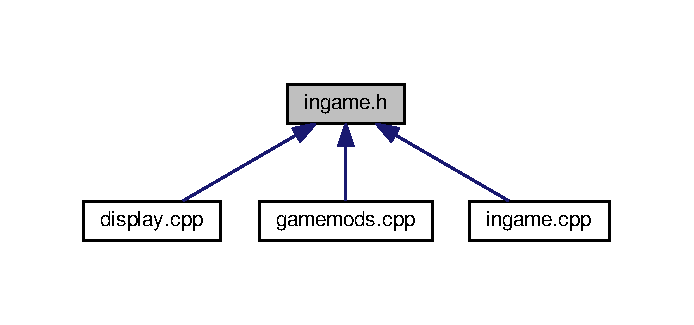
\includegraphics[width=333pt]{ingame_8h__dep__incl}
\end{center}
\end{figure}
\subsection*{Functions}
\begin{DoxyCompactItemize}
\item 
void \hyperlink{ingame_8h_afbd1bef0eeee45e421b3578f66acba35}{Set\+Pos} (C\+Position \&Pos, const C\+Mat \&Grid, const C\+Mat\+Str \&Leader\+Board, int \&Score\+For\+Next\+Lvl, int \&Score, int \&Level\+Choice, int \&Maximal\+Hits, int \&Hits)
\begin{DoxyCompactList}\small\item\em Set\+Pos permet de sélectionner la position horizontale et verticale de la case que l'on souhaite. \end{DoxyCompactList}\item 
void \hyperlink{ingame_8h_a295fed03353e3a7d18d3a64a572b99ec}{Set\+Direction} (C\+Mat \&Grid, C\+Position \&Pos, char \&Direction, bool \&Next\+Number)
\begin{DoxyCompactList}\small\item\em Set\+Direction permet de choisir la directionn souhaitée (haut, bas , gauche, droite) \end{DoxyCompactList}\item 
void \hyperlink{ingame_8h_a60837ded3ac39240259c93509f783ba8}{Make\+A\+Move} (C\+Mat \&Grid, C\+Position \&Pos, char \&Direction, bool \&Next\+Number, const C\+Mat\+Str \&Leader\+Board, int \&Score\+For\+Next\+Lvl, int \&Score, int \&Level\+Choice, int \&Maximal\+Hits, int \&Hits)
\begin{DoxyCompactList}\small\item\em Make\+A\+Move. \end{DoxyCompactList}\item 
void \hyperlink{ingame_8h_a3782b9c91c01c218dd60721fa091a274}{Removal\+In\+Diagonal\+Nord\+Est} (C\+Mat \&Grid, const C\+Position \&Pos, unsigned \&How\+Many)
\begin{DoxyCompactList}\small\item\em Removal\+In\+Diagonal\+Nord\+Est. \end{DoxyCompactList}\item 
bool \hyperlink{ingame_8h_a4a09f89d72703bc9b9fc08c19781e80b}{At\+Least\+Three\+In\+A\+Diagonal\+Nord\+Est} (const C\+Mat \&Grid, C\+Position \&Pos, unsigned \&How\+Many)
\begin{DoxyCompactList}\small\item\em At\+Least\+Three\+In\+A\+Diagonal\+Nord\+Est. \end{DoxyCompactList}\item 
void \hyperlink{ingame_8h_aabc4dce46a5efcd51f169098ba015727}{Removal\+In\+Diagonal\+Nord\+Ouest} (C\+Mat \&Grid, const C\+Position \&Pos, unsigned \&How\+Many)
\begin{DoxyCompactList}\small\item\em Removal\+In\+Diagonal\+Nord\+Ouest. \end{DoxyCompactList}\item 
bool \hyperlink{ingame_8h_afee55318480451016786e0433af2faa2}{At\+Least\+Three\+In\+A\+Diagonal\+Nord\+Ouest} (const C\+Mat \&Grid, C\+Position \&Pos, unsigned \&How\+Many)
\begin{DoxyCompactList}\small\item\em At\+Least\+Three\+In\+A\+Diagonal\+Nord\+Ouest. \end{DoxyCompactList}\item 
\hypertarget{ingame_8h_a20d8e08354ac89596a7d16427fe378a2}{void {\bfseries Removal\+In\+Row} (C\+Mat \&Grid, const C\+Position \&Pos, unsigned \&How\+Many)}\label{ingame_8h_a20d8e08354ac89596a7d16427fe378a2}

\item 
bool \hyperlink{ingame_8h_ab13e1001573be4964b0b6b28f53b904b}{At\+Least\+Three\+In\+A\+Row} (C\+Mat \&Grid, C\+Position \&Pos, unsigned \&How\+Many, unsigned \&Saved\+Number)
\begin{DoxyCompactList}\small\item\em At\+Least\+Three\+In\+A\+Row. \end{DoxyCompactList}\item 
void \hyperlink{ingame_8h_ae08a929793a9f09a17e40cc361e4f1b6}{Removal\+In\+Column} (C\+Mat \&Grid, const C\+Position \&Pos, unsigned \&How\+Many)
\begin{DoxyCompactList}\small\item\em Removal\+In\+Column. \end{DoxyCompactList}\item 
bool \hyperlink{ingame_8h_a108e24a88952cbfc5db26c2d1fef4633}{At\+Least\+Three\+In\+A\+Column} (const C\+Mat \&Grid, C\+Position \&Pos, unsigned \&How\+Many, unsigned \&Saved\+Number)
\begin{DoxyCompactList}\small\item\em At\+Least\+Three\+In\+A\+Column. \end{DoxyCompactList}\item 
void \hyperlink{ingame_8h_a5ca54be49179a28392f4ca76639ea63f}{Replace\+K\+Impossible\+Numbers} (C\+Mat \&Grid)
\begin{DoxyCompactList}\small\item\em Replace\+K\+Impossible\+Numbers. \end{DoxyCompactList}\item 
void \hyperlink{ingame_8h_aa3578b144300dcc54634d4edb8aacebc}{Update\+Score} (const unsigned \&How\+Many, int \&Score)
\begin{DoxyCompactList}\small\item\em Update\+Score. \end{DoxyCompactList}\item 
string \hyperlink{ingame_8h_a357e1a065c7e8aebe8cc1df46ce31a28}{Game\+Stats} (int \&Score\+For\+Next\+Lvl, int \&Score, int \&Maximal\+Hits, int \&Hits)
\begin{DoxyCompactList}\small\item\em Game\+Stats. \end{DoxyCompactList}\item 
void \hyperlink{ingame_8h_ad02fc64961716c22249708018aa1da56}{Check\+New\+Record} (C\+Mat\+Str \&Leader\+Board, int \&Score, int \&Game\+Choice, int \&Level\+Choice, const string \&Pseudo)
\begin{DoxyCompactList}\small\item\em Check\+New\+Record. \end{DoxyCompactList}\item 
unsigned \hyperlink{ingame_8h_aff5ba4e81140f59295776e2f739d34ec}{Calc\+Percentage} (int \&Score\+For\+Next\+Lvl, int \&Score)
\begin{DoxyCompactList}\small\item\em Calc\+Percentage. \end{DoxyCompactList}\end{DoxyCompactItemize}


\subsection{Detailed Description}
Fonctionnalité du jeu en interaction avec le joueur. 

\begin{DoxyAuthor}{Author}
Quentin Pla, Léo Vincent, Emma tarfi, Sirine Achache, Julien Vavrille
\end{DoxyAuthor}
\begin{DoxyDate}{Date}
26 janvier 2018 
\end{DoxyDate}


Definition in file \hyperlink{ingame_8h_source}{ingame.\+h}.



\subsection{Function Documentation}
\hypertarget{ingame_8h_a108e24a88952cbfc5db26c2d1fef4633}{\index{ingame.\+h@{ingame.\+h}!At\+Least\+Three\+In\+A\+Column@{At\+Least\+Three\+In\+A\+Column}}
\index{At\+Least\+Three\+In\+A\+Column@{At\+Least\+Three\+In\+A\+Column}!ingame.\+h@{ingame.\+h}}
\subsubsection[{At\+Least\+Three\+In\+A\+Column}]{\setlength{\rightskip}{0pt plus 5cm}bool At\+Least\+Three\+In\+A\+Column (
\begin{DoxyParamCaption}
\item[{const C\+Mat \&}]{Grid, }
\item[{C\+Position \&}]{Pos, }
\item[{unsigned \&}]{How\+Many, }
\item[{unsigned \&}]{Saved\+Number}
\end{DoxyParamCaption}
)}}\label{ingame_8h_a108e24a88952cbfc5db26c2d1fef4633}


At\+Least\+Three\+In\+A\+Column. 


\begin{DoxyParams}{Parameters}
{\em Grid\mbox{[}in\mbox{]}} & Grille contenant les nombres \\
\hline
{\em Pos\mbox{[}in,out\mbox{]}} & Contient la position de la case sélectionnée par l'utilisateur \\
\hline
{\em How\+Many\mbox{[}in,out\mbox{]}} & Variable qui contient le nombre de même nombres alignés \\
\hline
{\em Saved\+Number\mbox{[}in,out\mbox{]}} & Nombre sauvegardé à chaque début de série puis remplacé en fin de série par le prochain nombre différent de celui sauvegardé \\
\hline
\end{DoxyParams}
\begin{DoxyReturn}{Returns}
booléen qui détermine s'il reste encore des séries de nombres alignés 
\end{DoxyReturn}


Definition at line 215 of file ingame.\+cpp.



Here is the caller graph for this function\+:
\nopagebreak
\begin{figure}[H]
\begin{center}
\leavevmode
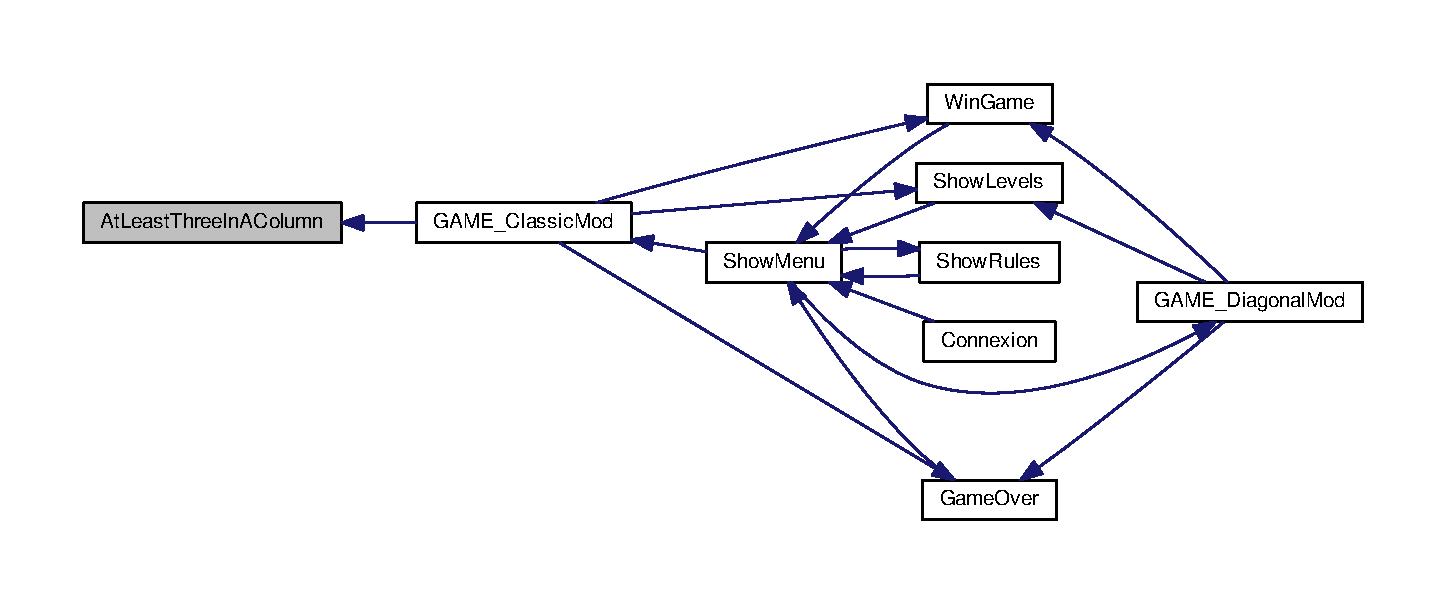
\includegraphics[width=350pt]{ingame_8h_a108e24a88952cbfc5db26c2d1fef4633_icgraph}
\end{center}
\end{figure}


\hypertarget{ingame_8h_a4a09f89d72703bc9b9fc08c19781e80b}{\index{ingame.\+h@{ingame.\+h}!At\+Least\+Three\+In\+A\+Diagonal\+Nord\+Est@{At\+Least\+Three\+In\+A\+Diagonal\+Nord\+Est}}
\index{At\+Least\+Three\+In\+A\+Diagonal\+Nord\+Est@{At\+Least\+Three\+In\+A\+Diagonal\+Nord\+Est}!ingame.\+h@{ingame.\+h}}
\subsubsection[{At\+Least\+Three\+In\+A\+Diagonal\+Nord\+Est}]{\setlength{\rightskip}{0pt plus 5cm}bool At\+Least\+Three\+In\+A\+Diagonal\+Nord\+Est (
\begin{DoxyParamCaption}
\item[{const C\+Mat \&}]{Grid, }
\item[{C\+Position \&}]{Pos, }
\item[{unsigned \&}]{How\+Many}
\end{DoxyParamCaption}
)}}\label{ingame_8h_a4a09f89d72703bc9b9fc08c19781e80b}


At\+Least\+Three\+In\+A\+Diagonal\+Nord\+Est. 


\begin{DoxyParams}{Parameters}
{\em Grid\mbox{[}in\mbox{]}} & Grille contenant les nombres \\
\hline
{\em Pos\mbox{[}in,out\mbox{]}} & Contient la position de la case sélectionnée par l'utilisateur \\
\hline
{\em How\+Many\mbox{[}in,out\mbox{]}} & Variable qui contient le nombre de même nombres alignés\mbox{[}in\mbox{]} Variable qui contient le nombre de même nombres alignés \\
\hline
\end{DoxyParams}
\begin{DoxyReturn}{Returns}
booléen qui détermine s'il reste encore des séries de nombres alignés 
\end{DoxyReturn}


Definition at line 114 of file ingame.\+cpp.



Here is the caller graph for this function\+:
\nopagebreak
\begin{figure}[H]
\begin{center}
\leavevmode
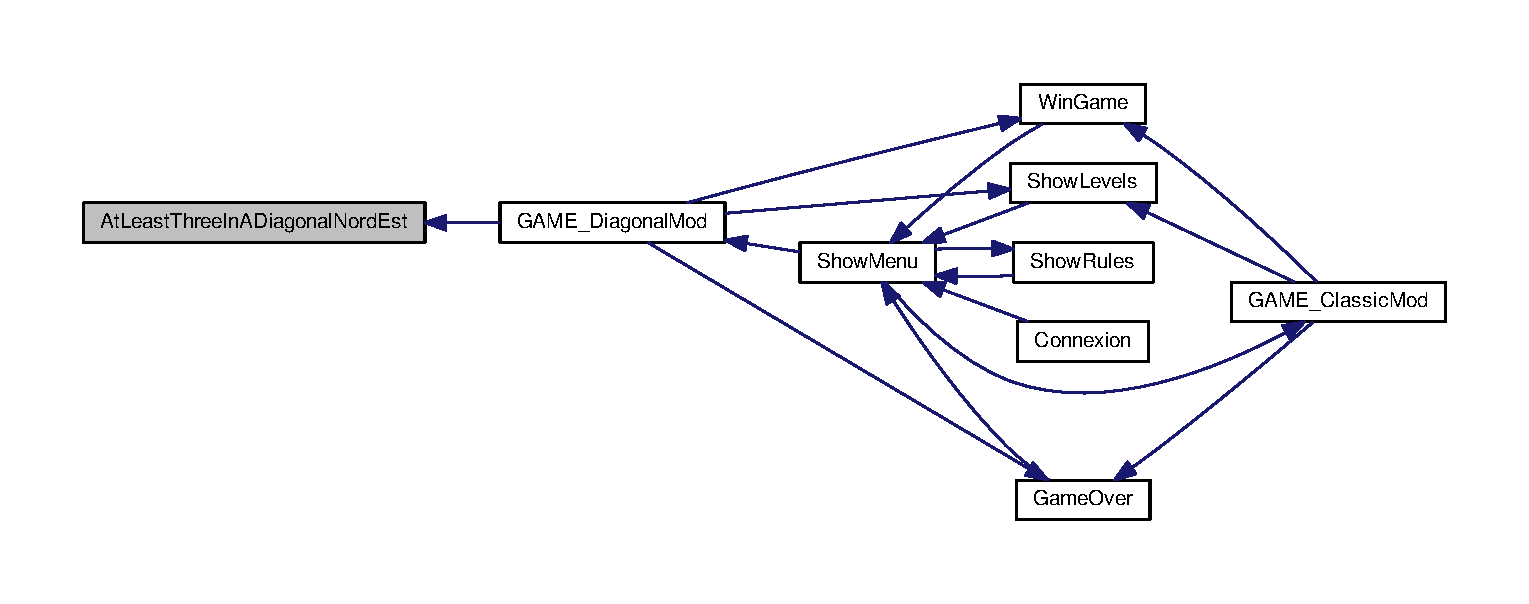
\includegraphics[width=350pt]{ingame_8h_a4a09f89d72703bc9b9fc08c19781e80b_icgraph}
\end{center}
\end{figure}


\hypertarget{ingame_8h_afee55318480451016786e0433af2faa2}{\index{ingame.\+h@{ingame.\+h}!At\+Least\+Three\+In\+A\+Diagonal\+Nord\+Ouest@{At\+Least\+Three\+In\+A\+Diagonal\+Nord\+Ouest}}
\index{At\+Least\+Three\+In\+A\+Diagonal\+Nord\+Ouest@{At\+Least\+Three\+In\+A\+Diagonal\+Nord\+Ouest}!ingame.\+h@{ingame.\+h}}
\subsubsection[{At\+Least\+Three\+In\+A\+Diagonal\+Nord\+Ouest}]{\setlength{\rightskip}{0pt plus 5cm}bool At\+Least\+Three\+In\+A\+Diagonal\+Nord\+Ouest (
\begin{DoxyParamCaption}
\item[{const C\+Mat \&}]{Grid, }
\item[{C\+Position \&}]{Pos, }
\item[{unsigned \&}]{How\+Many}
\end{DoxyParamCaption}
)}}\label{ingame_8h_afee55318480451016786e0433af2faa2}


At\+Least\+Three\+In\+A\+Diagonal\+Nord\+Ouest. 


\begin{DoxyParams}{Parameters}
{\em Grid\mbox{[}in\mbox{]}} & Grille contenant les nombres \\
\hline
{\em Pos\mbox{[}in,out\mbox{]}} & Contient la position de la case sélectionnée par l'utilisateur \\
\hline
{\em How\+Many\mbox{[}in,out\mbox{]}} & Variable qui contient le nombre de même nombres alignés \\
\hline
\end{DoxyParams}
\begin{DoxyReturn}{Returns}
booléen qui détermine s'il reste encore des séries de nombres alignés 
\end{DoxyReturn}


Definition at line 146 of file ingame.\+cpp.



Here is the caller graph for this function\+:
\nopagebreak
\begin{figure}[H]
\begin{center}
\leavevmode
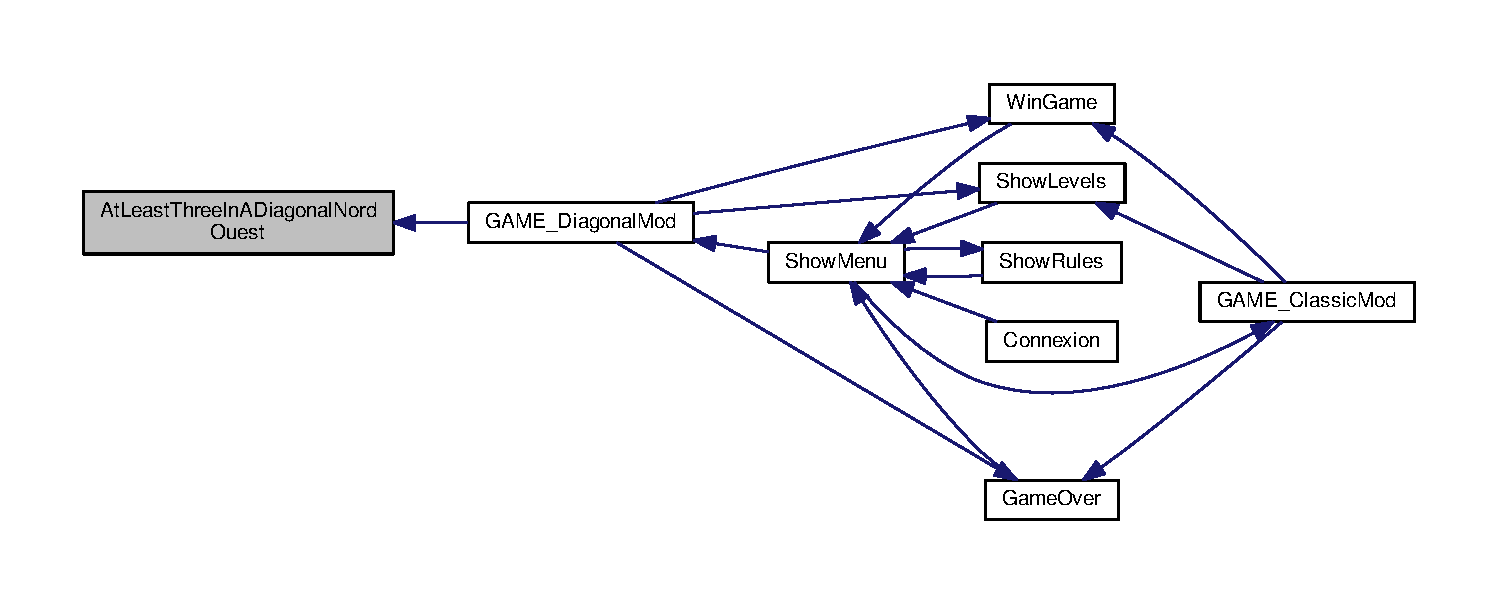
\includegraphics[width=350pt]{ingame_8h_afee55318480451016786e0433af2faa2_icgraph}
\end{center}
\end{figure}


\hypertarget{ingame_8h_ab13e1001573be4964b0b6b28f53b904b}{\index{ingame.\+h@{ingame.\+h}!At\+Least\+Three\+In\+A\+Row@{At\+Least\+Three\+In\+A\+Row}}
\index{At\+Least\+Three\+In\+A\+Row@{At\+Least\+Three\+In\+A\+Row}!ingame.\+h@{ingame.\+h}}
\subsubsection[{At\+Least\+Three\+In\+A\+Row}]{\setlength{\rightskip}{0pt plus 5cm}bool At\+Least\+Three\+In\+A\+Row (
\begin{DoxyParamCaption}
\item[{C\+Mat \&}]{Grid, }
\item[{C\+Position \&}]{Pos, }
\item[{unsigned \&}]{How\+Many, }
\item[{unsigned \&}]{Saved\+Number}
\end{DoxyParamCaption}
)}}\label{ingame_8h_ab13e1001573be4964b0b6b28f53b904b}


At\+Least\+Three\+In\+A\+Row. 


\begin{DoxyParams}{Parameters}
{\em Grid\mbox{[}in\mbox{]}} & Grille contenant les nombres \\
\hline
{\em Pos\mbox{[}in,out\mbox{]}} & Contient la position de la case sélectionnée par l'utilisateur \\
\hline
{\em How\+Many\mbox{[}in,out\mbox{]}} & Variable qui contient le nombre de même nombres alignés \\
\hline
{\em Saved\+Number\mbox{[}in,out\mbox{]}} & Nombre sauvegardé à chaque début de série puis remplacé en fin de série par le prochain nombre différent de celui sauvegardé\mbox{[}in,out\mbox{]} Nombre sauvegardé à chaque début de série puis remplacé en fin de série par le prochain nombre différent de celui sauvegardé \\
\hline
\end{DoxyParams}
\begin{DoxyReturn}{Returns}
booléen qui détermine s'il reste encore des séries de nombres alignés 
\end{DoxyReturn}


Definition at line 179 of file ingame.\+cpp.



Here is the caller graph for this function\+:
\nopagebreak
\begin{figure}[H]
\begin{center}
\leavevmode
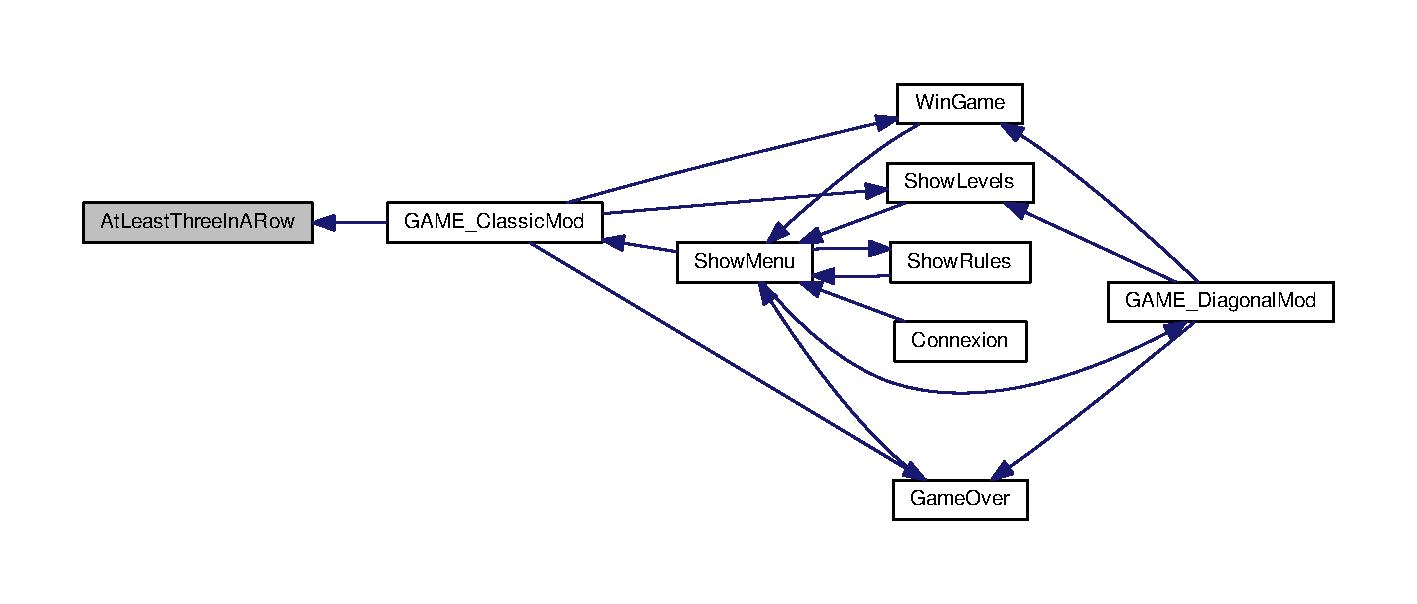
\includegraphics[width=350pt]{ingame_8h_ab13e1001573be4964b0b6b28f53b904b_icgraph}
\end{center}
\end{figure}


\hypertarget{ingame_8h_aff5ba4e81140f59295776e2f739d34ec}{\index{ingame.\+h@{ingame.\+h}!Calc\+Percentage@{Calc\+Percentage}}
\index{Calc\+Percentage@{Calc\+Percentage}!ingame.\+h@{ingame.\+h}}
\subsubsection[{Calc\+Percentage}]{\setlength{\rightskip}{0pt plus 5cm}unsigned Calc\+Percentage (
\begin{DoxyParamCaption}
\item[{int \&}]{Score\+For\+Next\+Lvl, }
\item[{int \&}]{Score}
\end{DoxyParamCaption}
)}}\label{ingame_8h_aff5ba4e81140f59295776e2f739d34ec}


Calc\+Percentage. 


\begin{DoxyParams}{Parameters}
{\em Score\+For\+Next\+Lvl\mbox{[}in\mbox{]}} & Score à atteindre pour gagner le niveau \\
\hline
{\em Score\mbox{[}in\mbox{]}} & Score du joueur \\
\hline
\end{DoxyParams}


Definition at line 262 of file ingame.\+cpp.



Here is the caller graph for this function\+:
\nopagebreak
\begin{figure}[H]
\begin{center}
\leavevmode
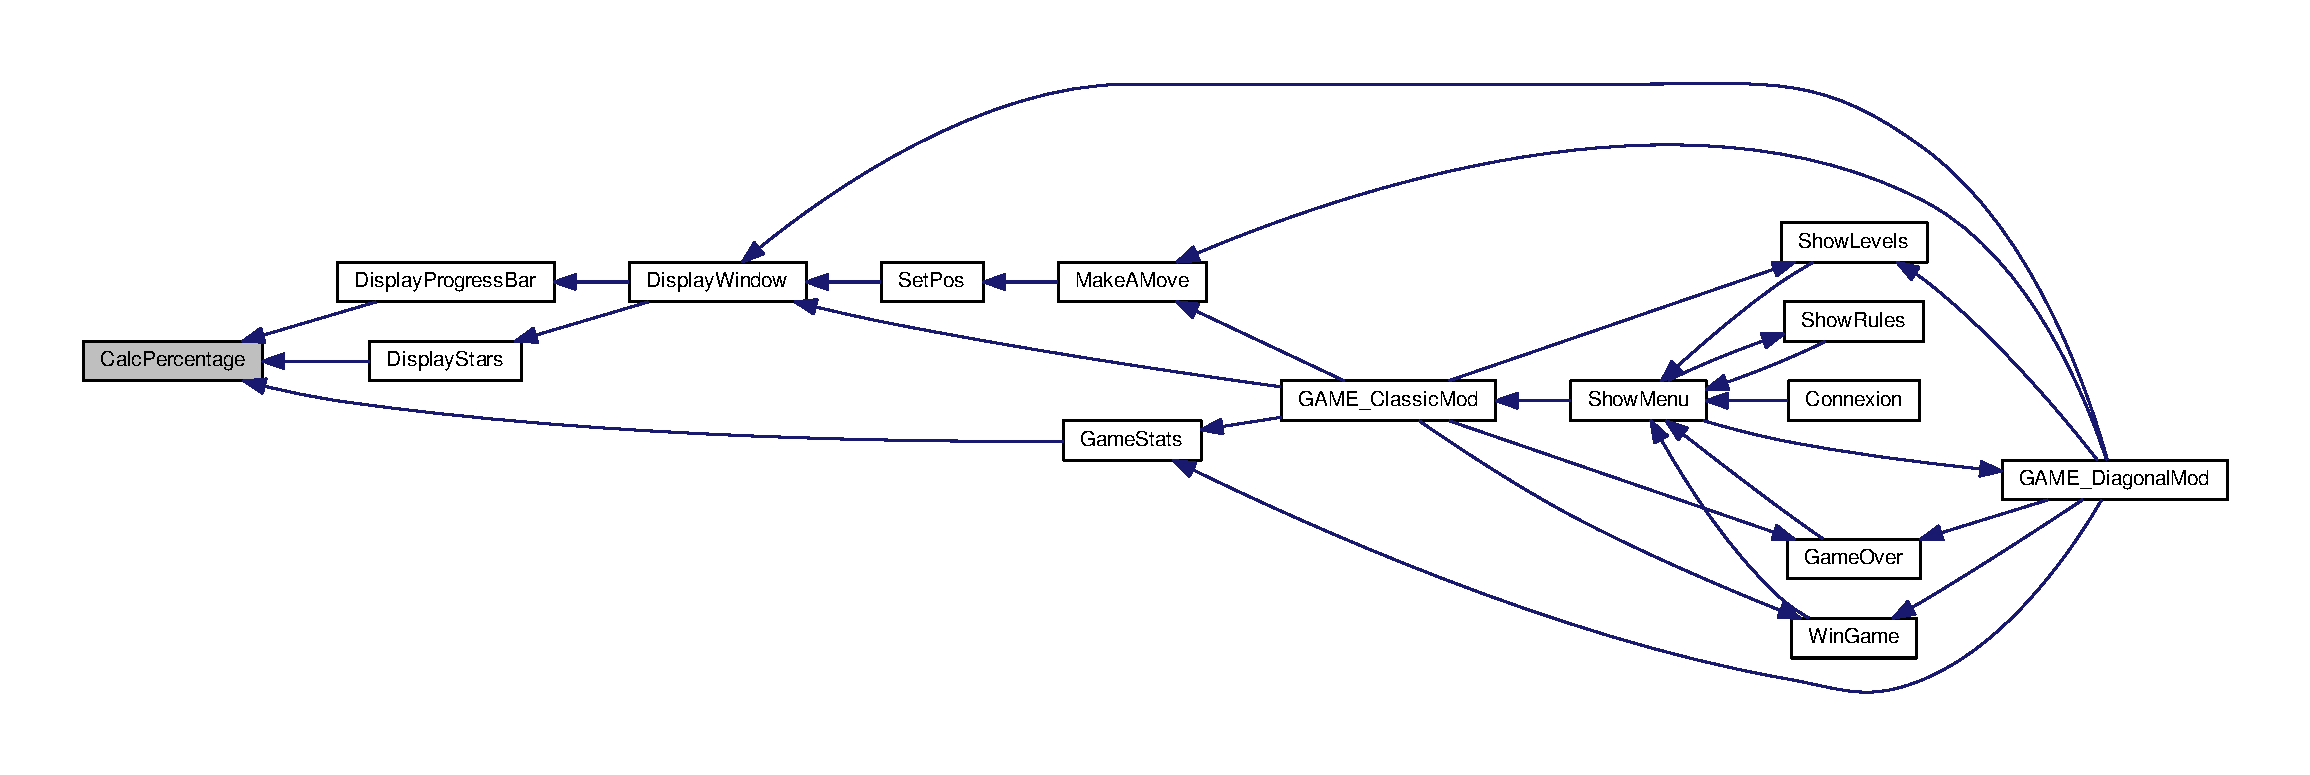
\includegraphics[width=350pt]{ingame_8h_aff5ba4e81140f59295776e2f739d34ec_icgraph}
\end{center}
\end{figure}


\hypertarget{ingame_8h_ad02fc64961716c22249708018aa1da56}{\index{ingame.\+h@{ingame.\+h}!Check\+New\+Record@{Check\+New\+Record}}
\index{Check\+New\+Record@{Check\+New\+Record}!ingame.\+h@{ingame.\+h}}
\subsubsection[{Check\+New\+Record}]{\setlength{\rightskip}{0pt plus 5cm}void Check\+New\+Record (
\begin{DoxyParamCaption}
\item[{C\+Mat\+Str \&}]{Leader\+Board, }
\item[{int \&}]{Score, }
\item[{int \&}]{Game\+Choice, }
\item[{int \&}]{Level\+Choice, }
\item[{const string \&}]{Pseudo}
\end{DoxyParamCaption}
)}}\label{ingame_8h_ad02fc64961716c22249708018aa1da56}


Check\+New\+Record. 


\begin{DoxyParams}{Parameters}
{\em Leader\+Board\mbox{[}in,out\mbox{]}} & Matrice contenant l'ensemble des scores des joueurs pour chaque niveau \\
\hline
{\em Score\mbox{[}in\mbox{]}} & Score du joueur \\
\hline
{\em Game\+Choice\mbox{[}in\mbox{]}} & Mode de jeu choisi par l'utilisateur \\
\hline
{\em Level\+Choice\mbox{[}in\mbox{]}} & Level choisi par l'utilisateur \\
\hline
{\em Pseudo\mbox{[}in\mbox{]}} & Pseudo du joueur entré au début du jeu \\
\hline
\end{DoxyParams}


Definition at line 280 of file ingame.\+cpp.



Here is the caller graph for this function\+:
\nopagebreak
\begin{figure}[H]
\begin{center}
\leavevmode
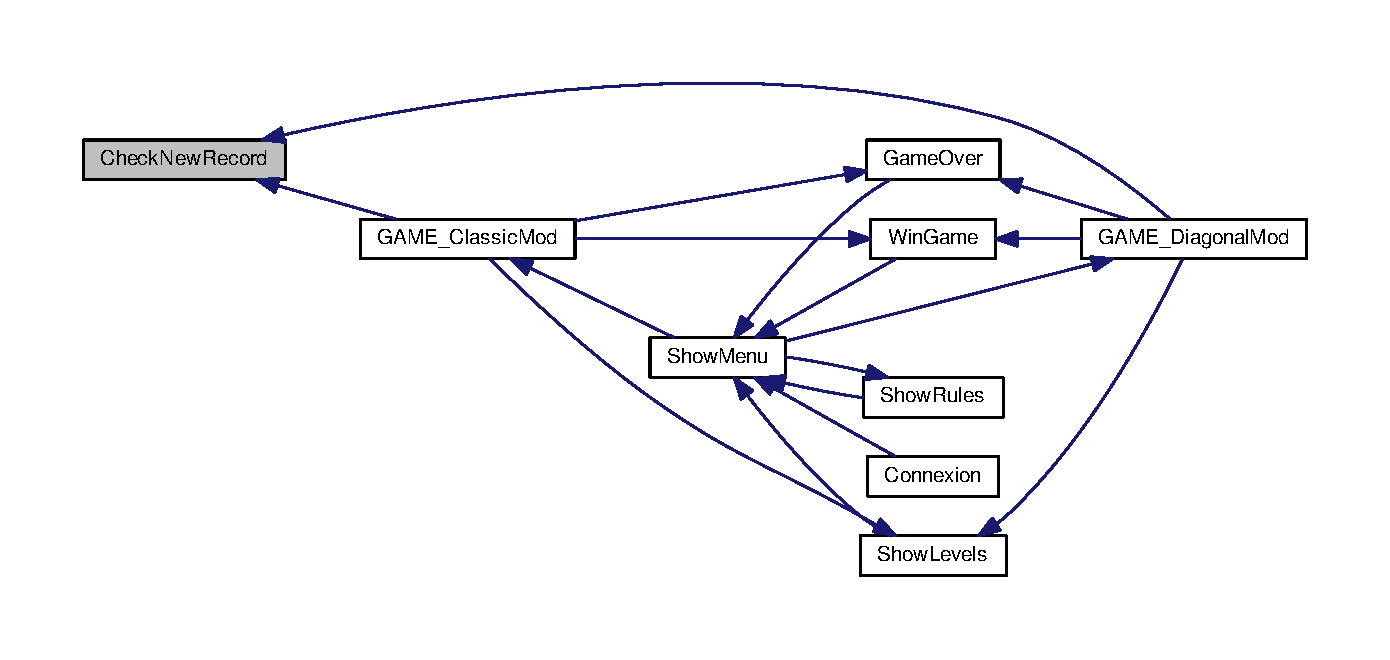
\includegraphics[width=350pt]{ingame_8h_ad02fc64961716c22249708018aa1da56_icgraph}
\end{center}
\end{figure}


\hypertarget{ingame_8h_a357e1a065c7e8aebe8cc1df46ce31a28}{\index{ingame.\+h@{ingame.\+h}!Game\+Stats@{Game\+Stats}}
\index{Game\+Stats@{Game\+Stats}!ingame.\+h@{ingame.\+h}}
\subsubsection[{Game\+Stats}]{\setlength{\rightskip}{0pt plus 5cm}string Game\+Stats (
\begin{DoxyParamCaption}
\item[{int \&}]{Score\+For\+Next\+Lvl, }
\item[{int \&}]{Score, }
\item[{int \&}]{Maximal\+Hits, }
\item[{int \&}]{Hits}
\end{DoxyParamCaption}
)}}\label{ingame_8h_a357e1a065c7e8aebe8cc1df46ce31a28}


Game\+Stats. 


\begin{DoxyParams}{Parameters}
{\em Score\+For\+Next\+Lvl\mbox{[}in\mbox{]}} & Score à atteindre pour gagner le niveau \\
\hline
{\em Score\mbox{[}in\mbox{]}} & Score du joueur \\
\hline
{\em Maximal\+Hits\mbox{[}in\mbox{]}} & Nombre maximum de coups attribués pour le level \\
\hline
{\em Hits\mbox{[}in\mbox{]}} & Nombre de coups utilisés \\
\hline
\end{DoxyParams}
\begin{DoxyReturn}{Returns}
string qui permet de savoir si le joueur à perdu, gagné, ou s'il peut toujours continuer à jouer 
\end{DoxyReturn}


Definition at line 273 of file ingame.\+cpp.



Here is the call graph for this function\+:
\nopagebreak
\begin{figure}[H]
\begin{center}
\leavevmode
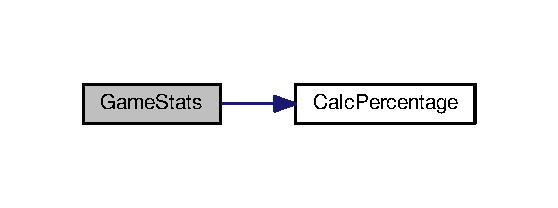
\includegraphics[width=268pt]{ingame_8h_a357e1a065c7e8aebe8cc1df46ce31a28_cgraph}
\end{center}
\end{figure}




Here is the caller graph for this function\+:
\nopagebreak
\begin{figure}[H]
\begin{center}
\leavevmode
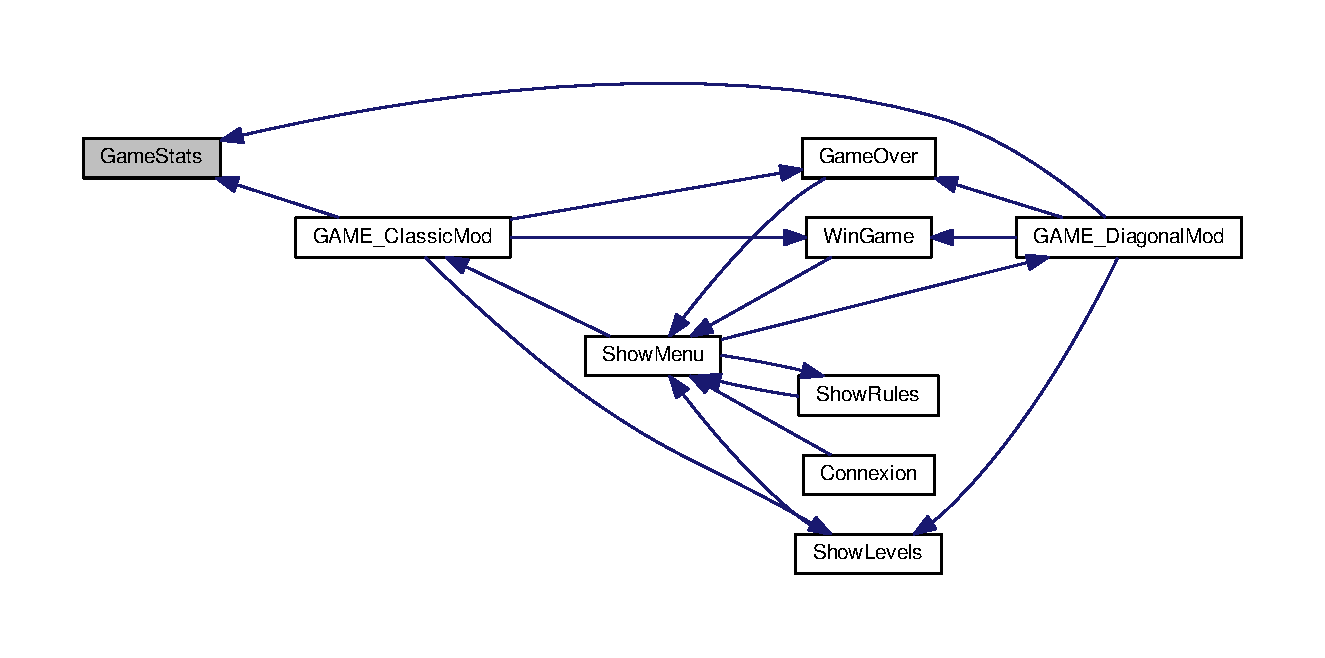
\includegraphics[width=350pt]{ingame_8h_a357e1a065c7e8aebe8cc1df46ce31a28_icgraph}
\end{center}
\end{figure}


\hypertarget{ingame_8h_a60837ded3ac39240259c93509f783ba8}{\index{ingame.\+h@{ingame.\+h}!Make\+A\+Move@{Make\+A\+Move}}
\index{Make\+A\+Move@{Make\+A\+Move}!ingame.\+h@{ingame.\+h}}
\subsubsection[{Make\+A\+Move}]{\setlength{\rightskip}{0pt plus 5cm}void Make\+A\+Move (
\begin{DoxyParamCaption}
\item[{C\+Mat \&}]{Grid, }
\item[{C\+Position \&}]{Pos, }
\item[{char \&}]{Direction, }
\item[{bool \&}]{Next\+Number, }
\item[{const C\+Mat\+Str \&}]{Leader\+Board, }
\item[{int \&}]{Score\+For\+Next\+Lvl, }
\item[{int \&}]{Score, }
\item[{int \&}]{Level\+Choice, }
\item[{int \&}]{Maximal\+Hits, }
\item[{int \&}]{Hits}
\end{DoxyParamCaption}
)}}\label{ingame_8h_a60837ded3ac39240259c93509f783ba8}


Make\+A\+Move. 


\begin{DoxyParams}{Parameters}
{\em Grid\mbox{[}in\mbox{]}} & Grille contenant les nombres \\
\hline
{\em Pos\mbox{[}in\mbox{]}} & Contient la position de la case sélectionnée par l'utilisateur \\
\hline
{\em Direction\mbox{[}in\mbox{]}} & Caractère contenant la direction choisie \\
\hline
{\em Next\+Number\mbox{[}in,out\mbox{]}} & Booléen qui vérifie si le nombre a bien été échangé \\
\hline
{\em Leader\+Board\mbox{[}in\mbox{]}} & Matrice contenant l'ensemble des scores des joueurs pour chaque niveau \\
\hline
{\em Score\+For\+Next\+Lvl\mbox{[}in\mbox{]}} & Score à atteindre pour gagner le niveau \\
\hline
{\em Score\mbox{[}in\mbox{]}} & Score du joueur \\
\hline
{\em Level\+Choice\mbox{[}in\mbox{]}} & Level choisi par l'utilisateur \\
\hline
{\em Maximal\+Hits\mbox{[}in\mbox{]}} & Nombre maximum de coups attribués pour le level \\
\hline
{\em Hits\mbox{[}in\mbox{]}} & Nombre de coups utilisés \\
\hline
\end{DoxyParams}


Definition at line 88 of file ingame.\+cpp.



Here is the call graph for this function\+:
\nopagebreak
\begin{figure}[H]
\begin{center}
\leavevmode
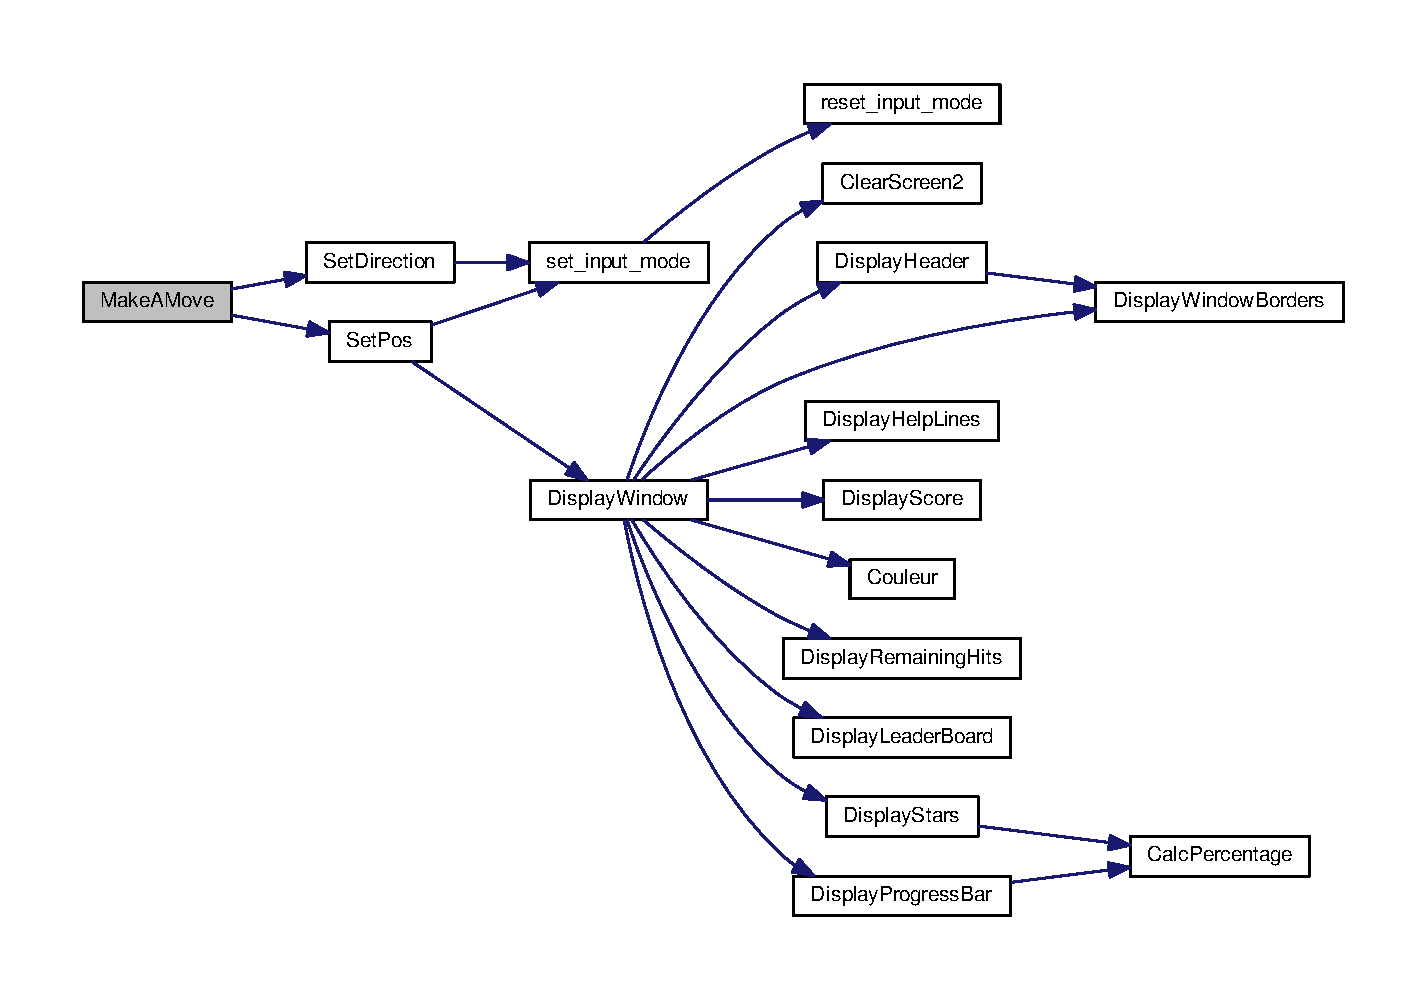
\includegraphics[width=350pt]{ingame_8h_a60837ded3ac39240259c93509f783ba8_cgraph}
\end{center}
\end{figure}




Here is the caller graph for this function\+:
\nopagebreak
\begin{figure}[H]
\begin{center}
\leavevmode
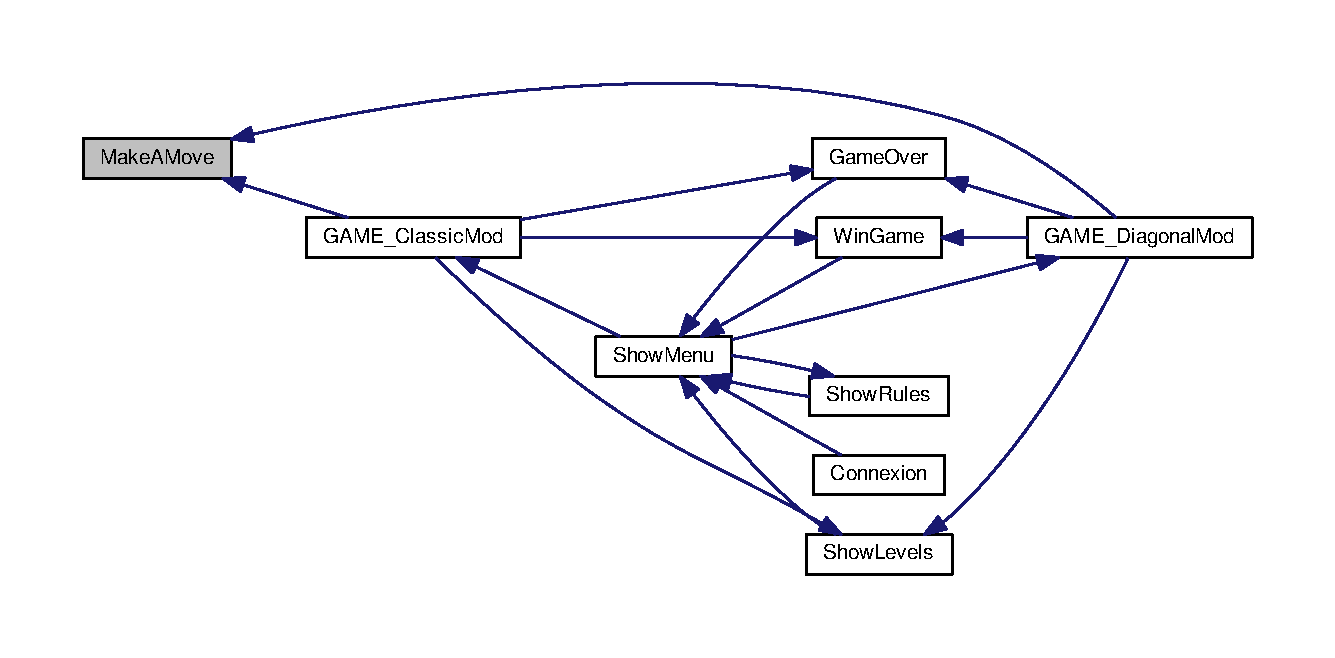
\includegraphics[width=350pt]{ingame_8h_a60837ded3ac39240259c93509f783ba8_icgraph}
\end{center}
\end{figure}


\hypertarget{ingame_8h_ae08a929793a9f09a17e40cc361e4f1b6}{\index{ingame.\+h@{ingame.\+h}!Removal\+In\+Column@{Removal\+In\+Column}}
\index{Removal\+In\+Column@{Removal\+In\+Column}!ingame.\+h@{ingame.\+h}}
\subsubsection[{Removal\+In\+Column}]{\setlength{\rightskip}{0pt plus 5cm}void Removal\+In\+Column (
\begin{DoxyParamCaption}
\item[{C\+Mat \&}]{Grid, }
\item[{const C\+Position \&}]{Pos, }
\item[{unsigned \&}]{How\+Many}
\end{DoxyParamCaption}
)}}\label{ingame_8h_ae08a929793a9f09a17e40cc361e4f1b6}


Removal\+In\+Column. 


\begin{DoxyParams}{Parameters}
{\em Grid\mbox{[}in,out\mbox{]}} & Grille contenant les nombres \\
\hline
{\em Pos\mbox{[}in\mbox{]}} & Contient la position de la case sélectionnée par l'utilisateur \\
\hline
{\em How\+Many\mbox{[}in\mbox{]}} & Variable qui contient le nombre de même nombres alignés \\
\hline
\end{DoxyParams}


Definition at line 204 of file ingame.\+cpp.



Here is the caller graph for this function\+:
\nopagebreak
\begin{figure}[H]
\begin{center}
\leavevmode
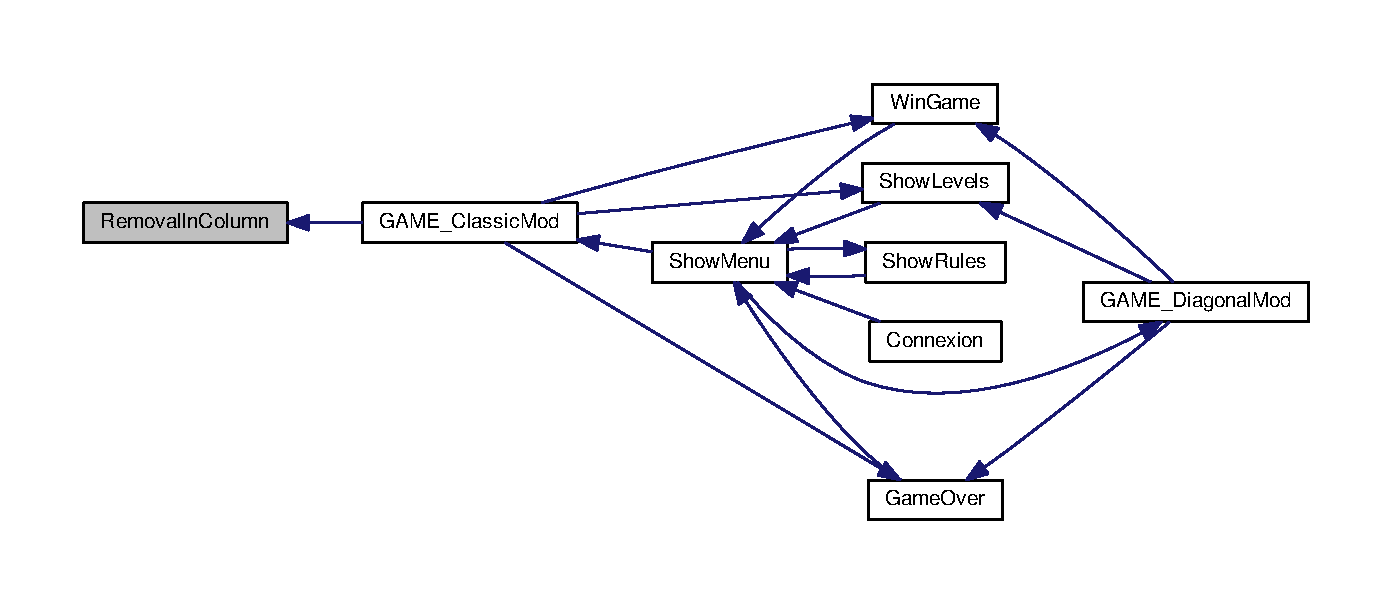
\includegraphics[width=350pt]{ingame_8h_ae08a929793a9f09a17e40cc361e4f1b6_icgraph}
\end{center}
\end{figure}


\hypertarget{ingame_8h_a3782b9c91c01c218dd60721fa091a274}{\index{ingame.\+h@{ingame.\+h}!Removal\+In\+Diagonal\+Nord\+Est@{Removal\+In\+Diagonal\+Nord\+Est}}
\index{Removal\+In\+Diagonal\+Nord\+Est@{Removal\+In\+Diagonal\+Nord\+Est}!ingame.\+h@{ingame.\+h}}
\subsubsection[{Removal\+In\+Diagonal\+Nord\+Est}]{\setlength{\rightskip}{0pt plus 5cm}void Removal\+In\+Diagonal\+Nord\+Est (
\begin{DoxyParamCaption}
\item[{C\+Mat \&}]{Grid, }
\item[{const C\+Position \&}]{Pos, }
\item[{unsigned \&}]{How\+Many}
\end{DoxyParamCaption}
)}}\label{ingame_8h_a3782b9c91c01c218dd60721fa091a274}


Removal\+In\+Diagonal\+Nord\+Est. 


\begin{DoxyParams}{Parameters}
{\em Grid\mbox{[}in,out\mbox{]}} & Grille contenant les nombres \\
\hline
{\em Pos\mbox{[}in\mbox{]}} & Contient la position de la case sélectionnée par l'utilisateur \\
\hline
{\em How\+Many\mbox{[}in\mbox{]}} & Variable qui contient le nombre de même nombres alignés\mbox{[}in\mbox{]} Variable qui contient le nombre de même nombres alignés \\
\hline
\end{DoxyParams}


Definition at line 102 of file ingame.\+cpp.



Here is the caller graph for this function\+:
\nopagebreak
\begin{figure}[H]
\begin{center}
\leavevmode
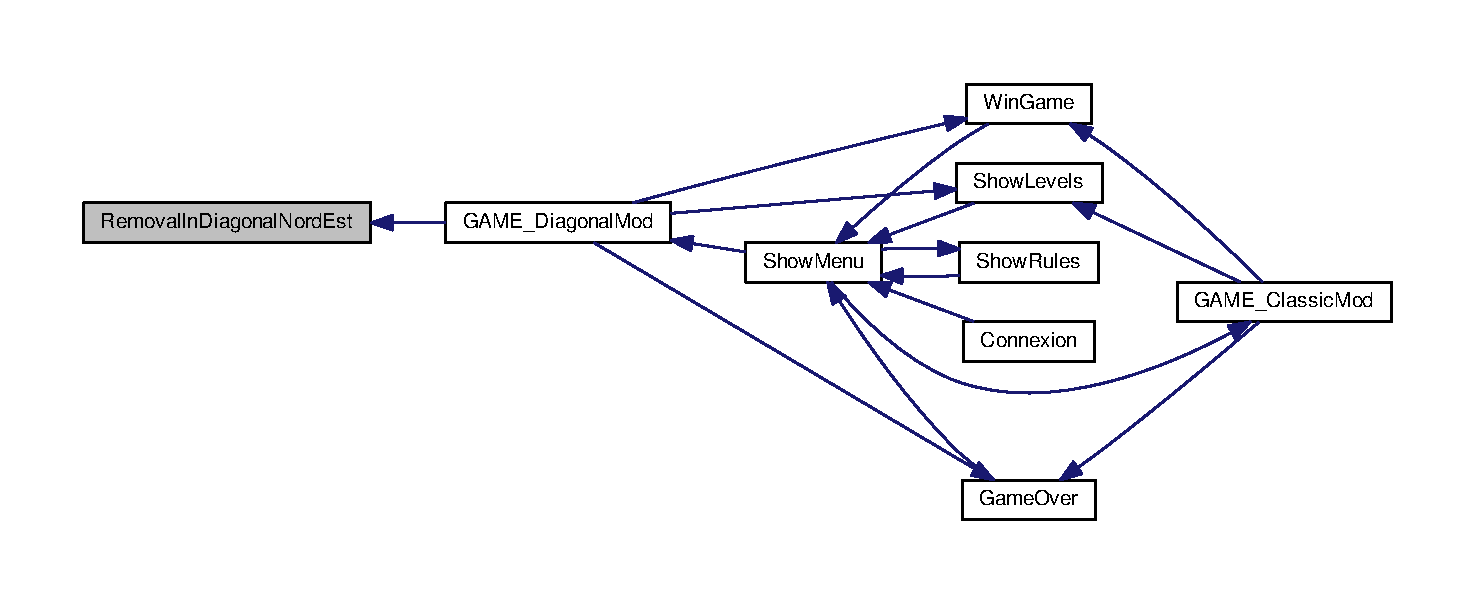
\includegraphics[width=350pt]{ingame_8h_a3782b9c91c01c218dd60721fa091a274_icgraph}
\end{center}
\end{figure}


\hypertarget{ingame_8h_aabc4dce46a5efcd51f169098ba015727}{\index{ingame.\+h@{ingame.\+h}!Removal\+In\+Diagonal\+Nord\+Ouest@{Removal\+In\+Diagonal\+Nord\+Ouest}}
\index{Removal\+In\+Diagonal\+Nord\+Ouest@{Removal\+In\+Diagonal\+Nord\+Ouest}!ingame.\+h@{ingame.\+h}}
\subsubsection[{Removal\+In\+Diagonal\+Nord\+Ouest}]{\setlength{\rightskip}{0pt plus 5cm}void Removal\+In\+Diagonal\+Nord\+Ouest (
\begin{DoxyParamCaption}
\item[{C\+Mat \&}]{Grid, }
\item[{const C\+Position \&}]{Pos, }
\item[{unsigned \&}]{How\+Many}
\end{DoxyParamCaption}
)}}\label{ingame_8h_aabc4dce46a5efcd51f169098ba015727}


Removal\+In\+Diagonal\+Nord\+Ouest. 


\begin{DoxyParams}{Parameters}
{\em Grid\mbox{[}in,out\mbox{]}} & Grille contenant les nombres \\
\hline
{\em Pos\mbox{[}in\mbox{]}} & Contient la position de la case sélectionnée par l'utilisateur \\
\hline
{\em How\+Many\mbox{[}in\mbox{]}} & Variable qui contient le nombre de même nombres alignés \\
\hline
\end{DoxyParams}


Definition at line 134 of file ingame.\+cpp.



Here is the caller graph for this function\+:
\nopagebreak
\begin{figure}[H]
\begin{center}
\leavevmode
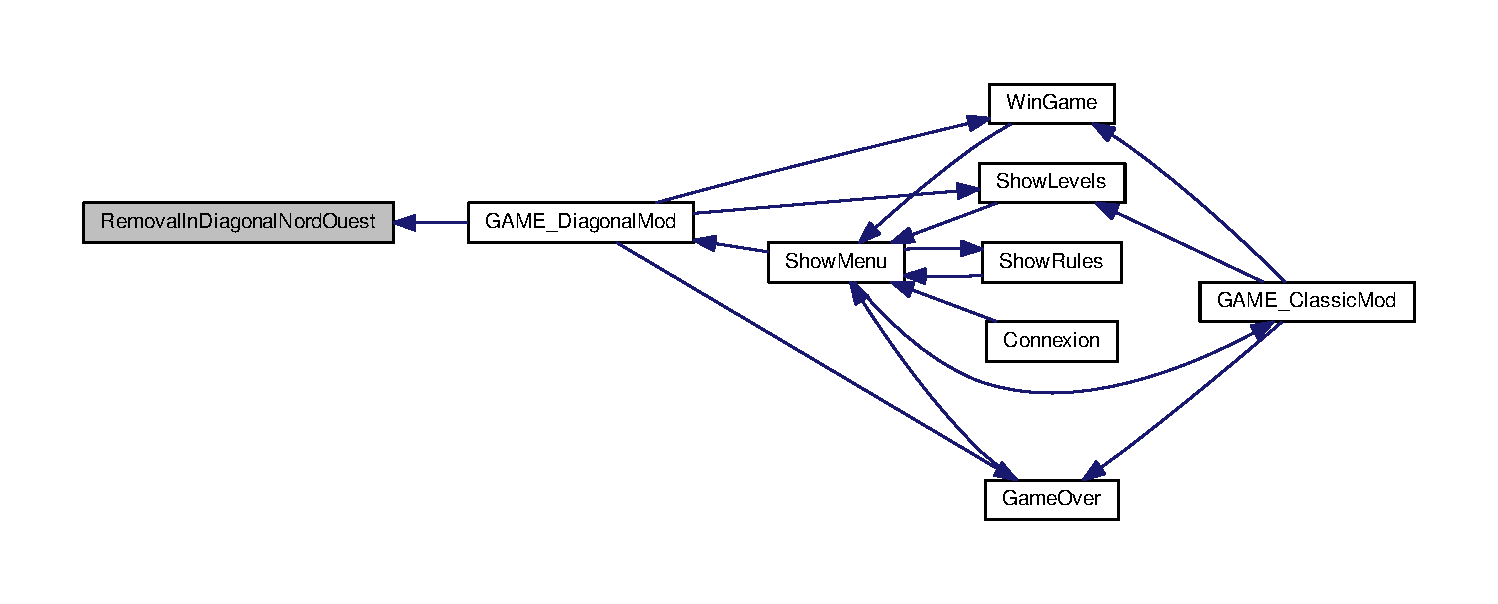
\includegraphics[width=350pt]{ingame_8h_aabc4dce46a5efcd51f169098ba015727_icgraph}
\end{center}
\end{figure}


\hypertarget{ingame_8h_a5ca54be49179a28392f4ca76639ea63f}{\index{ingame.\+h@{ingame.\+h}!Replace\+K\+Impossible\+Numbers@{Replace\+K\+Impossible\+Numbers}}
\index{Replace\+K\+Impossible\+Numbers@{Replace\+K\+Impossible\+Numbers}!ingame.\+h@{ingame.\+h}}
\subsubsection[{Replace\+K\+Impossible\+Numbers}]{\setlength{\rightskip}{0pt plus 5cm}void Replace\+K\+Impossible\+Numbers (
\begin{DoxyParamCaption}
\item[{C\+Mat \&}]{Grid}
\end{DoxyParamCaption}
)}}\label{ingame_8h_a5ca54be49179a28392f4ca76639ea63f}


Replace\+K\+Impossible\+Numbers. 


\begin{DoxyParams}{Parameters}
{\em Grid\mbox{[}in,out\mbox{]}} & Grille contenant les nombres \\
\hline
\end{DoxyParams}


Definition at line 240 of file ingame.\+cpp.



Here is the caller graph for this function\+:
\nopagebreak
\begin{figure}[H]
\begin{center}
\leavevmode
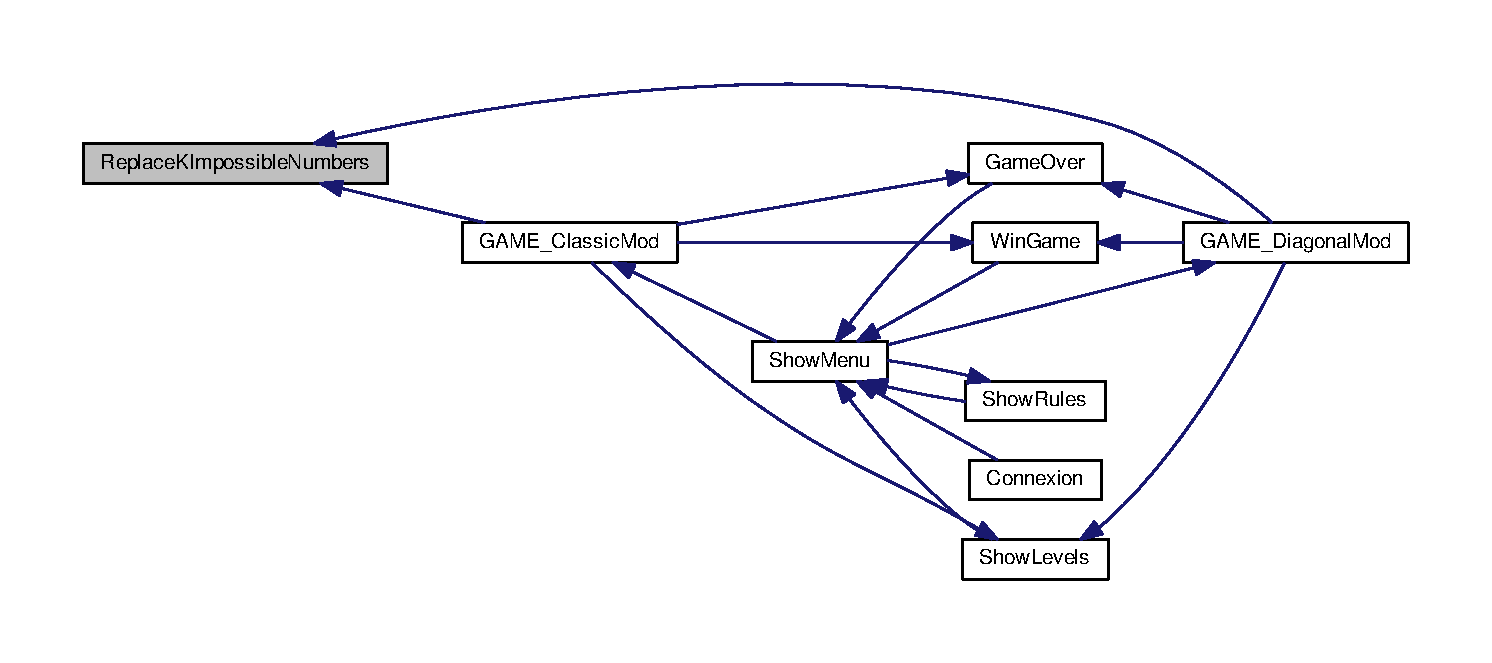
\includegraphics[width=350pt]{ingame_8h_a5ca54be49179a28392f4ca76639ea63f_icgraph}
\end{center}
\end{figure}


\hypertarget{ingame_8h_a295fed03353e3a7d18d3a64a572b99ec}{\index{ingame.\+h@{ingame.\+h}!Set\+Direction@{Set\+Direction}}
\index{Set\+Direction@{Set\+Direction}!ingame.\+h@{ingame.\+h}}
\subsubsection[{Set\+Direction}]{\setlength{\rightskip}{0pt plus 5cm}void Set\+Direction (
\begin{DoxyParamCaption}
\item[{C\+Mat \&}]{Grid, }
\item[{C\+Position \&}]{Pos, }
\item[{char \&}]{Direction, }
\item[{bool \&}]{Next\+Number}
\end{DoxyParamCaption}
)}}\label{ingame_8h_a295fed03353e3a7d18d3a64a572b99ec}


Set\+Direction permet de choisir la directionn souhaitée (haut, bas , gauche, droite) 


\begin{DoxyParams}{Parameters}
{\em Grid\mbox{[}in\mbox{]}} & Grille contenant les nombres \\
\hline
{\em Pos\mbox{[}in\mbox{]}} & Contient la position de la case sélectionnée par l'utilisateur \\
\hline
{\em Direction\mbox{[}in,out\mbox{]}} & Caractère contenant la direction choisie \\
\hline
{\em Next\+Number\mbox{[}in,out\mbox{]}} & Booléen qui vérifie si le nombre a bien été échangé \\
\hline
\end{DoxyParams}


Definition at line 41 of file ingame.\+cpp.



Here is the call graph for this function\+:
\nopagebreak
\begin{figure}[H]
\begin{center}
\leavevmode
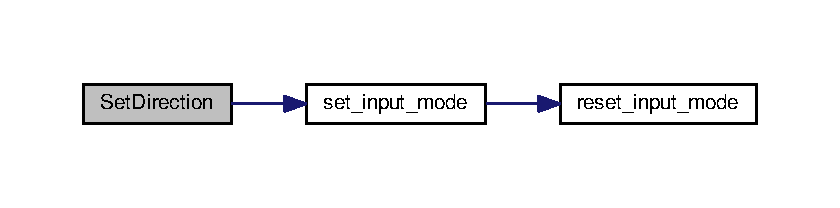
\includegraphics[width=350pt]{ingame_8h_a295fed03353e3a7d18d3a64a572b99ec_cgraph}
\end{center}
\end{figure}




Here is the caller graph for this function\+:
\nopagebreak
\begin{figure}[H]
\begin{center}
\leavevmode
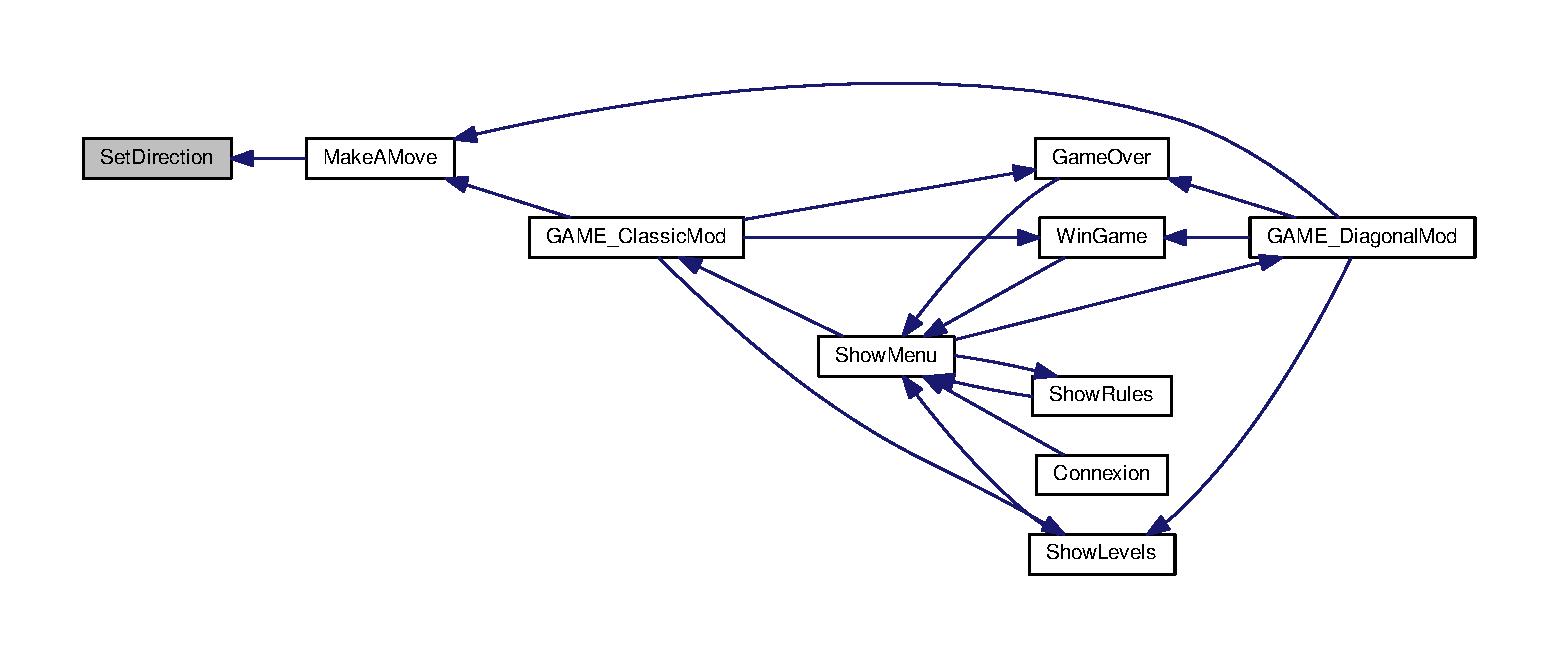
\includegraphics[width=350pt]{ingame_8h_a295fed03353e3a7d18d3a64a572b99ec_icgraph}
\end{center}
\end{figure}


\hypertarget{ingame_8h_afbd1bef0eeee45e421b3578f66acba35}{\index{ingame.\+h@{ingame.\+h}!Set\+Pos@{Set\+Pos}}
\index{Set\+Pos@{Set\+Pos}!ingame.\+h@{ingame.\+h}}
\subsubsection[{Set\+Pos}]{\setlength{\rightskip}{0pt plus 5cm}void Set\+Pos (
\begin{DoxyParamCaption}
\item[{C\+Position \&}]{Pos, }
\item[{const C\+Mat \&}]{Grid, }
\item[{const C\+Mat\+Str \&}]{Leader\+Board, }
\item[{int \&}]{Score\+For\+Next\+Lvl, }
\item[{int \&}]{Score, }
\item[{int \&}]{Level\+Choice, }
\item[{int \&}]{Maximal\+Hits, }
\item[{int \&}]{Hits}
\end{DoxyParamCaption}
)}}\label{ingame_8h_afbd1bef0eeee45e421b3578f66acba35}


Set\+Pos permet de sélectionner la position horizontale et verticale de la case que l'on souhaite. 


\begin{DoxyParams}{Parameters}
{\em Pos\mbox{[}in,out\mbox{]}} & Contient la position de la case sélectionnée par l'utilisateur \\
\hline
{\em Grid\mbox{[}in\mbox{]}} & Grille contenant les nombres \\
\hline
{\em Leader\+Board\mbox{[}in\mbox{]}} & Matrice contenant l'ensemble des scores des joueurs pour chaque niveau \\
\hline
{\em Score\+For\+Next\+Lvl\mbox{[}in\mbox{]}} & Score à atteindre pour gagner le niveau \\
\hline
{\em Score\mbox{[}in\mbox{]}} & Score du joueur \\
\hline
{\em Level\+Choice\mbox{[}in\mbox{]}} & Level choisi par l'utilisateur \\
\hline
{\em Maximal\+Hits\mbox{[}in\mbox{]}} & Nombre maximum de coups attribués pour le level \\
\hline
{\em Hits\mbox{[}in\mbox{]}} & Nombre de coups utilisés \\
\hline
\end{DoxyParams}


Definition at line 8 of file ingame.\+cpp.



Here is the call graph for this function\+:
\nopagebreak
\begin{figure}[H]
\begin{center}
\leavevmode
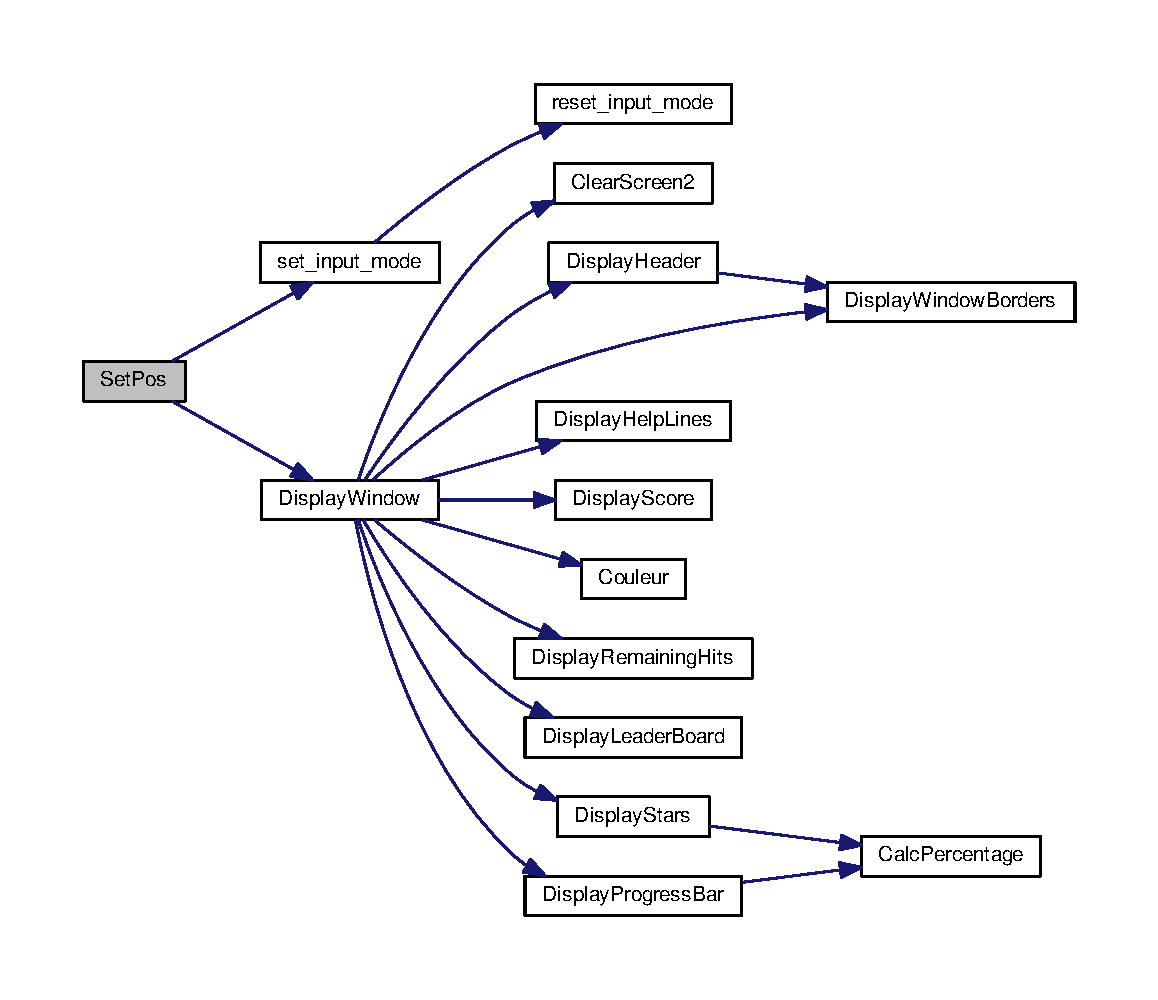
\includegraphics[width=350pt]{ingame_8h_afbd1bef0eeee45e421b3578f66acba35_cgraph}
\end{center}
\end{figure}




Here is the caller graph for this function\+:
\nopagebreak
\begin{figure}[H]
\begin{center}
\leavevmode
\includegraphics[width=350pt]{ingame_8h_afbd1bef0eeee45e421b3578f66acba35_icgraph}
\end{center}
\end{figure}


\hypertarget{ingame_8h_aa3578b144300dcc54634d4edb8aacebc}{\index{ingame.\+h@{ingame.\+h}!Update\+Score@{Update\+Score}}
\index{Update\+Score@{Update\+Score}!ingame.\+h@{ingame.\+h}}
\subsubsection[{Update\+Score}]{\setlength{\rightskip}{0pt plus 5cm}void Update\+Score (
\begin{DoxyParamCaption}
\item[{const unsigned \&}]{How\+Many, }
\item[{int \&}]{Score}
\end{DoxyParamCaption}
)}}\label{ingame_8h_aa3578b144300dcc54634d4edb8aacebc}


Update\+Score. 


\begin{DoxyParams}{Parameters}
{\em How\+Many\mbox{[}in\mbox{]}} & Variable qui contient le nombre de même nombres alignés \\
\hline
{\em Score\mbox{[}in,out\mbox{]}} & Score du joueur \\
\hline
\end{DoxyParams}


Definition at line 252 of file ingame.\+cpp.



Here is the caller graph for this function\+:
\nopagebreak
\begin{figure}[H]
\begin{center}
\leavevmode
\includegraphics[width=350pt]{ingame_8h_aa3578b144300dcc54634d4edb8aacebc_icgraph}
\end{center}
\end{figure}



\hypertarget{init_8h}{\section{init.\+h File Reference}
\label{init_8h}\index{init.\+h@{init.\+h}}
}


Fonctions d'initialisation.  


{\ttfamily \#include \char`\"{}params2.\+h\char`\"{}}\\*
Include dependency graph for init.\+h\+:
\nopagebreak
\begin{figure}[H]
\begin{center}
\leavevmode
\includegraphics[width=350pt]{init_8h__incl}
\end{center}
\end{figure}
This graph shows which files directly or indirectly include this file\+:
\nopagebreak
\begin{figure}[H]
\begin{center}
\leavevmode
\includegraphics[width=314pt]{init_8h__dep__incl}
\end{center}
\end{figure}
\subsection*{Functions}
\begin{DoxyCompactItemize}
\item 
void \hyperlink{init_8h_a69f66a6accb166c57bb7930bad085a20}{Reset\+Data} (int \&Score, int \&Game\+Choice, int \&Level\+Choice, int \&Hits)
\begin{DoxyCompactList}\small\item\em Reset\+Data reinitialise les données. \end{DoxyCompactList}\item 
void \hyperlink{init_8h_a43e6a452a6a528430946355ed0a7becb}{Init\+Grid2} (C\+Mat \&Grid, const unsigned \&Size)
\begin{DoxyCompactList}\small\item\em Init\+Grid2 génère des nombres aléatoires dans la grille. \end{DoxyCompactList}\item 
void \hyperlink{init_8h_a8417e51a7c975bc6404280ef54bdb509}{Init\+Leader\+Board} (ifstream \&ifs, C\+Mat\+Str \&Leader\+Board, int \&Game\+Choice)
\begin{DoxyCompactList}\small\item\em Init\+Leader\+Board en fonction du mode de jeu lit le fichier texte associé afin de remplir la matrice Leader\+Board avec le nom du joueur et son score. \end{DoxyCompactList}\item 
void \hyperlink{init_8h_a075b1473c05c7c715501bff357e16b32}{Check\+Grid} (C\+Mat \&Grid)
\begin{DoxyCompactList}\small\item\em Check\+Grid vérifie que la grille ne contienne pas 3 mêmes chiffres d'affilé \end{DoxyCompactList}\item 
void \hyperlink{init_8h_aa4699d640d199fc44a0c98dc6a5d45f5}{Couleur} (const string \&coul)
\begin{DoxyCompactList}\small\item\em Couleur détermine la couleur du fond de la case en fonction du chiffre. \end{DoxyCompactList}\end{DoxyCompactItemize}


\subsection{Detailed Description}
Fonctions d'initialisation. 

\begin{DoxyAuthor}{Author}
Quentin Pla, Léo Vincent, Emma tarfi, Sirine Achache, Julien Vavrille
\end{DoxyAuthor}
\begin{DoxyDate}{Date}
26 janvier 2018 
\end{DoxyDate}


Definition in file \hyperlink{init_8h_source}{init.\+h}.



\subsection{Function Documentation}
\hypertarget{init_8h_a075b1473c05c7c715501bff357e16b32}{\index{init.\+h@{init.\+h}!Check\+Grid@{Check\+Grid}}
\index{Check\+Grid@{Check\+Grid}!init.\+h@{init.\+h}}
\subsubsection[{Check\+Grid}]{\setlength{\rightskip}{0pt plus 5cm}void Check\+Grid (
\begin{DoxyParamCaption}
\item[{C\+Mat \&}]{Grid}
\end{DoxyParamCaption}
)}}\label{init_8h_a075b1473c05c7c715501bff357e16b32}


Check\+Grid vérifie que la grille ne contienne pas 3 mêmes chiffres d'affilé 


\begin{DoxyParams}{Parameters}
{\em Grid\mbox{[}in,out\mbox{]}} & Grille contenant les nombres \\
\hline
\end{DoxyParams}


Definition at line 68 of file init.\+cpp.



Here is the caller graph for this function\+:
\nopagebreak
\begin{figure}[H]
\begin{center}
\leavevmode
\includegraphics[width=350pt]{init_8h_a075b1473c05c7c715501bff357e16b32_icgraph}
\end{center}
\end{figure}


\hypertarget{init_8h_aa4699d640d199fc44a0c98dc6a5d45f5}{\index{init.\+h@{init.\+h}!Couleur@{Couleur}}
\index{Couleur@{Couleur}!init.\+h@{init.\+h}}
\subsubsection[{Couleur}]{\setlength{\rightskip}{0pt plus 5cm}void Couleur (
\begin{DoxyParamCaption}
\item[{const string \&}]{coul}
\end{DoxyParamCaption}
)}}\label{init_8h_aa4699d640d199fc44a0c98dc6a5d45f5}


Couleur détermine la couleur du fond de la case en fonction du chiffre. 


\begin{DoxyParams}{Parameters}
{\em coul\mbox{[}in\mbox{]}} & nombre permettant de définir la couleur de fond \\
\hline
\end{DoxyParams}


Definition at line 82 of file init.\+cpp.



Here is the caller graph for this function\+:
\nopagebreak
\begin{figure}[H]
\begin{center}
\leavevmode
\includegraphics[width=350pt]{init_8h_aa4699d640d199fc44a0c98dc6a5d45f5_icgraph}
\end{center}
\end{figure}


\hypertarget{init_8h_a43e6a452a6a528430946355ed0a7becb}{\index{init.\+h@{init.\+h}!Init\+Grid2@{Init\+Grid2}}
\index{Init\+Grid2@{Init\+Grid2}!init.\+h@{init.\+h}}
\subsubsection[{Init\+Grid2}]{\setlength{\rightskip}{0pt plus 5cm}void Init\+Grid2 (
\begin{DoxyParamCaption}
\item[{C\+Mat \&}]{Grid, }
\item[{const unsigned \&}]{Size}
\end{DoxyParamCaption}
)}}\label{init_8h_a43e6a452a6a528430946355ed0a7becb}


Init\+Grid2 génère des nombres aléatoires dans la grille. 


\begin{DoxyParams}{Parameters}
{\em Grid\mbox{[}in,out\mbox{]}} & Grille contenant les nombres \\
\hline
{\em Size\mbox{[}in\mbox{]}} & Taille de la grille \\
\hline
\end{DoxyParams}


Definition at line 14 of file init.\+cpp.



Here is the caller graph for this function\+:
\nopagebreak
\begin{figure}[H]
\begin{center}
\leavevmode
\includegraphics[width=350pt]{init_8h_a43e6a452a6a528430946355ed0a7becb_icgraph}
\end{center}
\end{figure}


\hypertarget{init_8h_a8417e51a7c975bc6404280ef54bdb509}{\index{init.\+h@{init.\+h}!Init\+Leader\+Board@{Init\+Leader\+Board}}
\index{Init\+Leader\+Board@{Init\+Leader\+Board}!init.\+h@{init.\+h}}
\subsubsection[{Init\+Leader\+Board}]{\setlength{\rightskip}{0pt plus 5cm}void Init\+Leader\+Board (
\begin{DoxyParamCaption}
\item[{ifstream \&}]{ifs, }
\item[{C\+Mat\+Str \&}]{Leader\+Board, }
\item[{int \&}]{Game\+Choice}
\end{DoxyParamCaption}
)}}\label{init_8h_a8417e51a7c975bc6404280ef54bdb509}


Init\+Leader\+Board en fonction du mode de jeu lit le fichier texte associé afin de remplir la matrice Leader\+Board avec le nom du joueur et son score. 


\begin{DoxyParams}{Parameters}
{\em ifs\mbox{[}in\mbox{]}} & flux d'entrée permettant de lire les données d'un fichier \\
\hline
{\em Leader\+Board\mbox{[}in,out\mbox{]}} & Matrice contenant l'ensemble des scores des joueurs pour chaque niveau \\
\hline
{\em Game\+Choice\mbox{[}in\mbox{]}} & Mode de jeu choisi par l'utilisateur \\
\hline
\end{DoxyParams}


Definition at line 23 of file init.\+cpp.



Here is the caller graph for this function\+:
\nopagebreak
\begin{figure}[H]
\begin{center}
\leavevmode
\includegraphics[width=350pt]{init_8h_a8417e51a7c975bc6404280ef54bdb509_icgraph}
\end{center}
\end{figure}


\hypertarget{init_8h_a69f66a6accb166c57bb7930bad085a20}{\index{init.\+h@{init.\+h}!Reset\+Data@{Reset\+Data}}
\index{Reset\+Data@{Reset\+Data}!init.\+h@{init.\+h}}
\subsubsection[{Reset\+Data}]{\setlength{\rightskip}{0pt plus 5cm}void Reset\+Data (
\begin{DoxyParamCaption}
\item[{int \&}]{Score, }
\item[{int \&}]{Game\+Choice, }
\item[{int \&}]{Level\+Choice, }
\item[{int \&}]{Hits}
\end{DoxyParamCaption}
)}}\label{init_8h_a69f66a6accb166c57bb7930bad085a20}


Reset\+Data reinitialise les données. 


\begin{DoxyParams}{Parameters}
{\em Score\mbox{[}in,out\mbox{]}} & Score du joueur \\
\hline
{\em Game\+Choice\mbox{[}in,out\mbox{]}} & Mode de jeu choisi par l'utilisateur \\
\hline
{\em Level\+Choice\mbox{[}in,out\mbox{]}} & Level choisi par l'utilisateur \\
\hline
{\em Hits\mbox{[}in,out\mbox{]}} & Nombre de coups utilisés \\
\hline
\end{DoxyParams}


Definition at line 6 of file init.\+cpp.



Here is the caller graph for this function\+:
\nopagebreak
\begin{figure}[H]
\begin{center}
\leavevmode
\includegraphics[width=350pt]{init_8h_a69f66a6accb166c57bb7930bad085a20_icgraph}
\end{center}
\end{figure}



\hypertarget{params2_8h}{\section{params2.\+h File Reference}
\label{params2_8h}\index{params2.\+h@{params2.\+h}}
}


Changement de couleur des bords à chaque lancement du jeu.  


{\ttfamily \#include $<$vector$>$}\\*
{\ttfamily \#include $<$string$>$}\\*
{\ttfamily \#include $<$ctime$>$}\\*
{\ttfamily \#include $<$iomanip$>$}\\*
{\ttfamily \#include $<$fstream$>$}\\*
{\ttfamily \#include $<$map$>$}\\*
{\ttfamily \#include \char`\"{}canonic.\+h\char`\"{}}\\*
Include dependency graph for params2.\+h\+:
\nopagebreak
\begin{figure}[H]
\begin{center}
\leavevmode
\includegraphics[width=350pt]{params2_8h__incl}
\end{center}
\end{figure}
This graph shows which files directly or indirectly include this file\+:
\nopagebreak
\begin{figure}[H]
\begin{center}
\leavevmode
\includegraphics[width=350pt]{params2_8h__dep__incl}
\end{center}
\end{figure}
\subsection*{Typedefs}
\begin{DoxyCompactItemize}
\item 
\hypertarget{params2_8h_afdda3c83e2e6eafed967564161b6695f}{typedef vector$<$ unsigned $>$ {\bfseries C\+V\+Line}}\label{params2_8h_afdda3c83e2e6eafed967564161b6695f}

\item 
\hypertarget{params2_8h_a5cac0dda561d27322ab297c165118829}{typedef vector$<$ C\+V\+Line $>$ {\bfseries C\+Mat}}\label{params2_8h_a5cac0dda561d27322ab297c165118829}

\item 
\hypertarget{params2_8h_a8696de72f0b49aa203cdf15051f445e7}{typedef vector$<$ string $>$ {\bfseries C\+V\+Line\+Str}}\label{params2_8h_a8696de72f0b49aa203cdf15051f445e7}

\item 
\hypertarget{params2_8h_afedb01d64ea4ace1a5b31a4045d851f0}{typedef vector$<$ C\+V\+Line\+Str $>$ {\bfseries C\+Mat\+Str}}\label{params2_8h_afedb01d64ea4ace1a5b31a4045d851f0}

\item 
\hypertarget{params2_8h_a0a028f84cf0521f2c7ecf26d217e484e}{typedef pair$<$ unsigned, unsigned $>$ {\bfseries C\+Position}}\label{params2_8h_a0a028f84cf0521f2c7ecf26d217e484e}

\end{DoxyCompactItemize}
\subsection*{Functions}
\begin{DoxyCompactItemize}
\item 
\hypertarget{params2_8h_aaf5ed11c7cc6c455cbfcd947df86599b}{const int {\bfseries K\+Nb\+Candies} (7)}\label{params2_8h_aaf5ed11c7cc6c455cbfcd947df86599b}

\item 
\hypertarget{params2_8h_ac49c7ad483cec97cf5e7c013725c9519}{const int {\bfseries K\+Color} (40)}\label{params2_8h_ac49c7ad483cec97cf5e7c013725c9519}

\item 
\hypertarget{params2_8h_a045a97770d3c210037fee8131beb4b17}{const int {\bfseries K\+Impossible} (0)}\label{params2_8h_a045a97770d3c210037fee8131beb4b17}

\item 
\hypertarget{params2_8h_a6dec170bd985d490107f478c5d265caf}{const unsigned {\bfseries Window\+Size} (72)}\label{params2_8h_a6dec170bd985d490107f478c5d265caf}

\item 
\hypertarget{params2_8h_a86ad54fbb4e78426a1413d03a1b4a30f}{const unsigned {\bfseries Progress\+Bar\+Size} (20)}\label{params2_8h_a86ad54fbb4e78426a1413d03a1b4a30f}

\item 
\hypertarget{params2_8h_a8d447d7e7692729cad1fcae209f5e201}{const string {\bfseries Initial\+Colors} (\char`\"{}\textbackslash{}033\mbox{[}1;27;37;40m\char`\"{})}\label{params2_8h_a8d447d7e7692729cad1fcae209f5e201}

\item 
\hypertarget{params2_8h_a62d3d30dd3f29470e484666dcbb5b3d5}{const string {\bfseries Error\+Message} (\char`\"{}        Erreur, saisie invalide !\char`\"{})}\label{params2_8h_a62d3d30dd3f29470e484666dcbb5b3d5}

\item 
\hypertarget{params2_8h_a5b9b1b528179b06517431f1645651edb}{const string {\bfseries Leader\+Board\+C\+L\+A\+S\+S\+I\+C} (\char`\"{}../M1103-\/Projet\+Number\+Crush/Nos\+\_\+fichiers/leaderboard\+C\+L\+A\+S\+S\+I\+C.\+txt\char`\"{})}\label{params2_8h_a5b9b1b528179b06517431f1645651edb}

\item 
\hypertarget{params2_8h_a09766e0e75c4d2a42800c0f432cf0ece}{const string {\bfseries Leader\+Board\+D\+I\+A\+G\+O\+N\+A\+L} (\char`\"{}../M1103-\/Projet\+Number\+Crush/Nos\+\_\+fichiers/leaderboard\+D\+I\+A\+G\+O\+N\+A\+L.\+txt\char`\"{})}\label{params2_8h_a09766e0e75c4d2a42800c0f432cf0ece}

\item 
string \hyperlink{params2_8h_a9797f22a720ee6dc33e65e86bc03b22f}{Const\+Border\+Color} ()
\begin{DoxyCompactList}\small\item\em Const\+Border\+Color génère une couleur de bordure du jeu aléatoire lorsqu'on lance le jeu. \end{DoxyCompactList}\end{DoxyCompactItemize}
\subsection*{Variables}
\begin{DoxyCompactItemize}
\item 
\hypertarget{params2_8h_ae35f79233cd3b2a58609b2b4ca2f67a5}{const string {\bfseries Border\+Color} = \hyperlink{params2_8h_a9797f22a720ee6dc33e65e86bc03b22f}{Const\+Border\+Color}()}\label{params2_8h_ae35f79233cd3b2a58609b2b4ca2f67a5}

\end{DoxyCompactItemize}


\subsection{Detailed Description}
Changement de couleur des bords à chaque lancement du jeu. 

\begin{DoxyAuthor}{Author}
Quentin Pla, Léo Vincent, Emma tarfi, Sirine Achache, Julien Vavrille
\end{DoxyAuthor}
\begin{DoxyDate}{Date}
26 janvier 2018 
\end{DoxyDate}


Definition in file \hyperlink{params2_8h_source}{params2.\+h}.



\subsection{Function Documentation}
\hypertarget{params2_8h_a9797f22a720ee6dc33e65e86bc03b22f}{\index{params2.\+h@{params2.\+h}!Const\+Border\+Color@{Const\+Border\+Color}}
\index{Const\+Border\+Color@{Const\+Border\+Color}!params2.\+h@{params2.\+h}}
\subsubsection[{Const\+Border\+Color}]{\setlength{\rightskip}{0pt plus 5cm}string Const\+Border\+Color (
\begin{DoxyParamCaption}
{}
\end{DoxyParamCaption}
)}}\label{params2_8h_a9797f22a720ee6dc33e65e86bc03b22f}


Const\+Border\+Color génère une couleur de bordure du jeu aléatoire lorsqu'on lance le jeu. 

\begin{DoxyReturn}{Returns}
retourne la couleur des bordures générées aléatoirement 
\end{DoxyReturn}


Definition at line 6 of file params2.\+cpp.


%--- End generated contents ---

% Index
\newpage
\phantomsection
\addcontentsline{toc}{chapter}{Index}
\printindex

\end{document}
